\documentclass[crop=false,class=article,oneside]{standalone}
%----------------------------Preamble-------------------------------%
%---------------------------Packages----------------------------%
\usepackage{geometry}
\geometry{b5paper, margin=1.0in}
\usepackage[T1]{fontenc}
\usepackage{graphicx, float}            % Graphics/Images.
\usepackage{natbib}                     % For bibliographies.
\bibliographystyle{agsm}                % Bibliography style.
\usepackage[french, english]{babel}     % Language typesetting.
\usepackage[dvipsnames]{xcolor}         % Color names.
\usepackage{listings}                   % Verbatim-Like Tools.
\usepackage{mathtools, esint, mathrsfs} % amsmath and integrals.
\usepackage{amsthm, amsfonts, amssymb}  % Fonts and theorems.
\usepackage{tcolorbox}                  % Frames around theorems.
\usepackage{upgreek}                    % Non-Italic Greek.
\usepackage{fmtcount, etoolbox}         % For the \book{} command.
\usepackage[newparttoc]{titlesec}       % Formatting chapter, etc.
\usepackage{titletoc}                   % Allows \book in toc.
\usepackage[nottoc]{tocbibind}          % Bibliography in toc.
\usepackage[titles]{tocloft}            % ToC formatting.
\usepackage{pgfplots, tikz}             % Drawing/graphing tools.
\usepackage{imakeidx}                   % Used for index.
\usetikzlibrary{
    calc,                   % Calculating right angles and more.
    angles,                 % Drawing angles within triangles.
    arrows.meta,            % Latex and Stealth arrows.
    quotes,                 % Adding labels to angles.
    positioning,            % Relative positioning of nodes.
    decorations.markings,   % Adding arrows in the middle of a line.
    patterns,
    arrows
}                                       % Libraries for tikz.
\pgfplotsset{compat=1.9}                % Version of pgfplots.
\usepackage[font=scriptsize,
            labelformat=simple,
            labelsep=colon]{subcaption} % Subfigure captions.
\usepackage[font={scriptsize},
            hypcap=true,
            labelsep=colon]{caption}    % Figure captions.
\usepackage[pdftex,
            pdfauthor={Ryan Maguire},
            pdftitle={Mathematics and Physics},
            pdfsubject={Mathematics, Physics, Science},
            pdfkeywords={Mathematics, Physics, Computer Science, Biology},
            pdfproducer={LaTeX},
            pdfcreator={pdflatex}]{hyperref}
\hypersetup{
    colorlinks=true,
    linkcolor=blue,
    filecolor=magenta,
    urlcolor=Cerulean,
    citecolor=SkyBlue
}                           % Colors for hyperref.
\usepackage[toc,acronym,nogroupskip,nopostdot]{glossaries}
\usepackage{glossary-mcols}
%------------------------Theorem Styles-------------------------%
\theoremstyle{plain}
\newtheorem{theorem}{Theorem}[section]

% Define theorem style for default spacing and normal font.
\newtheoremstyle{normal}
    {\topsep}               % Amount of space above the theorem.
    {\topsep}               % Amount of space below the theorem.
    {}                      % Font used for body of theorem.
    {}                      % Measure of space to indent.
    {\bfseries}             % Font of the header of the theorem.
    {}                      % Punctuation between head and body.
    {.5em}                  % Space after theorem head.
    {}

% Italic header environment.
\newtheoremstyle{thmit}{\topsep}{\topsep}{}{}{\itshape}{}{0.5em}{}

% Define environments with italic headers.
\theoremstyle{thmit}
\newtheorem*{solution}{Solution}

% Define default environments.
\theoremstyle{normal}
\newtheorem{example}{Example}[section]
\newtheorem{definition}{Definition}[section]
\newtheorem{problem}{Problem}[section]

% Define framed environment.
\tcbuselibrary{most}
\newtcbtheorem[use counter*=theorem]{ftheorem}{Theorem}{%
    before=\par\vspace{2ex},
    boxsep=0.5\topsep,
    after=\par\vspace{2ex},
    colback=green!5,
    colframe=green!35!black,
    fonttitle=\bfseries\upshape%
}{thm}

\newtcbtheorem[auto counter, number within=section]{faxiom}{Axiom}{%
    before=\par\vspace{2ex},
    boxsep=0.5\topsep,
    after=\par\vspace{2ex},
    colback=Apricot!5,
    colframe=Apricot!35!black,
    fonttitle=\bfseries\upshape%
}{ax}

\newtcbtheorem[use counter*=definition]{fdefinition}{Definition}{%
    before=\par\vspace{2ex},
    boxsep=0.5\topsep,
    after=\par\vspace{2ex},
    colback=blue!5!white,
    colframe=blue!75!black,
    fonttitle=\bfseries\upshape%
}{def}

\newtcbtheorem[use counter*=example]{fexample}{Example}{%
    before=\par\vspace{2ex},
    boxsep=0.5\topsep,
    after=\par\vspace{2ex},
    colback=red!5!white,
    colframe=red!75!black,
    fonttitle=\bfseries\upshape%
}{ex}

\newtcbtheorem[auto counter, number within=section]{fnotation}{Notation}{%
    before=\par\vspace{2ex},
    boxsep=0.5\topsep,
    after=\par\vspace{2ex},
    colback=SeaGreen!5!white,
    colframe=SeaGreen!75!black,
    fonttitle=\bfseries\upshape%
}{not}

\newtcbtheorem[use counter*=remark]{fremark}{Remark}{%
    fonttitle=\bfseries\upshape,
    colback=Goldenrod!5!white,
    colframe=Goldenrod!75!black}{ex}

\newenvironment{bproof}{\textit{Proof.}}{\hfill$\square$}
\tcolorboxenvironment{bproof}{%
    blanker,
    breakable,
    left=3mm,
    before skip=5pt,
    after skip=10pt,
    borderline west={0.6mm}{0pt}{green!80!black}
}

\AtEndEnvironment{lexample}{$\hfill\textcolor{red}{\blacksquare}$}
\newtcbtheorem[use counter*=example]{lexample}{Example}{%
    empty,
    title={Example~\theexample},
    boxed title style={%
        empty,
        size=minimal,
        toprule=2pt,
        top=0.5\topsep,
    },
    coltitle=red,
    fonttitle=\bfseries,
    parbox=false,
    boxsep=0pt,
    before=\par\vspace{2ex},
    left=0pt,
    right=0pt,
    top=3ex,
    bottom=1ex,
    before=\par\vspace{2ex},
    after=\par\vspace{2ex},
    breakable,
    pad at break*=0mm,
    vfill before first,
    overlay unbroken={%
        \draw[red, line width=2pt]
            ([yshift=-1.2ex]title.south-|frame.west) to
            ([yshift=-1.2ex]title.south-|frame.east);
        },
    overlay first={%
        \draw[red, line width=2pt]
            ([yshift=-1.2ex]title.south-|frame.west) to
            ([yshift=-1.2ex]title.south-|frame.east);
    },
}{ex}

\AtEndEnvironment{ldefinition}{$\hfill\textcolor{Blue}{\blacksquare}$}
\newtcbtheorem[use counter*=definition]{ldefinition}{Definition}{%
    empty,
    title={Definition~\thedefinition:~{#1}},
    boxed title style={%
        empty,
        size=minimal,
        toprule=2pt,
        top=0.5\topsep,
    },
    coltitle=Blue,
    fonttitle=\bfseries,
    parbox=false,
    boxsep=0pt,
    before=\par\vspace{2ex},
    left=0pt,
    right=0pt,
    top=3ex,
    bottom=0pt,
    before=\par\vspace{2ex},
    after=\par\vspace{1ex},
    breakable,
    pad at break*=0mm,
    vfill before first,
    overlay unbroken={%
        \draw[Blue, line width=2pt]
            ([yshift=-1.2ex]title.south-|frame.west) to
            ([yshift=-1.2ex]title.south-|frame.east);
        },
    overlay first={%
        \draw[Blue, line width=2pt]
            ([yshift=-1.2ex]title.south-|frame.west) to
            ([yshift=-1.2ex]title.south-|frame.east);
    },
}{def}

\AtEndEnvironment{ltheorem}{$\hfill\textcolor{Green}{\blacksquare}$}
\newtcbtheorem[use counter*=theorem]{ltheorem}{Theorem}{%
    empty,
    title={Theorem~\thetheorem:~{#1}},
    boxed title style={%
        empty,
        size=minimal,
        toprule=2pt,
        top=0.5\topsep,
    },
    coltitle=Green,
    fonttitle=\bfseries,
    parbox=false,
    boxsep=0pt,
    before=\par\vspace{2ex},
    left=0pt,
    right=0pt,
    top=3ex,
    bottom=-1.5ex,
    breakable,
    pad at break*=0mm,
    vfill before first,
    overlay unbroken={%
        \draw[Green, line width=2pt]
            ([yshift=-1.2ex]title.south-|frame.west) to
            ([yshift=-1.2ex]title.south-|frame.east);},
    overlay first={%
        \draw[Green, line width=2pt]
            ([yshift=-1.2ex]title.south-|frame.west) to
            ([yshift=-1.2ex]title.south-|frame.east);
    }
}{thm}

%--------------------Declared Math Operators--------------------%
\DeclareMathOperator{\adjoint}{adj}         % Adjoint.
\DeclareMathOperator{\Card}{Card}           % Cardinality.
\DeclareMathOperator{\curl}{curl}           % Curl.
\DeclareMathOperator{\diam}{diam}           % Diameter.
\DeclareMathOperator{\dist}{dist}           % Distance.
\DeclareMathOperator{\Div}{div}             % Divergence.
\DeclareMathOperator{\Erf}{Erf}             % Error Function.
\DeclareMathOperator{\Erfc}{Erfc}           % Complementary Error Function.
\DeclareMathOperator{\Ext}{Ext}             % Exterior.
\DeclareMathOperator{\GCD}{GCD}             % Greatest common denominator.
\DeclareMathOperator{\grad}{grad}           % Gradient
\DeclareMathOperator{\Ima}{Im}              % Image.
\DeclareMathOperator{\Int}{Int}             % Interior.
\DeclareMathOperator{\LC}{LC}               % Leading coefficient.
\DeclareMathOperator{\LCM}{LCM}             % Least common multiple.
\DeclareMathOperator{\LM}{LM}               % Leading monomial.
\DeclareMathOperator{\LT}{LT}               % Leading term.
\DeclareMathOperator{\Mod}{mod}             % Modulus.
\DeclareMathOperator{\Mon}{Mon}             % Monomial.
\DeclareMathOperator{\multideg}{mutlideg}   % Multi-Degree (Graphs).
\DeclareMathOperator{\nul}{nul}             % Null space of operator.
\DeclareMathOperator{\Ord}{Ord}             % Ordinal of ordered set.
\DeclareMathOperator{\Prin}{Prin}           % Principal value.
\DeclareMathOperator{\proj}{proj}           % Projection.
\DeclareMathOperator{\Refl}{Refl}           % Reflection operator.
\DeclareMathOperator{\rk}{rk}               % Rank of operator.
\DeclareMathOperator{\sgn}{sgn}             % Sign of a number.
\DeclareMathOperator{\sinc}{sinc}           % Sinc function.
\DeclareMathOperator{\Span}{Span}           % Span of a set.
\DeclareMathOperator{\Spec}{Spec}           % Spectrum.
\DeclareMathOperator{\supp}{supp}           % Support
\DeclareMathOperator{\Tr}{Tr}               % Trace of matrix.
%--------------------Declared Math Symbols--------------------%
\DeclareMathSymbol{\minus}{\mathbin}{AMSa}{"39} % Unary minus sign.
%------------------------New Commands---------------------------%
\DeclarePairedDelimiter\norm{\lVert}{\rVert}
\DeclarePairedDelimiter\ceil{\lceil}{\rceil}
\DeclarePairedDelimiter\floor{\lfloor}{\rfloor}
\newcommand*\diff{\mathop{}\!\mathrm{d}}
\newcommand*\Diff[1]{\mathop{}\!\mathrm{d^#1}}
\renewcommand*{\glstextformat}[1]{\textcolor{RoyalBlue}{#1}}
\renewcommand{\glsnamefont}[1]{\textbf{#1}}
\renewcommand\labelitemii{$\circ$}
\renewcommand\thesubfigure{%
    \arabic{chapter}.\arabic{figure}.\arabic{subfigure}}
\addto\captionsenglish{\renewcommand{\figurename}{Fig.}}
\numberwithin{equation}{section}

\renewcommand{\vector}[1]{\boldsymbol{\mathrm{#1}}}

\newcommand{\uvector}[1]{\boldsymbol{\hat{\mathrm{#1}}}}
\newcommand{\topspace}[2][]{(#2,\tau_{#1})}
\newcommand{\measurespace}[2][]{(#2,\varSigma_{#1},\mu_{#1})}
\newcommand{\measurablespace}[2][]{(#2,\varSigma_{#1})}
\newcommand{\manifold}[2][]{(#2,\tau_{#1},\mathcal{A}_{#1})}
\newcommand{\tanspace}[2]{T_{#1}{#2}}
\newcommand{\cotanspace}[2]{T_{#1}^{*}{#2}}
\newcommand{\Ckspace}[3][\mathbb{R}]{C^{#2}(#3,#1)}
\newcommand{\funcspace}[2][\mathbb{R}]{\mathcal{F}(#2,#1)}
\newcommand{\smoothvecf}[1]{\mathfrak{X}(#1)}
\newcommand{\smoothonef}[1]{\mathfrak{X}^{*}(#1)}
\newcommand{\bracket}[2]{[#1,#2]}

%------------------------Book Command---------------------------%
\makeatletter
\renewcommand\@pnumwidth{1cm}
\newcounter{book}
\renewcommand\thebook{\@Roman\c@book}
\newcommand\book{%
    \if@openright
        \cleardoublepage
    \else
        \clearpage
    \fi
    \thispagestyle{plain}%
    \if@twocolumn
        \onecolumn
        \@tempswatrue
    \else
        \@tempswafalse
    \fi
    \null\vfil
    \secdef\@book\@sbook
}
\def\@book[#1]#2{%
    \refstepcounter{book}
    \addcontentsline{toc}{book}{\bookname\ \thebook:\hspace{1em}#1}
    \markboth{}{}
    {\centering
     \interlinepenalty\@M
     \normalfont
     \huge\bfseries\bookname\nobreakspace\thebook
     \par
     \vskip 20\p@
     \Huge\bfseries#2\par}%
    \@endbook}
\def\@sbook#1{%
    {\centering
     \interlinepenalty \@M
     \normalfont
     \Huge\bfseries#1\par}%
    \@endbook}
\def\@endbook{
    \vfil\newpage
        \if@twoside
            \if@openright
                \null
                \thispagestyle{empty}%
                \newpage
            \fi
        \fi
        \if@tempswa
            \twocolumn
        \fi
}
\newcommand*\l@book[2]{%
    \ifnum\c@tocdepth >-3\relax
        \addpenalty{-\@highpenalty}%
        \addvspace{2.25em\@plus\p@}%
        \setlength\@tempdima{3em}%
        \begingroup
            \parindent\z@\rightskip\@pnumwidth
            \parfillskip -\@pnumwidth
            {
                \leavevmode
                \Large\bfseries#1\hfill\hb@xt@\@pnumwidth{\hss#2}
            }
            \par
            \nobreak
            \global\@nobreaktrue
            \everypar{\global\@nobreakfalse\everypar{}}%
        \endgroup
    \fi}
\newcommand\bookname{Book}
\renewcommand{\thebook}{\texorpdfstring{\Numberstring{book}}{book}}
\providecommand*{\toclevel@book}{-2}
\makeatother
\titleformat{\part}[display]
    {\Large\bfseries}
    {\partname\nobreakspace\thepart}
    {0mm}
    {\Huge\bfseries}
\titlecontents{part}[0pt]
    {\large\bfseries}
    {\partname\ \thecontentslabel: \quad}
    {}
    {\hfill\contentspage}
\titlecontents{chapter}[0pt]
    {\bfseries}
    {\chaptername\ \thecontentslabel:\quad}
    {}
    {\hfill\contentspage}
\newglossarystyle{longpara}{%
    \setglossarystyle{long}%
    \renewenvironment{theglossary}{%
        \begin{longtable}[l]{{p{0.25\hsize}p{0.65\hsize}}}
    }{\end{longtable}}%
    \renewcommand{\glossentry}[2]{%
        \glstarget{##1}{\glossentryname{##1}}%
        &\glossentrydesc{##1}{~##2.}
        \tabularnewline%
        \tabularnewline
    }%
}
\newglossary[not-glg]{notation}{not-gls}{not-glo}{Notation}
\newcommand*{\newnotation}[4][]{%
    \newglossaryentry{#2}{type=notation, name={\textbf{#3}, },
                          text={#4}, description={#4},#1}%
}
%--------------------------LENGTHS------------------------------%
% Spacings for the Table of Contents.
\addtolength{\cftsecnumwidth}{1ex}
\addtolength{\cftsubsecindent}{1ex}
\addtolength{\cftsubsecnumwidth}{1ex}
\addtolength{\cftfignumwidth}{1ex}
\addtolength{\cfttabnumwidth}{1ex}

% Indent and paragraph spacing.
\setlength{\parindent}{0em}
\setlength{\parskip}{0em}
%--------------------------Main Document----------------------------%
\begin{document}
    \ifx\ifphysicscourseselectromagnetismI\undefined
        \section*{Miscellaneous Materials}
        \setcounter{section}{1}
    \fi
    \subsection{Other Notes}
        \subsubsection{Notes from the Mathematica Seminar}
            Wolfram Alpha uses the same technologies as siri,
            little fun fact. Mathematica can use wolfram alpha.
            This allows for standard english input that can be
            translated into the wolfram languages.
            Non-mathematical inputs can also be used, such as
            'Current stock price of Google.'
            Mathematica notebook has a classroom assistant
            that allows for easy input of mathematical
            expressions. There is also extensive documentation
            in the Help drop menu. There are three rules to
            the Wolfram language:
            \begin{enumerate}
                \item Functions in Mathematica are capitalized.
                \item Use [] around function arguments.
                \item Use \{\} to denote lists and ranges.
            \end{enumerate}
            Manipulate is useful for making models interactive:
            Manipulate[Plot[Sin[yx],\{x,0,2$\pi$\}],\{y,0,2\}]
            Other examples such as Pascal's triangle are also
            possible. Image processing is also possible within
            the manipulate function. Manipulates can be nested
            inside of each other to create large and complex
            models. The wolfram demonstration project has 11,000
            premade models for demonstration. Wolframalpha can
            be used to teach math. C and Python can be run
            from inside of Mathematica.
        \subsubsection{Some Useful References}
            \begin{itemize}[itemsep=0pt]
                \item \href{https://nssdc.gsfc.nasa.gov/nmc/%
                            datasetDisplay.do?id=PSPA-00411}
                           {Raw Radio Science Data from Voyager.}
                \item \href{https://pds-rings.seti.org/%
                            voyager/rss/index.html}
                           {Processed Data from Voyager.}
                \item \href{https://pds-rings.seti.org/volumes/%
                            VG_28xx_peer_review/VG_2803/S_RINGS/%
                            EASYDATA/DATAINFO.TXT}
                           {Description of Easy Data.}
                \item \href{https://pds-rings.seti.org/volumes/%
                            VG_28xx_peer_review/VG_2803/S_RINGS/%
                            EDITDATA/DATAINFO.TXT}
                           {Description of data files that include
                            diffraction and diffraction-corrected data.}
                \item \href{https://pds-rings.seti.org/volumes/%
                            VG_28xx_peer_review/VG_2803/S_RINGS/%
                            EDITDATA/RS1D1XUI.LBL}
                           {Uncorrected files from Voyager.}
                \item \href{https://pds-rings.seti.org/volumes/%
                            VG_28xx_peer_review/VG_2803/S_RINGS/%
                            GEOMETRY/GEOMINFO.TXT}
                           {Information about converting between
                            time and ring plane radius.}
                \item \href{https://pds-rings.seti.org/holdings/%
                            volumes/COVIMS_8xxx_lien_resolution/%
                            COVIMS_8001/DOCUMENT/%
                            Occultation_Keywords.pdf}
                           {Ring Occultation Keywords.}
                \item \href{https://www.washingtonpost.com/%
                            national/health-science/%
                            how-to-steer-a-spacecraft-into-saturn/%
                            2017/09/09/ce6a8d18-74af-11e7-8839-%
                            ec48ec4cae25_story.html?utm_term%
                            =.4aad5c52355d}{Article about Cassini.}
                \item \href{https://naif.jpl.nasa.gov/pub/%
                            naif/pds/data/co-s_j_e_v-spice-6-v1.0/%
                            cosp_1000/data/pck/pckinfo.txt}
                           {Table of geometry files in Cassini
                            SPICE archive. Contains .bsp files.}
                \item Spline References:
                \begin{itemize}
                    \item \href{http://www.cs.mtu.edu/%
                                ~shene/COURSES/cs3621/NOTES/%
                                INT-APP/CURVE-APP-global.html}
                               {Notes from MTU.}
                    \item \url{http://demonstrations.wolfram.com/%
                               GlobalBSplineCurveFittingByLeastSquares/}
                    \item \url{http://www.infogoaround.org/%
                               JBook/LeastSquaresApprx.pdf}
                    \item \href{https://docs.scipy.org/doc/%
                                scipy-0.15.1/reference/generated/%
                                scipy.interpolate.splrep.html}
                               {Notes on interpolation from SciPy.}
                    \item \url{http://pages.cs.wisc.edu/~deboor/}
                    \item \href{https://docs.scipy.org/doc/%
                                scipy/reference/generated/%
                                scipy.interpolate.splrep.html}
                               {Notes on Splines from SciPy.}
                \end{itemize}
                \item Unix Tutorials:
                    \url{https://github.com/kennyyu/bootcamp-unix/wiki}
                \item \href{https://websites.isae-supaero.fr/%
                            IMG/pdf/uso-toulouse.pdf}
                           {Presentation about USOs and Allen Deviation.}
                \item IDL Call Function:
                      \url{http://www.harrisgeospatial.com/%
                           docs/CALL_FUNCTION.html}
                \item Signal processing in scipy:
                      \url{https://docs.scipy.org/doc/%
                           scipy/reference/signal.html}
                \item Interesting story:
                      \url{http://www.openculture.com/%
                           2015/03/the-story-of-lorem-ipsum.html}
                \item \href{http://lasp.colorado.edu/media/%
                            projects/cassini/docs/%
                            Cassini_Science_Symposium_2018_%
                            Program-LowResForWeb.pdf}
                           {Abstracts from 2018 Boulder Symposium.}
                \item GNU License:
                      \url{https://www.gnu.org/licenses/gpl.txt}
                \item Notes on Multiprocessing:
                \begin{itemize}
                    \item \href{https://stsievert.com/blog/2014/07/30/%
                                simple-python-parallelism/}
                               {Simply Python Parallelism.}
                    \item \url{http://nealhughes.net/parallelcomp/}
                    \item \href{http://chriskiehl.com/article/%
                                parallelism-in-one-line/}
                               {Parallelism in One Line.}
                \end{itemize}
                \item Example of a nice Use Guide:
                      \url{https://github.com/nasa/ominas}
                \item \href{https://www.youtube.com/%
                            watch?time_continue=2&v=s-Xw6i61N9o}
                           {Here}
                      is the time-history of the power spectrum.
                      You'll see X band at the top and S band at
                      the bottom and the sidelobes coming in and out.
                \item \href{https://naif.jpl.nasa.gov/naif/toolkit.html}
                           {The NAIF Toolkit.}
                \item \href{http://spiceypy.readthedocs.io/en/%
                            master/exampleone.html}
                           {More spiceypy.}
                \item \href{http://www.wellesley.edu/lts/%
                            office365\#38MbQkK5QQom6URk.97}
                           {Microsoft Word for Wellesley.}
                \item \href{http://www.wellesley.edu/lts/%
                            techsupport/macs\#OyZifeYOQ4rso8ep.97}
                           {MATLAB Download for Wellesley.}
            \end{itemize}
        \subsubsection{RE: Planning Ahead!}
            Glenn:
            \begin{enumerate}
                \item Start with RSS Data User's Guide:
                \begin{enumerate}
                    \item Read RSS data from RSR to extract phase and
                          intensity, comparing several approaches
                          (Paul Schinder code, phase-locked loop, etc.).
                    \item Estimate noise properties of each data set
                          and specify appropriate averaging to be
                          performed in each ring region.
                \end{enumerate}
            \end{enumerate}
            Jolene:
            \begin{enumerate}
                \item Design and populate a data base of all of
                      the Cassini RSS raw data, including:
                    \begin{enumerate}
                        \item Tables and example plots summarizing
                              the each of the RSS occultations.
                        \item Incorporate diffraction-corrected ring
                              profiles as they become available from TC17.
                        \item Incorporate RSS operations-team-produced
                              documentation for each event.
                        \item Compare TC17-produced diffraction-corrected
                              profiles with those on PDS.
                    \end{enumerate}
                \item Work with NASA PDS Rings Node to submit selected
                      high-resolution profiles of ring regions.
                \item Incorporate the results of our team's work in
                      revised RSS Data User's Guide for ring analysis.
            \end{enumerate}
        \subsubsection{Conversation with Paul Schinder}
            \begin{enumerate}
                \item Uses Hanning (Not Hamming) filter.
                \item Does not use $I$ and $Q$ for phase.
                \item Pads by $x20$, takes $FFT$, apply Hanning filter,
                      and identifies frequency max.
                \item Does CFT to find location of peak.
                \item Uses information in RSR header to convert
                      to sky frequency.
                \item This is the Earth received frequency.
                      Use Doppler equation and reconstructed trajectory
                      to compute USO frequency.
            \end{enumerate}
\subsubsection{\footnotesize RE: interpolation/averaging code to convert RSR data in SPM to averaged data in uniform radius}
Please look at TC2017/programs/IDL/rgf\_spm2uniform\_rho\_km.pro. This function returns an array averaged over evenly spaced bins in radius, given an input data array evenly spaced in time and input arrays of evenly-spaced SPM, the data array evaluated at those SPM, an array of rho\_km evaluated at those SPM, and an array of the desired evenly-spaced radius bins. A typical calling sequence might be:
\begin{lstlisting}[language=IDL]
I_corr_vals=rgf_spm2uniform_rho_km(I_corr_SPM_vals,SPM_vals,rho_km_SPM_vals,rho_km_vals)
\end{lstlisting}
where:
\begin{itemize}
    \item SPM\_vals the array of SPMs corresponding the raw input RSR data
    \item I\_corr\_SPM\_vals would be the phase-corrected array of I values at these SPM\_vals
    \item rho\_km\_SPM\_vals would be the radii corresponding to these SPM\_vals,
    rho\_km\_vals would be the radii of the desired averaged input data (spaced evenly in radius)
\end{itemize}
This routine accounts for fractional time bins and assumes the input radial resolution is higher than the output radial resolution. Give it a try. Be aware that when computing phases you do NOT want to average over the input phases, but instead average separately over the individual I and Q values  and THEN compute the average phase from atan (avgQ,avgI). You might want to compare the results of averaging over the phase instead of averaging over I and Q to see if my conjecture is correct. Similarly, you can either compute the average power by averaging over the individual power values, or instead compute the average I and the average Q and form the average power from (avgI\textsuperscript{2} + avgQ\textsuperscript{2}).
\subsubsection{\footnotesize RE: RSR Power and Phase Extraction Comparison}
\begin{figure}[H]
    \centering
    \captionsetup{type=figure}
    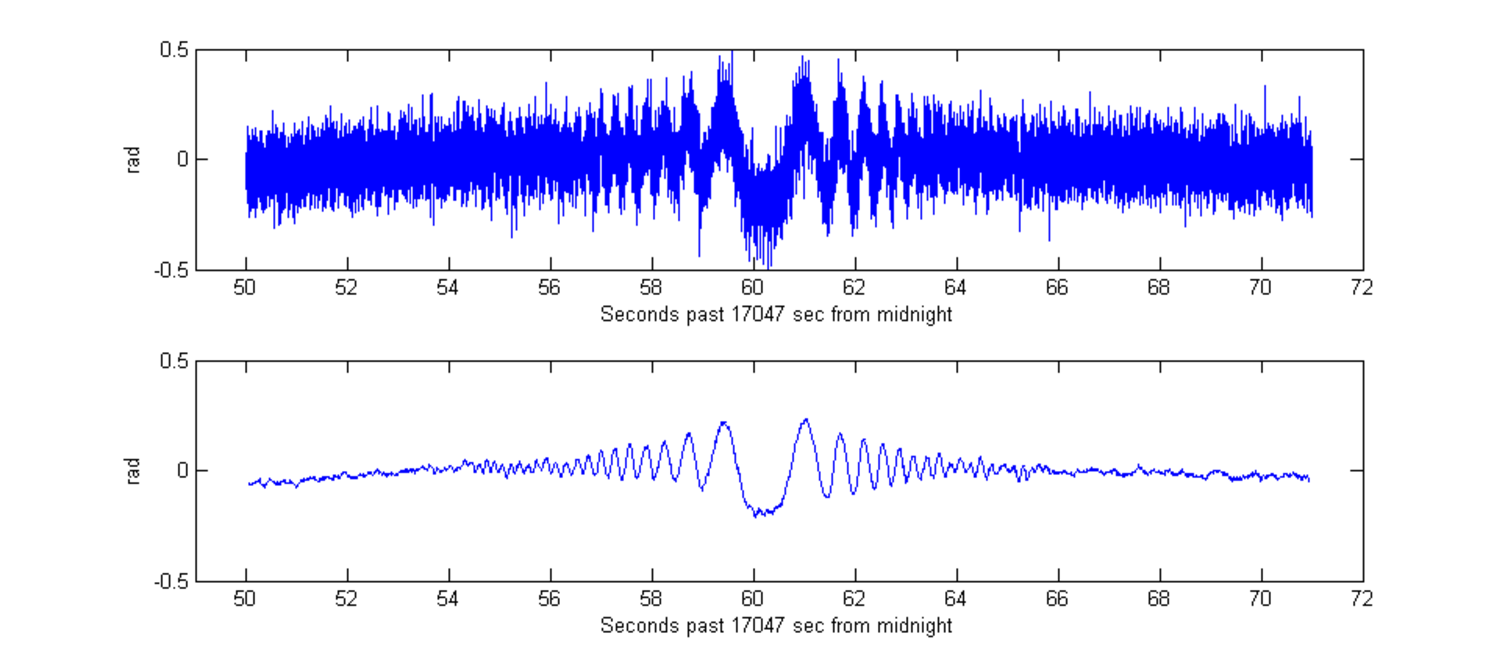
\includegraphics[page=1,trim={2cm 0 2cm 0},clip,width=6in]{RingletPhase2009.pdf}
    \caption{Attachment from Paulo Tortora}
\end{figure}
\begin{figure}[H]
    \centering
    \captionsetup{type=figure}
    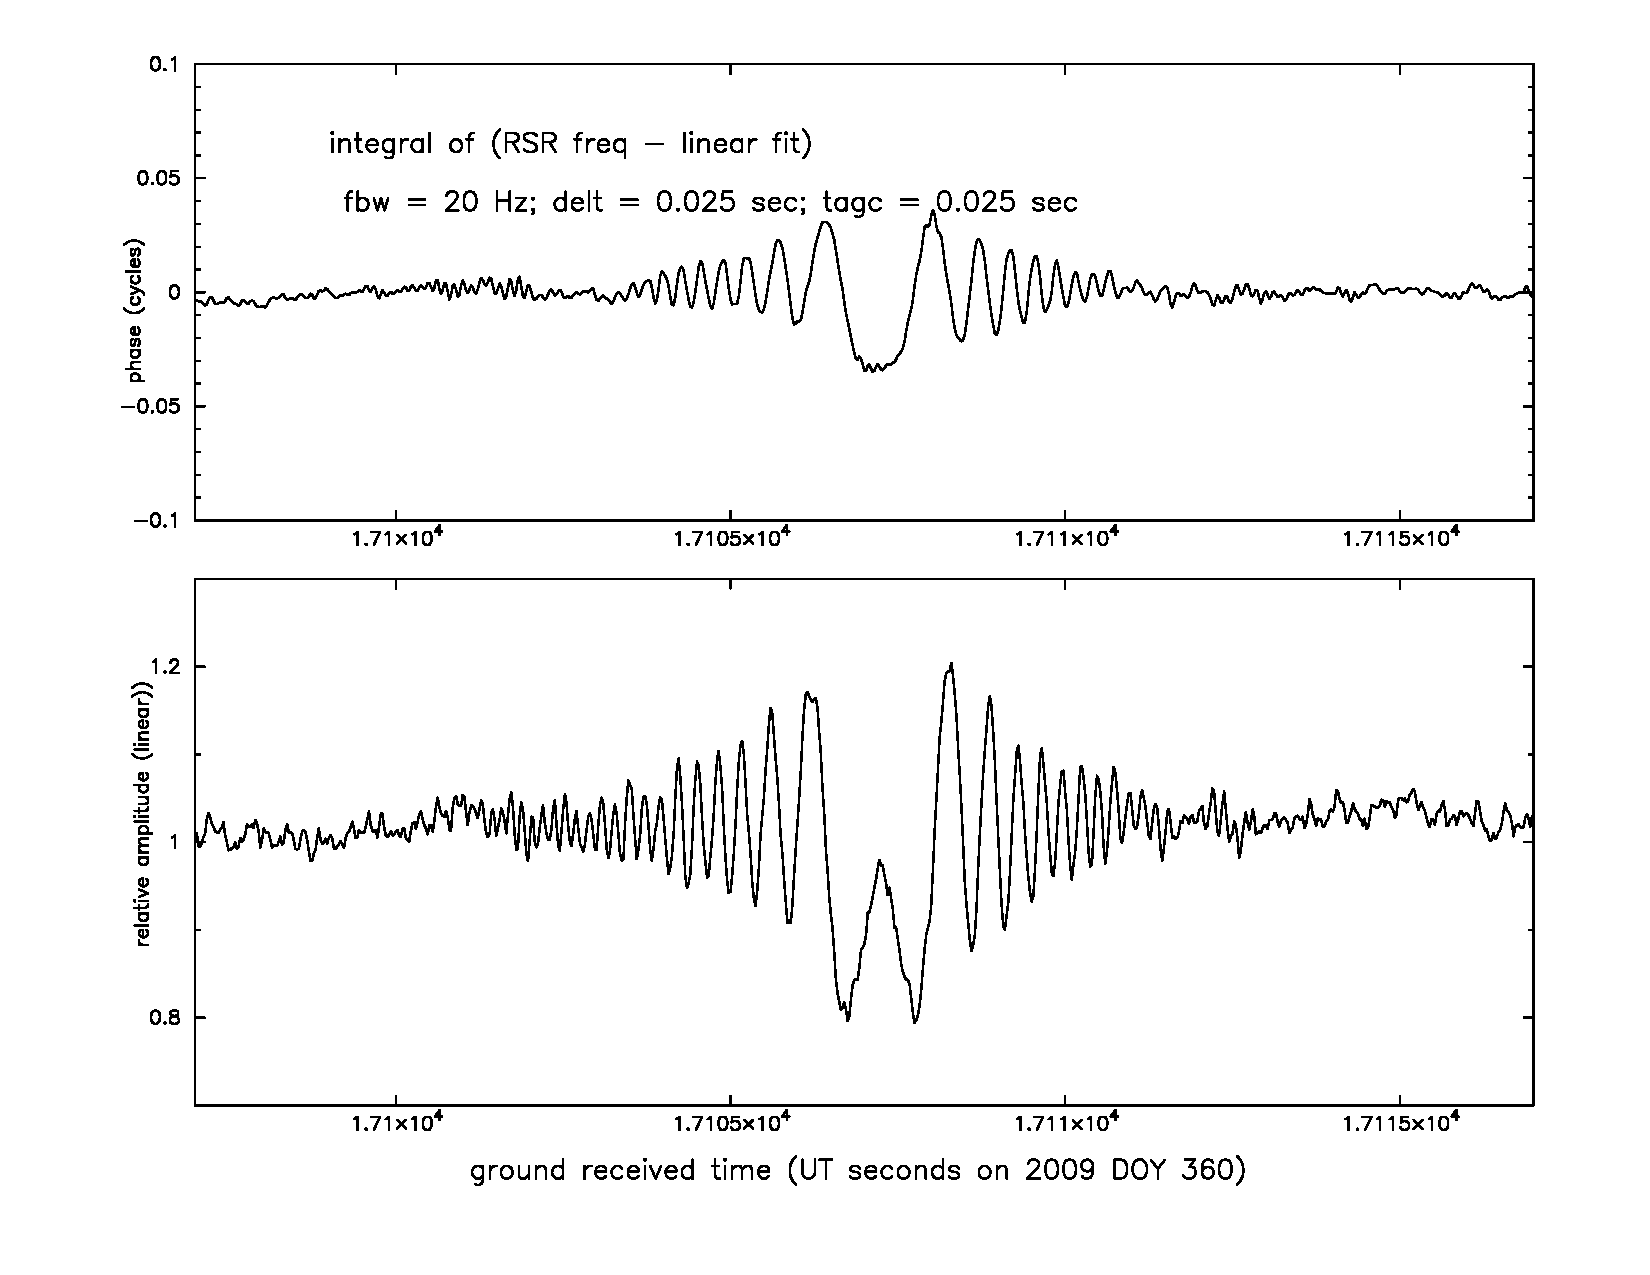
\includegraphics[page=1,trim={2cm 0 2cm 0},clip,width=0.49\textwidth]{plot_amp_phase_jwa.pdf}
    \hfill
    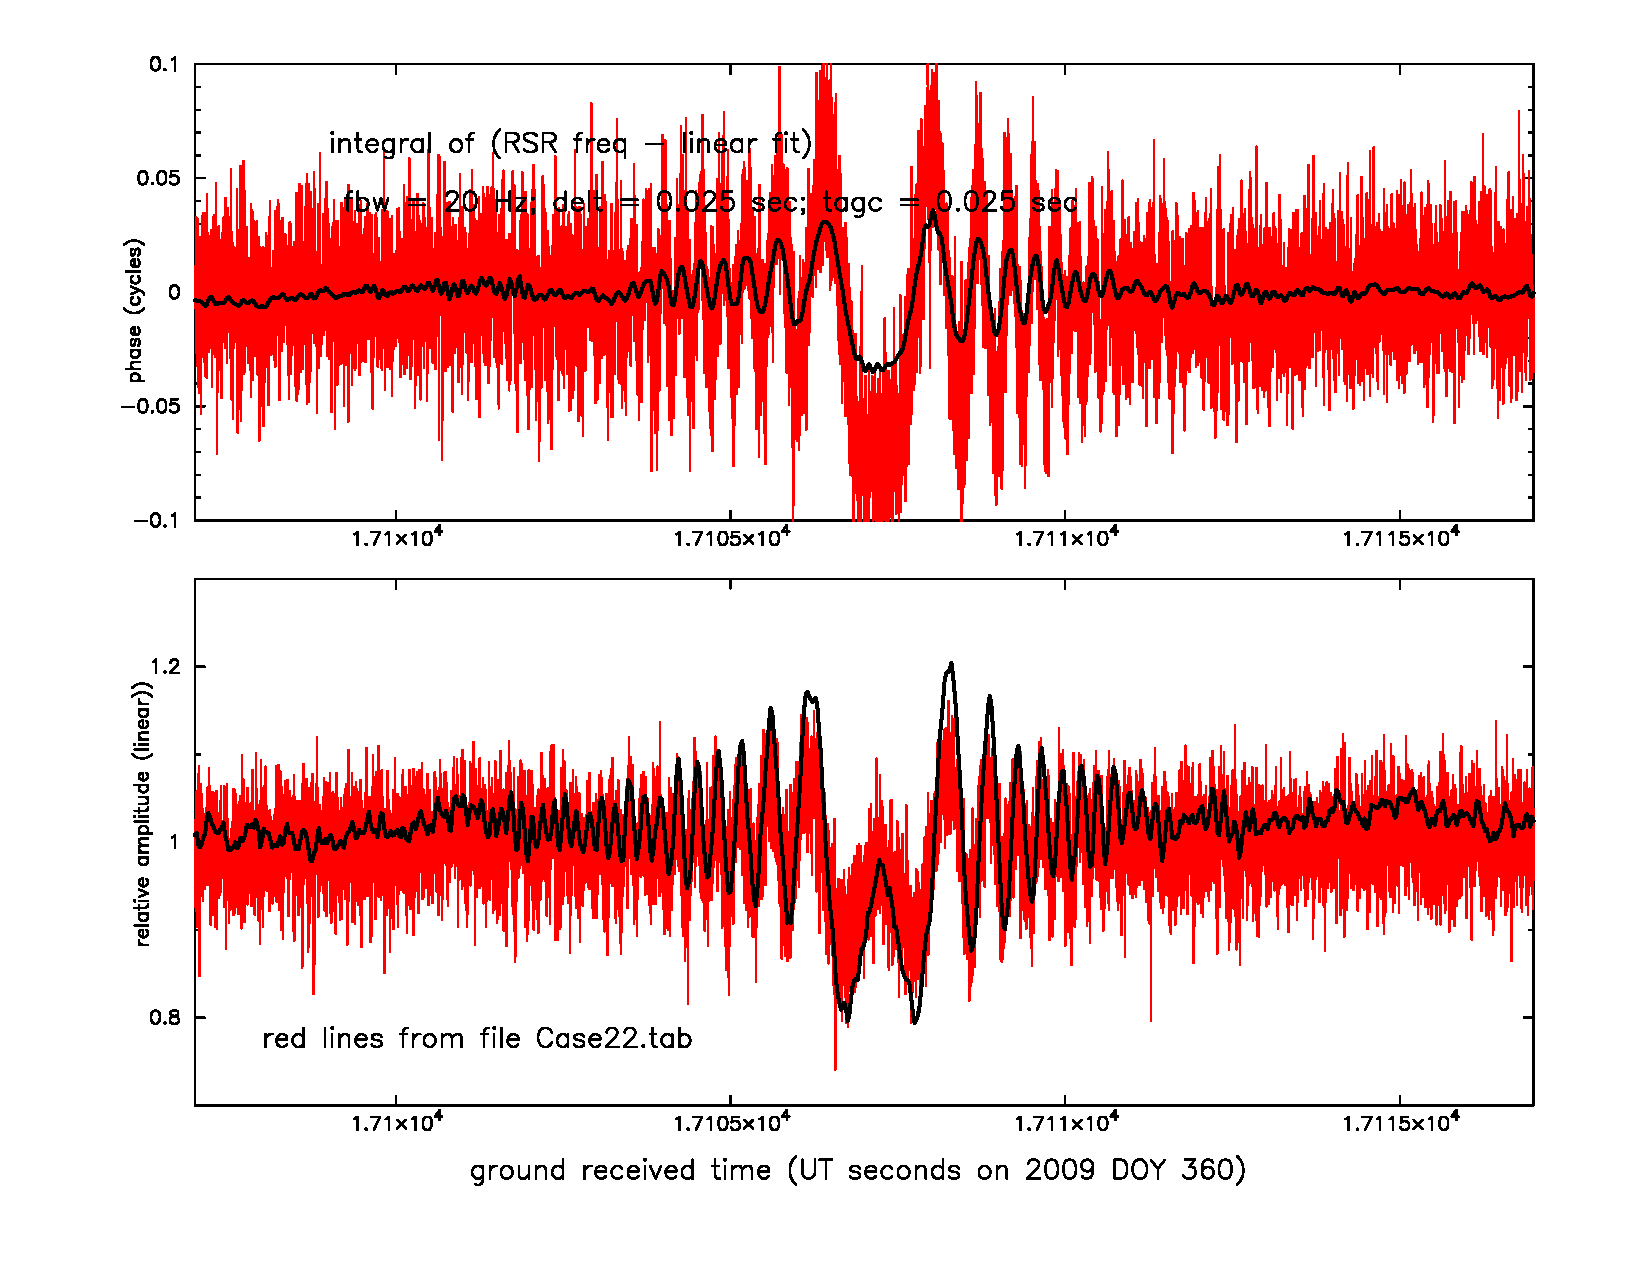
\includegraphics[page=1,trim={2cm 0 1.5cm 0},clip,width=0.49\textwidth]{plot_amp_phase_compare.pdf}
    \caption{Attachments from John Armstrong}
\end{figure}
I'd like to compare our team's approaches to estimating power and phase from RSS RSR recordings of ring occultations, so that we can optimize the retrieval of high-resolution diffraction-corrected ring profiles. To that end, I've provided examples for observations of the F ring - a narrow ringlet isolated in free space. Given the complex signal (power and phase), the diffraction-corrected radial profile can be obtained by performing a Fresnel transform, but the quality of the retrieved profile depends strongly on the quality of the received signal as extracted from the RSR. I'd be very grateful if you would use your own algorithms to extract power and phase, and compare them to the results I've obtained. I estimate the power from the sum of the signal in the vicinity of the maximum signal in the power spectrum. This can probably be improved by performing a fit to the peak power rather than just adding adjacent samples, but I have not explored this part of things yet. I'm more concerned about extracting the phase. In this example, I've determined the phase simply by taking atan(<Q>,<I>), where <I> and <Q> are the time-averaged I and Q values directly from the RSR, and the final phase is computed by unwrapping the phase and removing the local drift. That is, I do NOT use any frequency information directly, and I suspect that the phase retrieval can be made more robust and require less fiddling if I use another approach. This folder contains the results of attempts to retrieve the power and phase of the RSS X-band signal in the vicinity of the F ring from the Rev 123E X63 observations. 16 KHz data on the PDS Atmosphere node can be found \href{https://pds-atmospheres.nmsu.edu/cgi-bin/getdir.pl?volume=cors_0302&dir=SROC10_359/RSR}{here}, S56SROE2009360\_0145NNNX63RD.2A2
1 KHz is on the SOPC: /data/RS\_Share/s56-rev123-rsr-data/S56SROE2009360\_0145NNNX63RD.2A1
I've centered on the data interval 50 to 70 sec after 17047 sec past midnight on the day of the event. Contents of this folder:
\begin{itemize}
    \item README.txt - this file
    \item rsr\_info\_v3a\_20170518a.pdf - plot of Dick's retrieval, averaged to 0.02 sec res
    \item rsr\_info\_v3a\_20170518a.pdf - plot of Dick's retrieval, averaged to 0.02 sec res
    \item Case22.tab - table of Dick's retrieved power and phase, at 0.002 sec resolution.John Armstrong provided some estimates of power and phase as follows:
    \begin{itemize}
        \item I had a first look at the 1kHz RSR file and got the attached. The PLL parameters I used were at the limit of what my code allows (w/o some modification; actually:  a little beyond the limit, in that I allowed
        some aliasing of the freq(t) to try to get better time resolution).  I
        used a linear fit to the f(t) data at the nominal time +/- 2 minutes (shown in the attached) and then integrated the difference between the estimated RSR freq and the linear fit. More interesting is that, at the resolution my code allows, I see pretty significant freq variation from point to point — suggestive that I am *not* resolving the real variation in my analysis.
    \end{itemize}
    \item ringlet\_closeup.pdf - John Armstrong's retrieval using the 1 KHz file ringlet\_2min.pdf - John Armstrong's regional retrieval using the 1 KHz file.
\end{itemize}
When you have a chance, would you compare your results with my tabulated and plotted results, and describe the technique you used to estimate both power and phase? -Richard French
\par\hfill\par
Hi Dick, I did my homework during the PSG and generated the attached plot. The only difference is that the top panel is raw data at 1KHz, the bottom panel is compressed at 10Hz (0.1s). I think they seem pretty similar to yours, I don’t expect any processing to do better than what you got already. Is this what you were expecting from us? -Paolo Tortora
\par\hfill\par
Hi Dick, I attach three things:  a plot of my estimated amplitude and phase, a plot with my estimates superimposed on the ones you sent in file “Case22.tab”, and a list of the points in my plot (SPM, amplitude (linear), and phase (cycles)).  The original data file was S56SROE2009360\_0145NNNX63RD.2A1 (X-band; DSS63; 1kHz). I ran my PLL (with, for my reference: fbw = 20; delt = 0.025, tagc = 0.025). I did a linear fit to the frequency +/- 1 minute from the ring and subtracted the fit, then integrated the result to get phase.  I subsequently smoothed the estimated amplitude and phase.  The smoothing is slightly different in each case because the PLL parameters can’t be adjusted to give exactly the same Fourier content at each output (due to the historical way the program was written, since I did not care about amplitude except to stabilize the input to the phase detector).   The intent was to get approximately the same Fourier content in the phase and amplitude in the final file. The output is at 0.025 second intervals in the attached file. My disclaimer is:  The procedures that Essam and you use are clearly far superior to what I did here.  I am using my code in a way that was not intended in the design and am concerned (in particular, relevant for your application) that the group delay in the processing for the phase and amplitude estimates may not (quite) be the same.  I offer the attached if this level of processing might be useful for the comparison you mentioned in your original e-mail. -John Armstrong
\subsubsection{\footnotesize RE: Question About Time Tags for RSR Files}
In the process of developing a software pipeline for RSS ring data, a question has arisen about the exact meaning of time tags for RSR files. For simplicity, consider a 1 kHz file, starting at $1000$ SPM (seconds past minute) with $\Delta t$ between samples being $0.001$ sec. Three questions:
\begin{itemize}
    \item Does each sample     represent an average over $0.001$ sec, or some kind of instantaneous measurement?
    \item In the either case, should the time tag for the first bin be CENTERED  on the first bin - that is, between $1000.0000$ and $1000.0010$ (and thus be $1000.0005$)? or should it be $10000.0000$, or even $999.9995$ (in which case it would represent the average of the previous $0.001$ sec and be written out at $1000.0000$)?
    \item What do you gravity folks assume, Paolo and Luciano?
\end{itemize}
As a practical matter, this is not important, since the spacecraft location is not known to this level of precision, but when we document our code in detail, I'd like to know what the official answer is, and not just dismiss it as unimportant. -Richard French\par
The time tags are given by that RSR at the beginning of every second. What follows is all the samples at whatever sample rate. So the first time tag in your example should be $1000.000$, and this sample represents the first millisecond from $1000.000$ to $1000.001$. In order to make your own computations and time tag in the middle of an interval, you need to add half that interval, in this case $0.0005$. For example, one thousand milliseconds tagged by the RSR from 1000.000 to 1000.999: 1000.000, 1000.001,..., 1000.998, 1000.999, each covers one millisecond centered at 0.0005: 1000.0005, 1000.0015,..., 1000.9985, 1000.9995. The average works out to $1000.5$, which covers the second which began at $1000.000$. The time tag for the first second of data is placed at $1000.5$. -Danny Kahan
\subsubsection{\footnotesize RE: Padding - RSR to Power/Frequency}
Thanks again, Paul, for all your help with this. I've been reading through your codes and doing a bit of reading about signal processing as well, so I am now in a position to ask some sensible questions. As a starting point, it would be helpful to go over with you - by phone or email:
\begin{enumerate}
    \item your recommended standard settings for the port.input file for 16kHz RSR data
    \begin{itemize}
        \item Depends on how big your data chunk is. If you’re using
              64 x 512, then the frequency sampling is $\sim$ 1/4 Hz,
              which is good enough.  If it’s only 8, then it’s 2 Hz,
              which is too much. I’m currently running the S07 file
              you’re using, and I ran portspctrm with 8 1 1 with a
              pad of 20, so my port. input is:
            \begin{itemize}
                \item 0.86400. 1.22344945e+03 0. 0.0e0 1 20 1 1 0 0 5. RSR X.
            \end{itemize}
        20 is probably too much padding, though, so it’s taking a long time. -Paul Schinder
    \end{itemize}
    \item Poca steering for the case of rsr data - do you use a
          steering file?
    \begin{itemize}
        \item Generally I've steered using two different methods for
              two different reasons.  Back in the Galileo days when
              all we could do was the ionosphere because of the low
              power, we'd steer using ``Doppler steering'', simply
              by using a prediction of the frequency that should be
              received if the ray path is entirely in vacuum using
              the measured USO frequency, something like LMBTRK tries
              to do.  But the steering that was used on the
              s10sroe2005123\_0740nnnx43rd.2a2 file seems to have
              been a little off, so that it's about -13 Hz in vacuum.
              Steering to Doppler will remove that offset, so that
              it’s 0 Hz in vacuum as intended.  The steering is done
              by adding a phase to the original data points, while
              recomputing the steering polynomials to reflect the
              adjustment.  In principle you could put them both
              together into a new RSR file, but I don’t do that.
              [The second method we’ve tried was a few years ago
              when one of the referees of our first Titan paper
              asked about diffraction at the surface.  The only
              way to backpropagate that was to steer to the atmosphere
              as we found it, so we just steered so that the original
              PSgalfreq.out we found from the data was zero Hz
              (steering the atmosphere out), and then backpropagated
              around that.] So after I steer my port.
              input will probably look like:
            \begin{itemize}
                \item 32000. 34000. 1.22344945e+03 0. 0.0e0
                      1 5 1 1 1 1 5. RSR X
            \end{itemize}
            and I’ll start saving individual spectra to look at and
            to visualize as a group.  We used to do that a lot for
            Galileo, and I did it again a few years ago when looking
            at Titan.  I think Essam has shown plots like this for
            ring data as well. -Paul Schinder
    \end{itemize}
    \item The meaning of beta.
    \begin{itemize}
        \item Beta was an attempt to predict where the signal was going.  We knew that when we dropped below the ionosphere and reached the top of Jupiter’s neutral atmosphere the frequency would take a sudden change in direction, but because we also lost the signal from the low gain antenna at that point we couldn’t see where the signal was going.  So we guessed, and hoped that we could eke out a bit more signal from the data.  It never really worked (we could fool ourselves a little, but not that much), and beta is no longer used. -Paul Schinder
    \end{itemize}
    \item How your continuous Fourier transform works?
    \begin{itemize}
        \item It’s a discrete FT: $\mathcal{F}(f) = \sum V_n e^{2\pi i n f t_n}$. Do the FFT, find the FFT frequency with the maximum power, go a little below and above that frequency (as you can see above, +/- 5 Hz), crawl along $\mathcal{F}(f)$ until you find the peak power $\norm{\mathcal{F}}$. -Paul Schinder
    \end{itemize}
    \item The consequences of using different window functions.
    \begin{itemize}
        \item As I remember when I played around with it long ago, using any window helps, not using one may produce artifacts.  But I don’t remember the details.  What I learned about windows I got from Numerical Recipes, and there’s a good discussion there. -Paul Schinder
    \end{itemize}
    \item whether you ever try to fit a model function to the fft peak in order to refine the frequency
    \begin{itemize}
        \item Yes, and some of that is still in the code, although maybe not in a working state.  When we started using a discrete FT, we stopped trying to do that, since it serves the same purpose. -Paul Schinder
    \end{itemize}
\end{enumerate}
I'm going to create a data.out and poca.out file for a small snippet of the Rev 007E X43 RSR file that corresponds to the ringlet that Essam used as an example in his Data User's Guide, to see how the power vs time and phase vs time compare, using a variety of input parameters. Once I understand your code better, I think I may try to write a special-purpose version of it for ring data as a pre-processor before I tackle diffraction corrections - but before doing that, I need to understand  some of the above issues. If some of them require detailed discussion we can do that by phone. -Richard French
\begin{figure}[H]
    \centering
    \captionsetup{type=figure}
    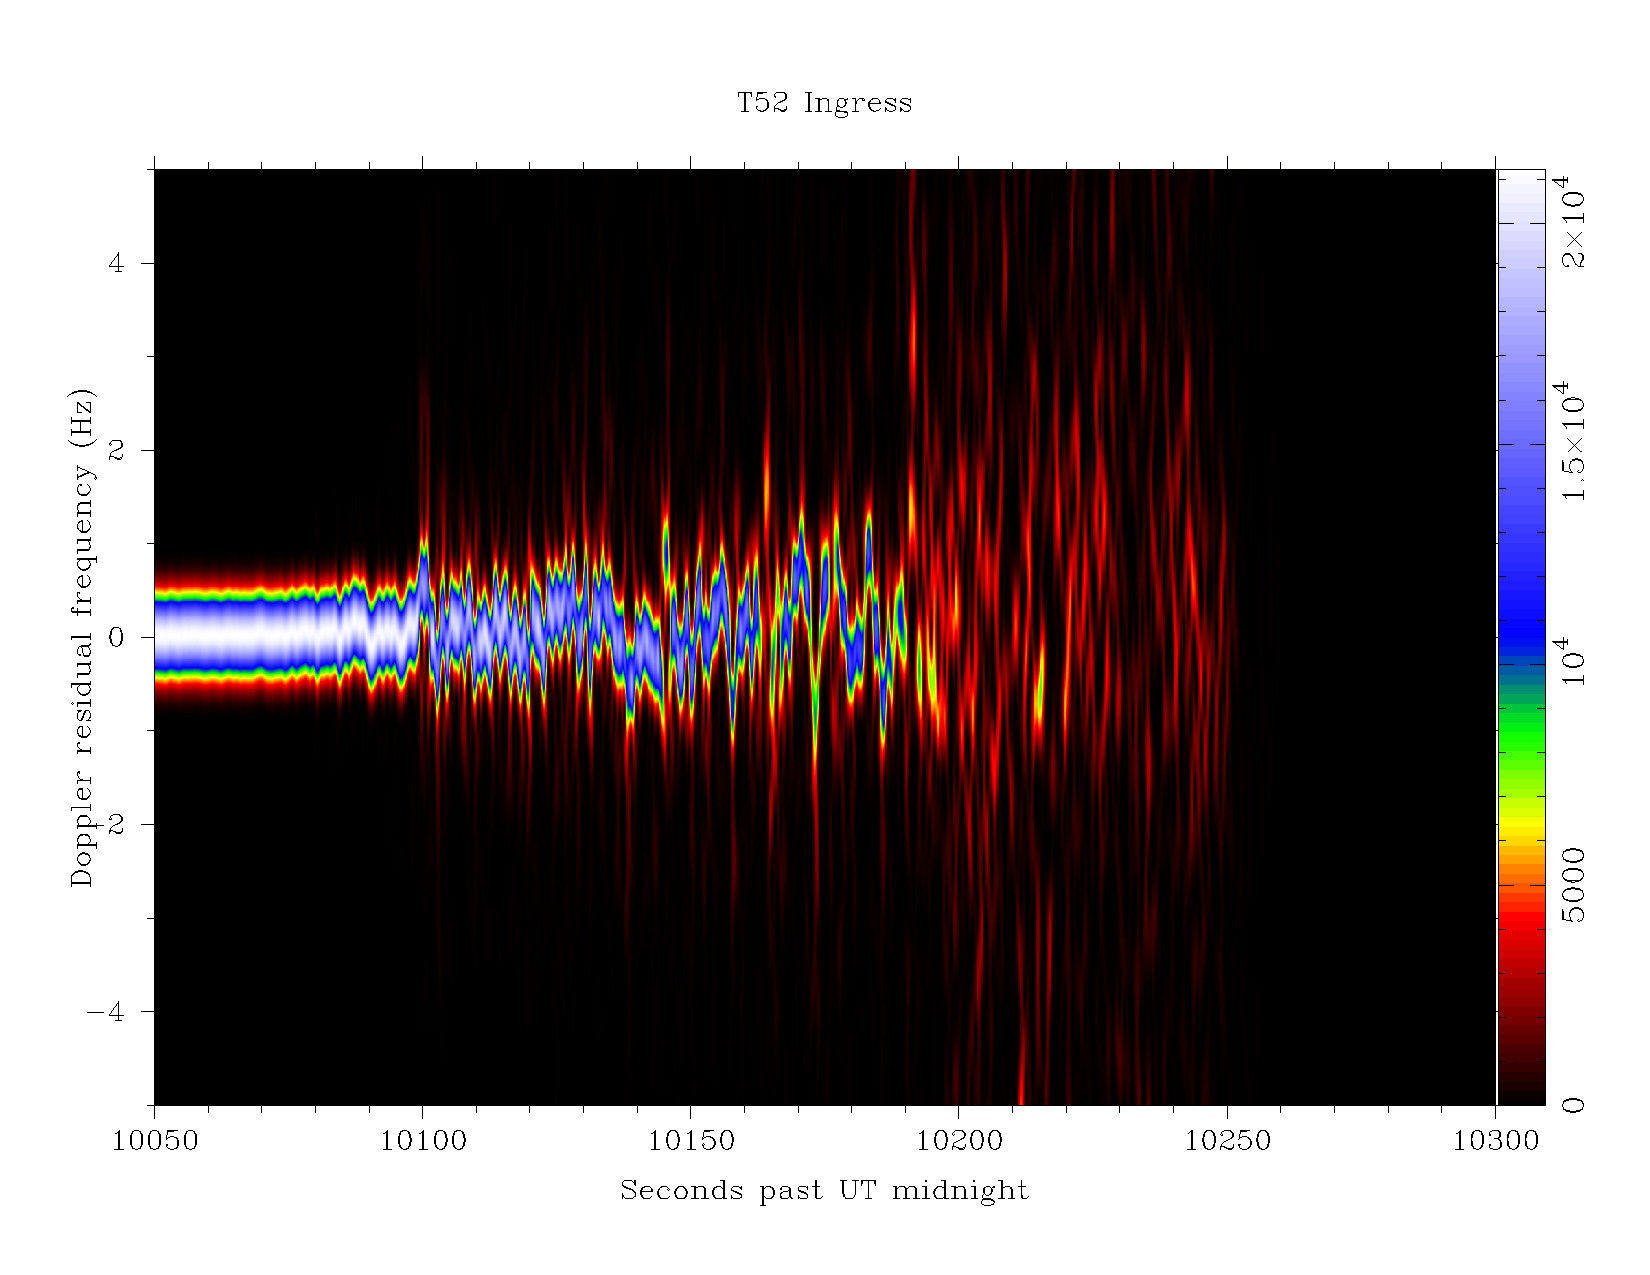
\includegraphics[page=1,width=3in]{non_copy.pdf}
    \hfill
    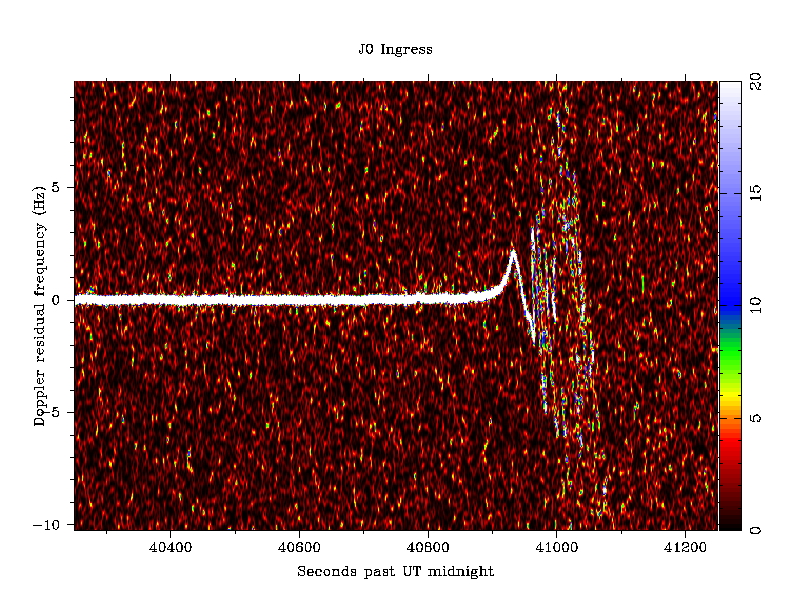
\includegraphics[width=3in]{non.png}
    \caption{Attachment from Paul Schinder}
\end{figure}
\subsubsection{\footnotesize RE: 1 KHz vs 16 KHz files}
We're trying to finalize our data pipeline for ring analysis, and I still have some questions about the best way to extract power and phase at high time resolution (say, at 100 Hz). 
\begin{enumerate}
    \item I had the naive idea that we ought to be able to get identical results when we analyze the 1 kHz files and the 16 kHz files, but I'm finding that the noise floor I derive for the 16 kHz files is larger than for the 1kHz files, which I'm not sure I understand. 
    \begin{itemize}
        \item Yes, you do get more noise because you’re using a wider bandwidth.  You’re not cutting off the noise above 500 Hz or below -500 Hz the way you do with 1 kHz.  You’ll see the same thing if you analyze 50 kHz or 100 kHz files. -Paul Schinder
    \end{itemize}
    \item Given a 1kHz and 16 kHz file from the same DSN for the same event, would you expect to get very similar/identical results from portspctrm for the two data files? If so, what changes to the input parameters would you need to make to ensure that equivalence (targeted to trying to get high time resolution for the derived power and phase).
    \begin{itemize}
        \item Yes, they should be very similar, but I don’t think you can ever guarantee they’re identical.  I just checked some files from S169 I have lying around and they’re within  mHz of each other when the signal is strong, but not identical. -Paul Schinder
    \end{itemize}
    \item For example, I analyzed the end of mission files with the command line parameters 1 1 1 (use 512 points per frequency point, skip 512 points per timestep) which at 1kHz gives a time resolution of 0.512 s.  If  we’d had 16 kHz and needed a better estimate of LOS, I probably would have used 8 1 1 (use 8*512 points, skip 512) which at 16 kHz is 0.512/16 s resolution, but with the caveat that there might be some unwanted correlations or smearing of the power drop off right at the end because of the chunking together of 8 * 512.  I’d probably pad that to get the frequency resolution up, too.
    \begin{itemize}
        \item Another question is this - does padding affect primarily the frequency resolution of your derived result (my supposition), or does it also affect the power estimation? -Paul Schinder
    \end{itemize}
\end{enumerate}
The intent is simply to increase the frequency resolution.  Since you’re adding zero power, it shouldn’t affect the power.  I’ll have to double check to make sure, though. -Richard French\par
Thanks, Paul - we'll play around with this and see if we can make sense of it all. We are at the point now where we can get close to the same results that Essam gets for our estimates of power and phase, but we are not using any FFTs to do so - we are simply averaging the 1 kHz I and Q values and then taking $I^{2} + Q^{2}$ of the 0.25 km resolution sums for the power, and effectively atan(Q,I) for the phase, which we then adjust by removing the drift in frequency due to the imperfection of the predicts calculation. The problem with this approach is that the raw I and Q have noise in them that, for longer integration times, can be filtered out using FFT's by isolating the power peak in the FFTs, and getting a good frequency estimate from padding the FFT. Then the phase can in principle be recovered by integrating over $\delta freq\cdot dt$. What I'm trying to sort out is whether we can do better by using FFTs with the 16 kHz files to compute the power and frequency/phase at, say, 0.25 km resolution, than the method we are using now: just take the 1 kHz raw I and Q, compute $I^{2} + Q^{2}$ for power, atan(Q,I) for phase, and then correct for the phase drift with time of the predicts error. Our results in hand are not too bad, so if necessary we can proceed with our straightforward approach, but it relies on using the 1 kHz files at the moment, which are not part of the PDS archive. Ideally, we would use the 16 kHz files, even if computationally slower, so that we don't have to archive the 1 kHz RSR files, too. -Richard French
\subsubsection{RE: SNR Ideas for the Record}
\begin{enumerate}
    \item Write to Dick Simpson and Dave Hinson and ask them to compute thermal noise level for Rev007E 1 kHz file
    \item I think threshold optical depth is too optimistic - it accounts only for thermal noise, which applies only for the most opaque parts of the ring - and in any event our post-inversion profiles show a more realistic estimate of what the thermal noise actually is.
    \item For tenuous parts of the ring, such as the C ring, we care more about the minimum optical depth variation that we can believe in the data. For this, I think we can simply take the stdev of the normalized free-space signal (after inversion) at the actual spacing of the inverted profile (ex: 0.25 km for 1 km resolution data) and convert that to optical depth. That is a practical limit to the MINIMUM reliable optical depth variation. 
    \item Using this value, plot tau for the the tenuous regions of the C ring and Cassini Division on a scale where this minimum optical depth is plotted as a horizontal dashed line - it should pass through the excursions of the free-space signal.
    \item Another approach to estimating the limit of useful resolution is to determine the rms of the phase, in cycles, after removing the frequency offset, and finding the optical depth at which this rms phase exceeds 0.1 cycles. This should be a function of spatial resolution. Glenn can calculate this from the frequency-offset-corrected phase prior to inversion. An easy way to identify the limiting optical depth would be:
    \begin{itemize}
        \item plot rms of phase vs radius - there will be areas of opaque rings where this gets big and saturates.
        \item be aware that there will be blips where the rms phase will be artificially big because of phase wrapping, so plot as points instead of as lines, perhaps.
        \item plot tau vs radius on a separate panel
        \item plot rms of phase vs tau - there should be a trend of increasing rms with tau
        \item When rms of phase exceeds 0.1 cycle, this is a practical limit to the reliability of the phase evaluation and thus to the details of the ring structure at this resolution.
    \end{itemize}
\end{enumerate}
\subsubsection{\footnotesize RE: phase wrapping - one more suggestion - and a math problem for Ryan}
Another quick idea to help solidify our understanding of the origin/solution of the phase wrapping problem. You might try running some intermediate cases of the number of points in the FFT: 2048, 4096, and 8192 come to mind as obvious possibilities. I expect that you'd see a trend in the magnitude of the difference in the phase shifts with the degree of averaging. I'm struck by the large DC phase shift, in addition to the slope that you demonstrate in the middle panel of plots - I would expect that this would increase rapidly with the amount of averaging, and it would be interesting to plot just that DC offset as a function of the number of points in the FFT divided by 1024, your base case. It might have some interesting curvature, and this is something that you could relate to the magnitude of the error in Simpson's rule, which is the method you are using for integration. Ryan would probably have some interest in predicting the error in Simpson's rule as you increase the step size, and seeing if your results agree. Similarly, if my hunch about the origin of the problem is right, you should find improvement as you successively increase the number of sub-points in your spline interpolation of the 16384 case from 2 to 16 (or perhaps even more). If all of this works, I think we will have a more robust solution of the frequency offset problem, but we'll just have to see! -Richard French
\subsubsection{\footnotesize RE: How to Read Geometry Files in IDL}
\begin{lstlisting}[language=IDL]
tc_geo = rdcol(geofile_tc, 1, 99999999, [1:18])
t_OET_spm_tc            = tc_geo[0,*]
t_RET_spm_tc            = tc_geo[1,*]
t_SET_spm_tc            = tc_geo[2,*]
rho0_km_tc              = tc_geo[3,*]
phi_RL_deg_tc           = tc_geo[4,*]
phi_ORA_deg_tc          = tc_geo[5,*]
B_deg_tc                = tc_geo[6,*]
D_km_tc                 = tc_geo[7,*]
rho0_dot_kms_tc         = tc_geo[8,*]
phi_RL_dot_kms_tc       = tc_geo[9,*]
F_km_tc                 = tc_geo[10,*]
R_imp_km_tc             = tc_geo[11,*]
R_sc_x_km_tc            = tc_geo[12,*]
R_sc_y_km_tc            = tc_geo[13,*]
R_sc_z_km_tc            = tc_geo[14,*]
R_sc_dot_x_kms_tc       = tc_geo[15,*]
R_sc_dot_y_kms_tc       = tc_geo[16,*]
R_sc_dot_z_kms_tc       = tc_geo[17,*]
\end{lstlisting}
\subsubsection{\footnotesize RE: Phase Calculation to Try}
I don't think we've yet tried an idea I had for computing the phase that might be more accurate than what we are doing now. Instead of using $phase = atan(\langle Q \rangle,\langle I \rangle)$, where the $\langle \rangle$ represents an average of measurements straight from the RSR (which I think is what we are doing now), the idea is that we use an analogous method to what we are doing when we compute power. 
\begin{enumerate}
    \item Take the power spectrum of a small chunk of data - 16 points, I think, for 1KHz files.
    \item Find the location of the peak power and its adjacent m neighbors and add them up - that, I think is how we compute power now.
    \item Let those indices in the power spectrum that contribute to the power be an array L.
    \item Set all of the other elements in a copy of the FFT that produced the power spectrum to zero.
    \item Take the inverse FFT to reconstruct a time history of the reconstructed $I_r$ and $Q_r$ over those 16 points.
    \item Compute $\langle I_r\rangle^2 + \langle Q_r\rangle^2$ and compare it to the power you computed from the power spectrum itself - these should agree, perhaps to within a constant normalization factor.
    \item Compute $phase_{r} = atan(\langle Q_r\rangle ,\langle I_r \rangle)$ and compare to phase as computed above. 
    \item Try this for a variety of m neighbors.
\end{enumerate}
Ideally, this would give good agreement where the signal is strong, but give improved results where the signal is weaker, as in the center of an opaque ring. Would you make a plot of the results for the Maxwell Ringlet and Huygens Ringlet, to see if this works at all? (For starters, you can do this just for the I and Q without having to apply the frequency offset part, unless it's just as easy to do the entire process to compute the final phase.) Compare the results to our previous method for both phase and power, and to Essam's from the savefile that gives the pre-Fresnel-inversion phase and power. Then make a final set of plots to compare the methods and make a decision about which method is best for computing the phase. If so, then let's use this method to compute the phase for the full. Rev007E to confirm that it works.
\subsubsection{\footnotesize RE: Calculating the Noise Power}
MTR86 claims that the RSR data have Gaussian, uncorrelated thermal noise - a reasonable assumption - but it remains to be seen that the actual noise in the data is dominated by thermal noise, and the time periods over which this is a valid approximation. MTR86 compute the normalized noise power as:
\begin{equation}
\langle P \rangle_{\textrm{MTR86}} = \frac{\sigma^2(\langle I \rangle) + \sigma^2(\langle Q\rangle )}{(\langle I \rangle^2 + \langle Q \rangle^2)}
\end{equation}
where $\langle \rangle$ represents a time average of the data. I would instead compute the normalized noise as
\begin{equation*}
\frac{\sigma(\langle P \rangle)}{\langle P \rangle}
\end{equation*}
Where $\langle P \rangle = \langle I^2 + Q^2 \rangle$ .The difference is that Essam takes averages of I's and Q's before squaring, whereas I compute the power for EACH data point, and then average those to get the power. I think these would give the same answer if I and Q had only thermal noise added and successive data points were uncorrelated, but the RAW RSR data don't satisfy this assumption, because there is a frequency drift of about 10-12 Hz that should be visible as a sine wave in I and Q, which would result in an overestimate the actual thermal noise using Essam's expression because most of the variation in I and Q would be due to the frequency drift. It may be that implicitly Essam assumes that the frequency drift has been removed prior to using his equation. A related issue that we should test is whether the noise power scales with the integration time in the fashion that Essam predicts. Here is a set of tasks to help sort this out: (do these for BOTH the 1 kHz and 16 kHz files)
\begin{enumerate}
    \item Select a range of data in time corresponding to a range of ring plane radius prior to or after the main rings, where the signal level is smooth and not affected by the atmospheric occultation or is especially noisy due to low elevation angle. Choose about 2 minutes of data, for starters.
    \item Use the equations above to compare and plot $\langle P\rangle_{\textrm{MTR86}}$ and $\langle P \rangle$ as a function of the averaging time for both the raw I and Q values, and separately for the frequency-offset-corrected I and Q, but still at high time resolution, where for the 1 kHz file you should let the averaging times vary between 0.01 to 10 seconds (they don't need to be equally-spaced intervals across this span). $\langle P \rangle$ should be expressed in dB (or you can just plot $\langle P \rangle$ on a log-y axis).
    \item Plot I and Q from the raw RSR data over a few-second interval from both 1 kHz and 16 kHz files, for a variety of nsum values, increased until (I hope) you can see a sinusoidal signature in the raw I and Q, uncorrected for the frequency drift.
    \item Interpret the results - compare the results of the two equations - are there domains when both are in agreement? Over what time intervals? Does the trend of <P> with averaging time match Essam's equation? is SNR0 (1/<P>) for 1-second time averages about 53 dB, as Essam found for Voyager?
\end{enumerate}
\subsubsection{\footnotesize RE: Rev7E kernels from easy data that were used for figures in interim report}
\begin{lstlisting}[language=bash,basicstyle=\footnotesize]
SPICE_FILE_NAME = {"050606R_SCPSE_05114_05132.bsp", "cpck26Feb2009.tpc",
                   "naif0009.tls", "earthstns_itrf93_050714.bsp",
                   "earth_000101_090604_090313.bpc"}
\end{lstlisting}
\subsubsection{\footnotesize RE: Organization of RSS Ring Profiles}
Hi, Mitch - We're preparing a sample submission to the PDS of reduced Cassini RSS ring profile results, as an example of the data we plan to submit for the entire set of RSS ring occultations, if we can do this with our current level of effort. There are some high-level decisions PDS needs to make about how to organize the data and how to interleave them with (or isolate them from) Essam's contributions. As you know, we won't have my preferred solution of a single set of submissions using the equivalent of Essam's code, since he does not want to share his algorithms or code with me, so we are going our own way in developing a best-effort open-source software data pipeline that will do the best we can (and, we think, may be very close to Essam's but not bit for bit the same, and without his vetting) - we'd like to archive representative results from this open-source pipeline, including results at higher resolution than the 1 km profiles Essam has promised to provide. (He's also indicated that he might archive higher-resolution products, but only after he has published the results, and he has not identified either a target date for that task, or the specific results he'd plan to include.) In this situation, I think it might make sense for our PDS archive to be separate from Essam's, rather than intermingled. We would provide some high-level summary at the top to users that says:
\begin{enumerate}
    \item This set of profiles was produced by the RSS team using team member software (Essam's contributions).
    \item This other set of profiles (probably more complete and certainly at higher spatial resolution) was produced by thoroughly documented open-source software that enables any user to reproduce the final profiles, beginning with the raw RSS data.
\end{enumerate}
Once we have some of Essam's high-resolution profiles, we'll be able to compare how the two sets agree. I fervently wish that we had a single set of data to submit, but I am firmly committed to producing open-source software, and I don't think it makes sense to archive the software without also archiving the results that come out of using the software. Would you and Mark give some thought to your preferred way of ingesting these two different sets of ring profiles (Essam's and mine), both in terms of organization and target audience? Our proposed directory structure is similar to the existing one, but we intend to include additional columns in many of the existing data files, and to add a new data file type that contains the normalized diffraction pattern (power and phase) that goes into the Fresnel inversion routine. Finally, we will also provide a comprehensive data catalog, images of occultation geometry as viewed from the earth, elevation plots that show which data files are best for each individual occultation, etc. - these will need a home in our data archive as well. Thanks, Mitch - no immediate rush, but I would like to chat with you about this once you've had a chance to digest this message and consult with Mark. -Dick\\
Hi Dick, I just wanted to let you know I did get your email. Mark and I have been completely out of synch this week. We’ve identified an intersecting gap in our schedules Thursday afternoon when he and I can discuss our responses. I should be ready to chat with you on this Friday if you have some time. I should be available from about 9:00am until sometime early afternoon. -Mitch
\subsubsection{\footnotesize RE: Radial Locations of Waves and Features for Revs 125-133}
Would you write a short IDL procedure to enable you to make plots of the following regions, so that you can easily tweak the plot scales and reproduce the plots without difficulty? Use the recent low-inclination reconstructions and perhaps overplot different retrievals in different colors so that we can see by eye which is best. In the c ring: +/- 50 km relative to the radii shown here, then zoom in to see the structure of the waves:
\begin{itemize}
    \item Mi 4:1 m=2  74890 km  1.1$\pm$0.5 g/$\textrm{cm}^2$  0.16$\pm$0.09  0.18$\pm$0.13 g/$\textrm{cm}^2$
    \item W74.66 m=-7 74666 km  0.7$\pm$0.2 g/$\textrm{cm}^2$  0.09$\pm$0.03  0.15$\pm$0.09 g/$\textrm{cm}^2$
    \item W74.93 m=-4 74936 km  0.3$\pm$0.1 g/$\textrm{cm}^2$  0.05$\pm$0.02  0.21$\pm$0.17 g/$\textrm{cm}^2$
    \item W74.94 m=-9 74941km,  1.3$\pm$0.5 g/$\textrm{cm}^2$, 0.17$\pm$0.07  0.14$\pm$0.07 g$\textrm{cm}^2$
    \item W76.02 m=-9 76018km,  1.3$\pm$0.7 g/$\textrm{cm}^2$, 0.05$\pm$0.04  0.05$\pm$0.05 g$\textrm{cm}^2$
    \item W76.23 m=-8 76237.5km 1.6$\pm$1.0 g/$\textrm{cm}^2$, 0.17$\pm$0.06  0.15$\pm$0.09 g$\textrm{cm}^2$
    \item W76.44 m=-2 76435.5km 1.0$\pm$1.4 g/$\textrm{cm}^2$, 0.04$\pm$0.02  0.07$\pm$0.05 g$\textrm{cm}^2$
\end{itemize}
Also - find the best profiles for the C ring ripples. In the Cassini Division (Plot optical depth):
\begin{itemize}
\begin{multicols}{3}
    \item Kuiper Gap 119400 $\pm$30km
    \item Jeffreys Gap 118950 $\pm$40km
    \item Russell gap 118610 $\pm$40km
    \item Bessel-Barnard 120270 $\pm$50km
    \item Strange Ringlet 117910 $\pm$30km
    \item Herschel Gap 118240 $\pm$140km
\end{multicols}
\end{itemize}
\subsubsection{\footnotesize RE: Routine needed for inversion}
Hi, all - I'd like you to work together to design a routine (and the appropriate calls to each other's routines) to be able to do the following:
\begin{enumerate}
    \item User selects an RSR file
    \item User specifies a radial range over which to obtain diffraction-corrected profile for a given resolution (in km) and a given uniform radial spacing (in km), where the latter is always less by at least a factor of 2 of the former.
    \item Pipeline process does this:
    \begin{enumerate}
        \item Ryan writes a routine to determine actual min/max of radius range of data required to perform inversion at the desired resolution.
        \item Glenn takes these requested radial boundaries, rounds them "outward" to fall on an integer km bin for the minimum radius, and an integer number of radial spacing bins that need not end up exactly on an exact integer boundary.
        \item Jolene's geometry files enable Glenn to determine SPM data to grab from the RSR.
        \item Glenn reads the RSR file data at full resolution but only for the requested interval.
        \item Jolene and Glenn decide on when the normalization of the power will take place, and the correction of phase - after or before interpolation and filtering?
        \item Glenn reads Jolene's power normalization curve, and his frequency drift curve (need to be sure not to have phase wrapping if we are interpolating phase) at, say, 1 sec time resolution.
        \item In some order TBD, Glenn interpolates and filters the data from the time domain to the uniform radius domain, and normalizes and frequency-corrects the phase, to produce a diffraction pattern.
        \item This normalized and phase-corrected diffraction pattern is supplied to Ryan's routine to produce retrieved power/phase/optical depth profiles. Diffraction pattern should be returned as well.
    \end{enumerate}
\end{enumerate}
My hope is that this can be done in such a way that a user could say, for example: ``Here is a list of ring features and ring plane radius over which I'd like to obtain diffraction-corrected profiles at a given radial resolution (and perhaps a default uniform radial spacing that is some reasonable spacing smaller than the radial resolution by at least a factor of 2). Don't bother me with the details - compute the power/phase/optical depth you get from this inversion. I don't want to know about SPM or frequency drifts - just do it so that I can plot up my results!" This will require, of course, that all of you produce calibration files for power and frequency and time and radius that can be quickly read in and interpolated as needed. -Dick
\subsubsection{\footnotesize RE: Time Test and Questions}
I ran S-Band at 250m resolution to see what would happen, and I found something interesting.
One would expect the time to compute a point would decrease with window size, and to some extent that happens. But for rev-125, w(r) does decrease yet the computation time per point varied almost sinusoidally. The entire computation took 22 hours, and had computation times per point ranging from 1 point per 5 seconds to 1000 points per second, again this varying happening periodically. I'm wondering if this is a memory thing. -Ryan\\
One point per five seconds probably means that some disk swapping is happening, which would be an indication of a memory issue. Two things to do:
\begin{enumerate}
    \item In IDL, type help,/mem and let me know what it says for this rev-125 job
    \item In a separate maxwell terminal window, type: ps au
\end{enumerate}
\subsubsection{\footnotesize RE: Updates 01/23/2018}
v4.1 is done, it's v4 but with little bugs removed. I found out max(a,b) does nothing, and it needs to be max([a,b]), so that's been fixed everywhere. In the inversion page, about 10 variables that are a few thousand points long are defined inside the for loop everytime, this is a leftover of v1/v2 that was never corrected for. A time comparison of v4 vs v4.1 on rev007 E is 78 seconds to 76 seconds. I'm wondering if it'll be a bigger difference for revs that need larger windows, as this loading into memory is no longer included. A v5 is also done now. It uses an integral, rather than the convolution theorem/FFTs, and also includes the corrections from v4.1. Interestingly enough, it ran the fastest at 71 seconds. Note: Neither v4 nor v4.1 use powers of 2 in the FFT. This may be why v5 is fastest (3 FFT's versus 1 Total command). Below is the Encke Gap, Maxwell Ringlet, and v4-v5 of the Maxwell gap. v4 is white, v5 is red. For some reason, that completely eludes me right now, v4 is lagging behind v5 by a single point. I've made save files for rev007\_E for the interim report, but there was some error in the normalization so I don't think these should be used. I believe Jolene is making a new save file to be run. -Ryan
\begin{figure}[H]
    \centering
    \begin{subfigure}[b]{0.32\textwidth}
        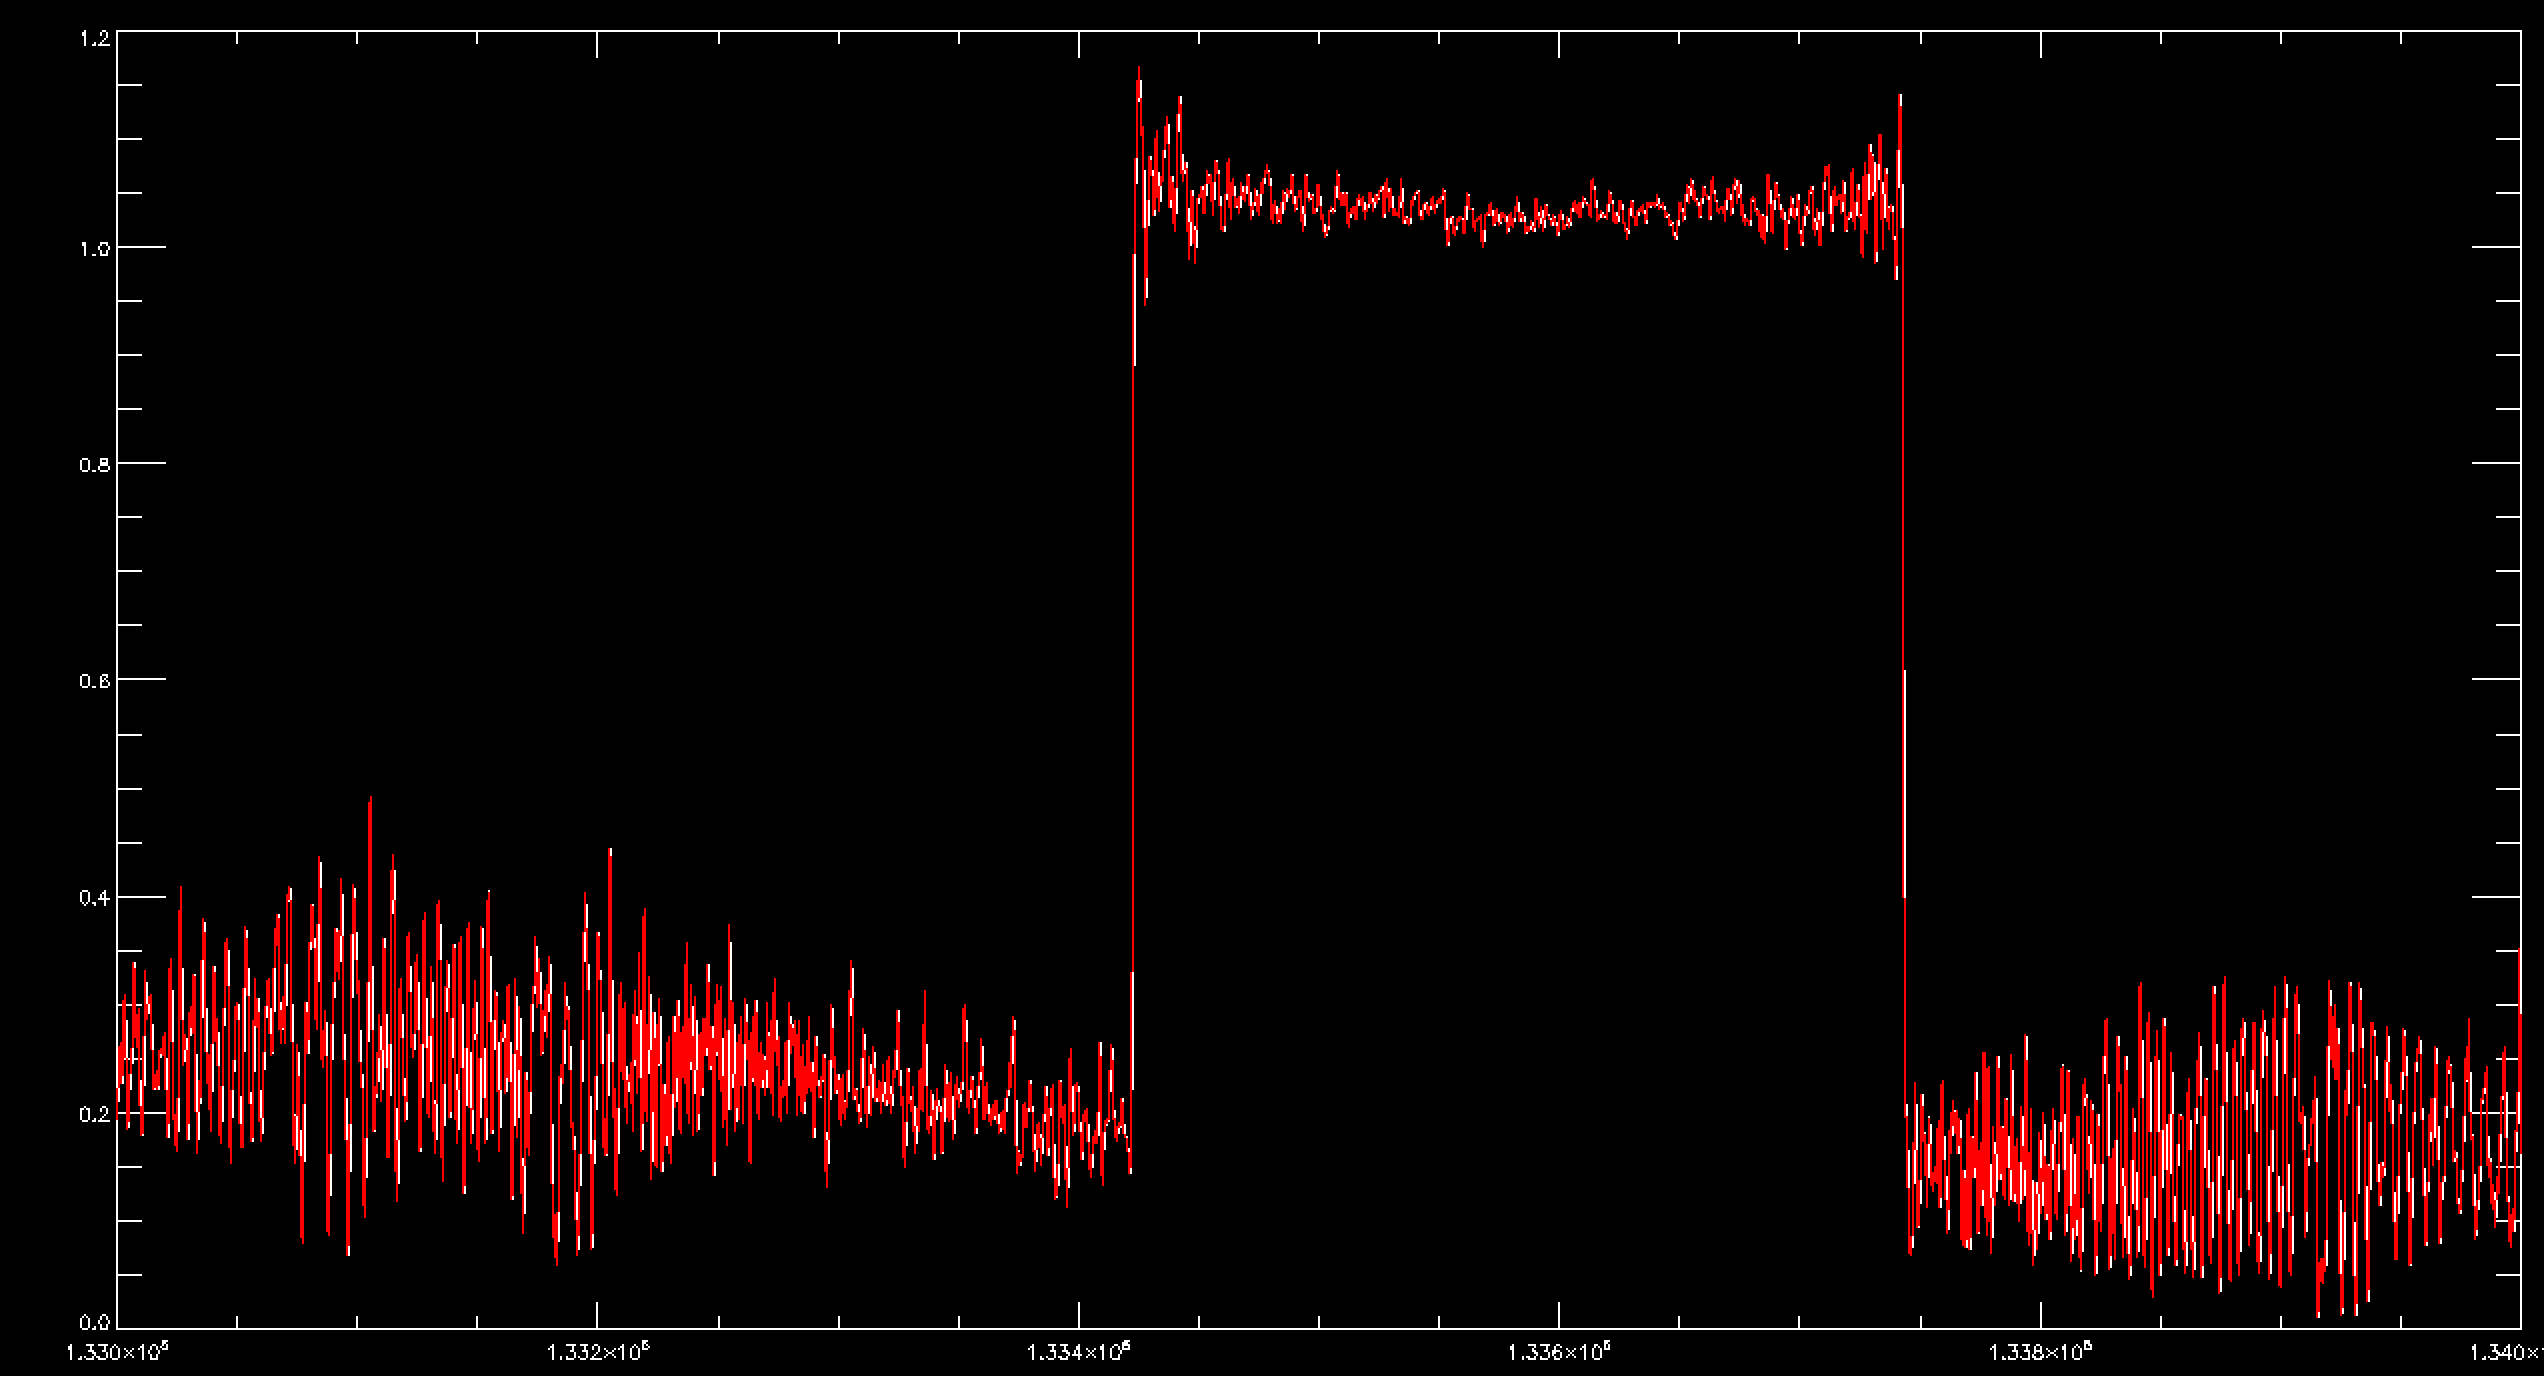
\includegraphics[width=\textwidth]{Encke_Gap}
    \end{subfigure}
    \begin{subfigure}[b]{0.32\textwidth}
        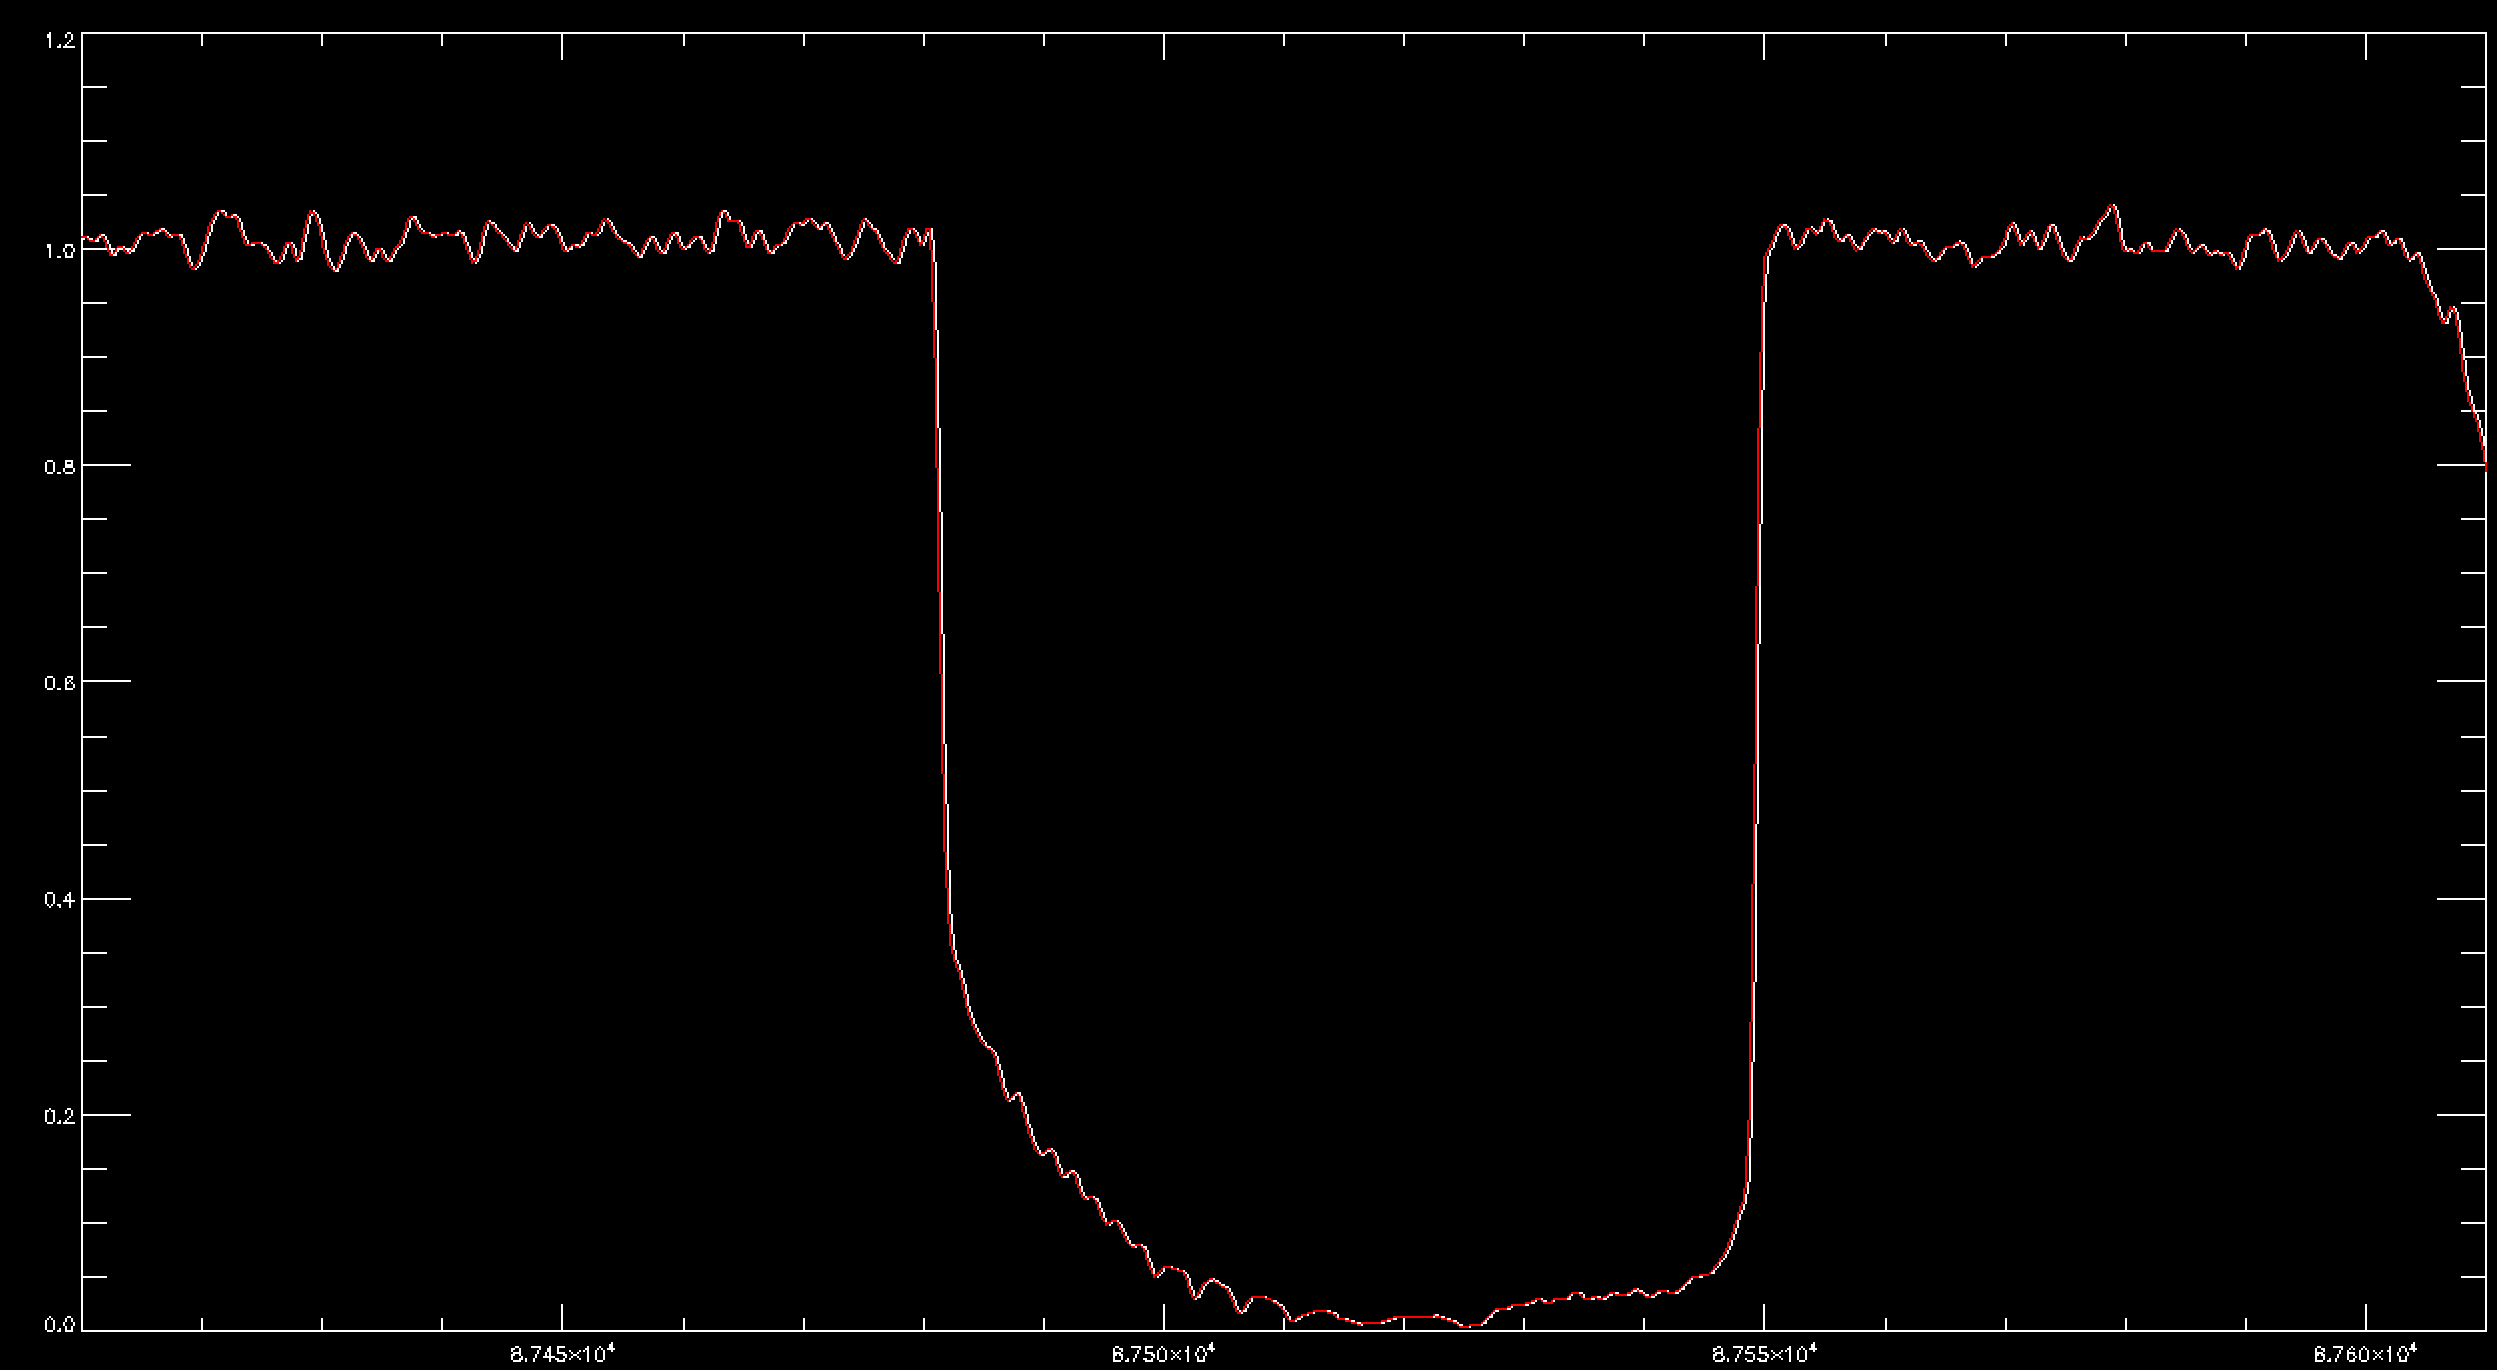
\includegraphics[width=\textwidth]{Maxwell}
    \end{subfigure}
    \begin{subfigure}[b]{0.32\textwidth}
        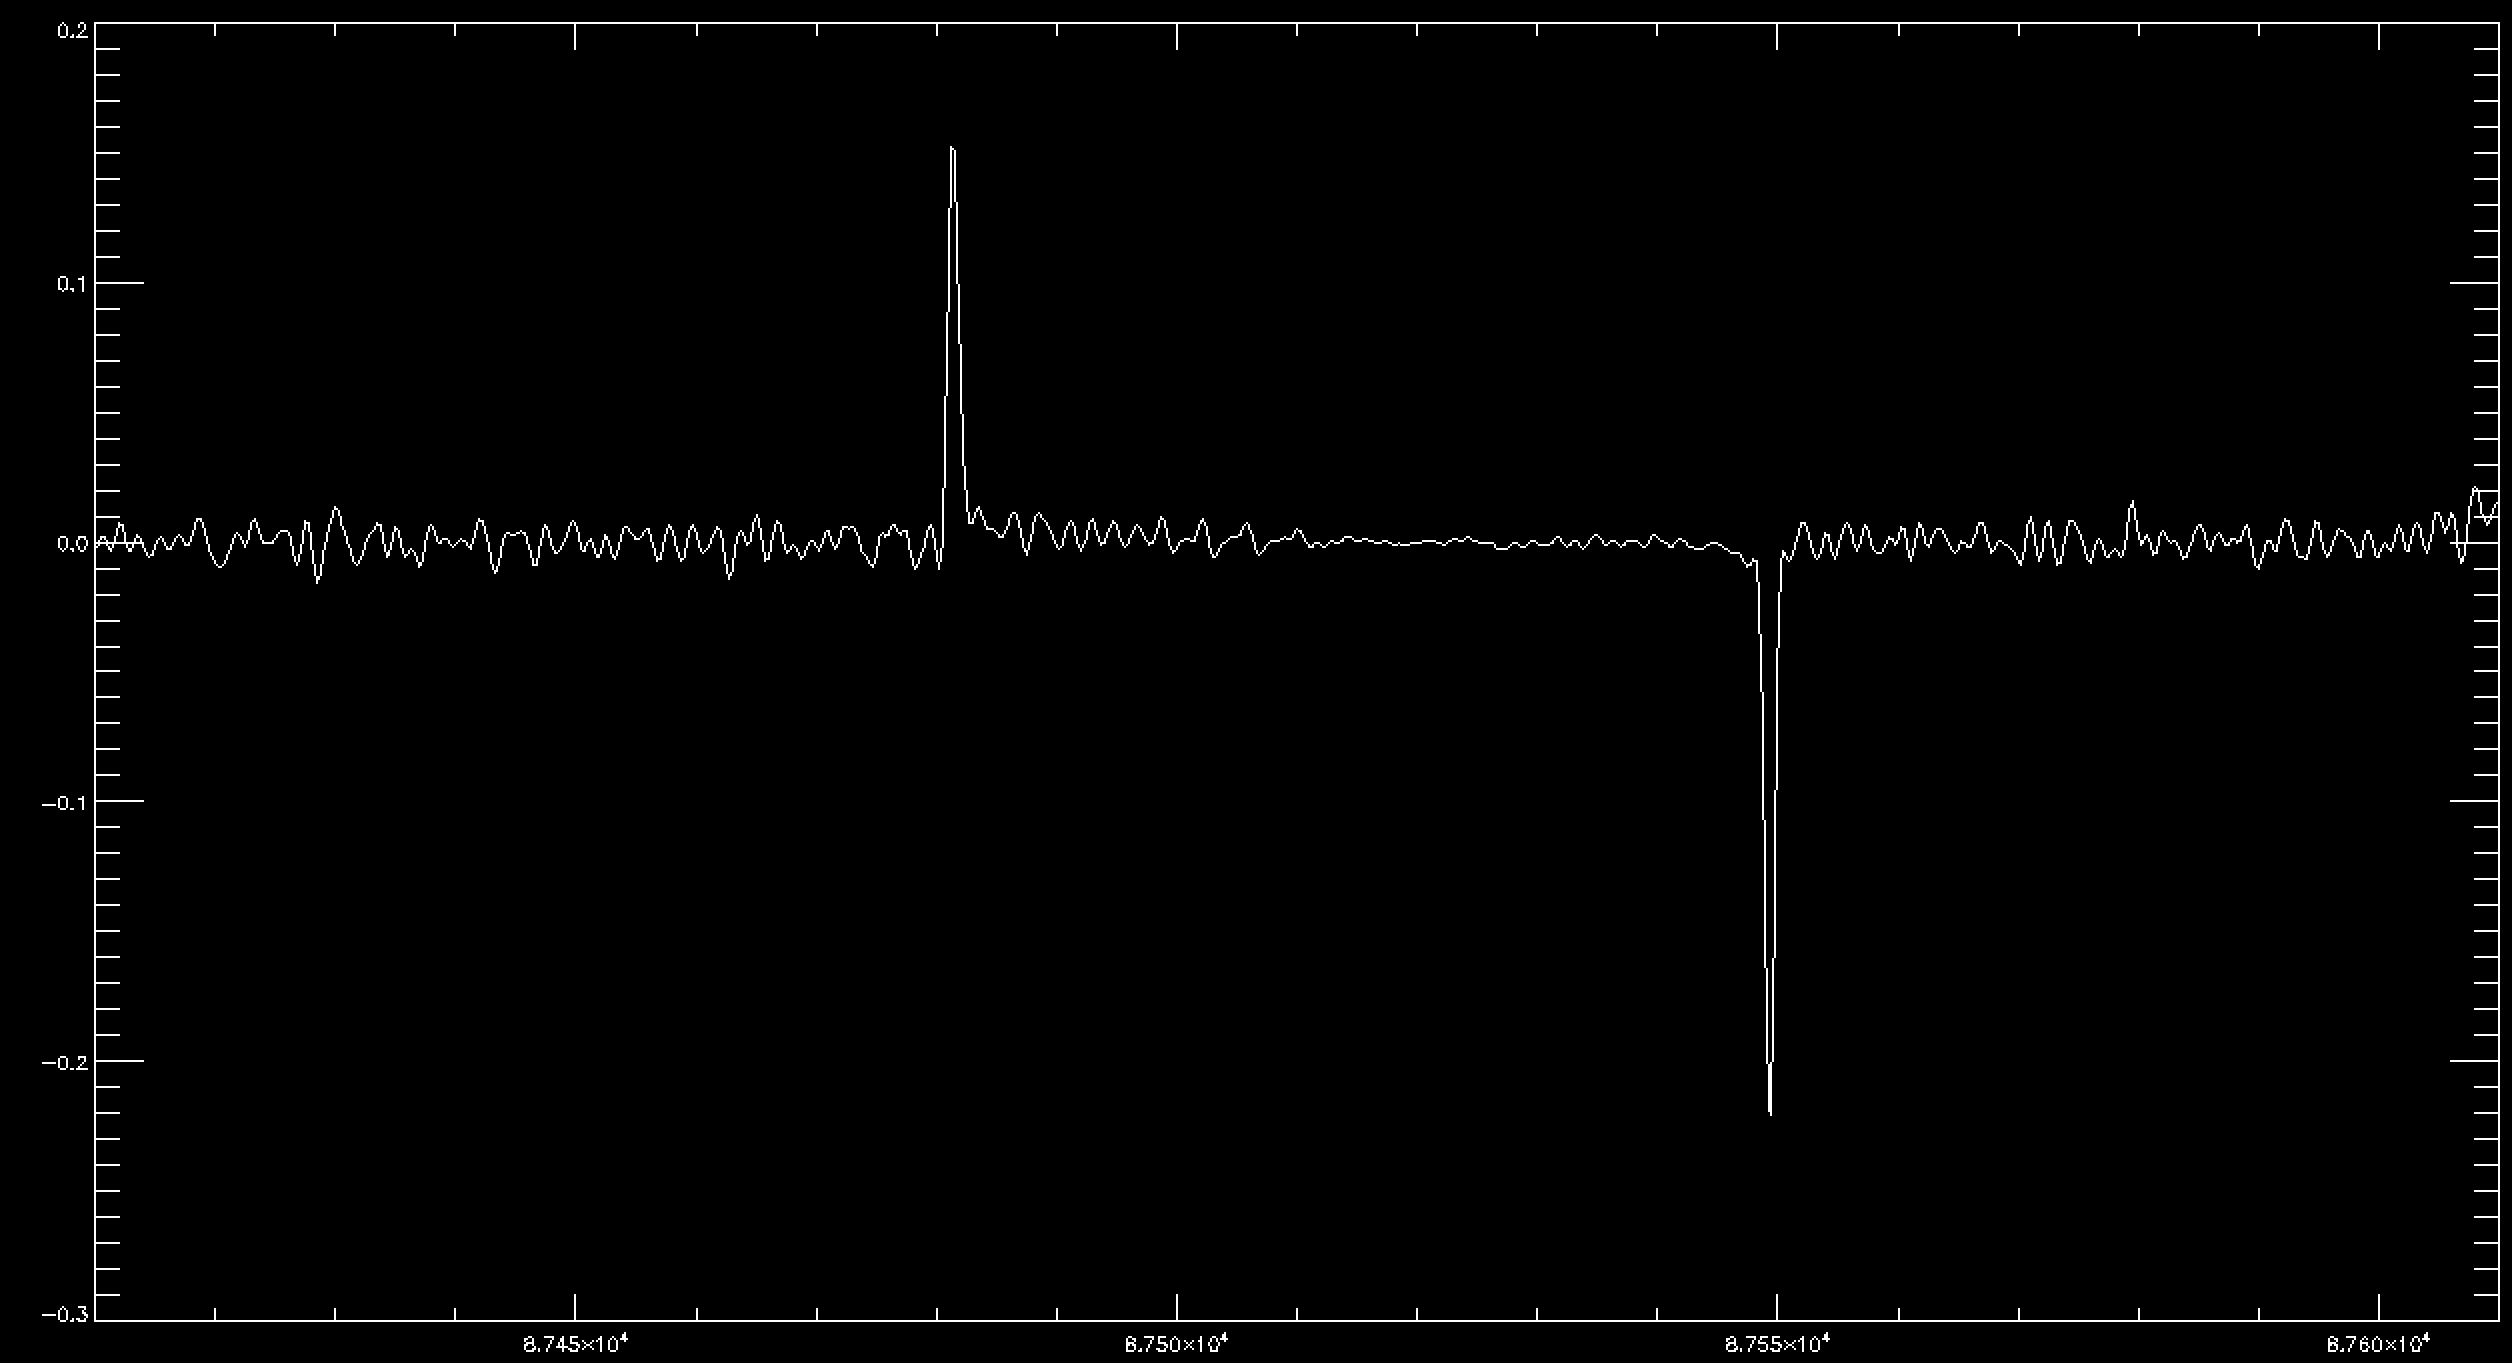
\includegraphics[width=\textwidth]{Maxwell_v4-v5}
    \end{subfigure}
\end{figure}
Thanks for this promising update. Could you plot the difference between v4.1 and v5 after you shift by one bin? I'd like to see how big the difference is at that point. I'm sure it will be possible to track down the off-by-one error at some point. 
All of this suggests that the FFT part of the code is very fast compared to the computation of Psi, which probably accounts for the TOTAL version being comparably fast or even faster - in a way, that's really good news, since it means that we can simplify the production code by using the Matched Filter everywhere. PS Jolene is going back to the old Rev7 inversions for the interim report, since that is what gave the best agreement with Essam before changes to the normalization. You should check with her to see what versions she's using. The Titan ringlet is a special case, since Essam is using 100 m and 1 km  and 10 km inversions - whatever you have in hand that gives the best match to his is what we should use for the report, but we need to include in our ISSUES AND CONCERNS notes on our team meeting notes pages that we'll need to resolve all of this eventually. Glenn is working on a Python spline routine, and I think we should defer until we are in the Python coding stage our final choices of normalizations. -Dick
Below is v4.1 vs v5 with a 250 meter shift. They are practically identical. Below that is the difference of v4.1 and v5 with a 250m shift (1 bin). -Ryan
\begin{figure}[H]
    \centering
    \begin{subfigure}[b]{0.49\textwidth}
        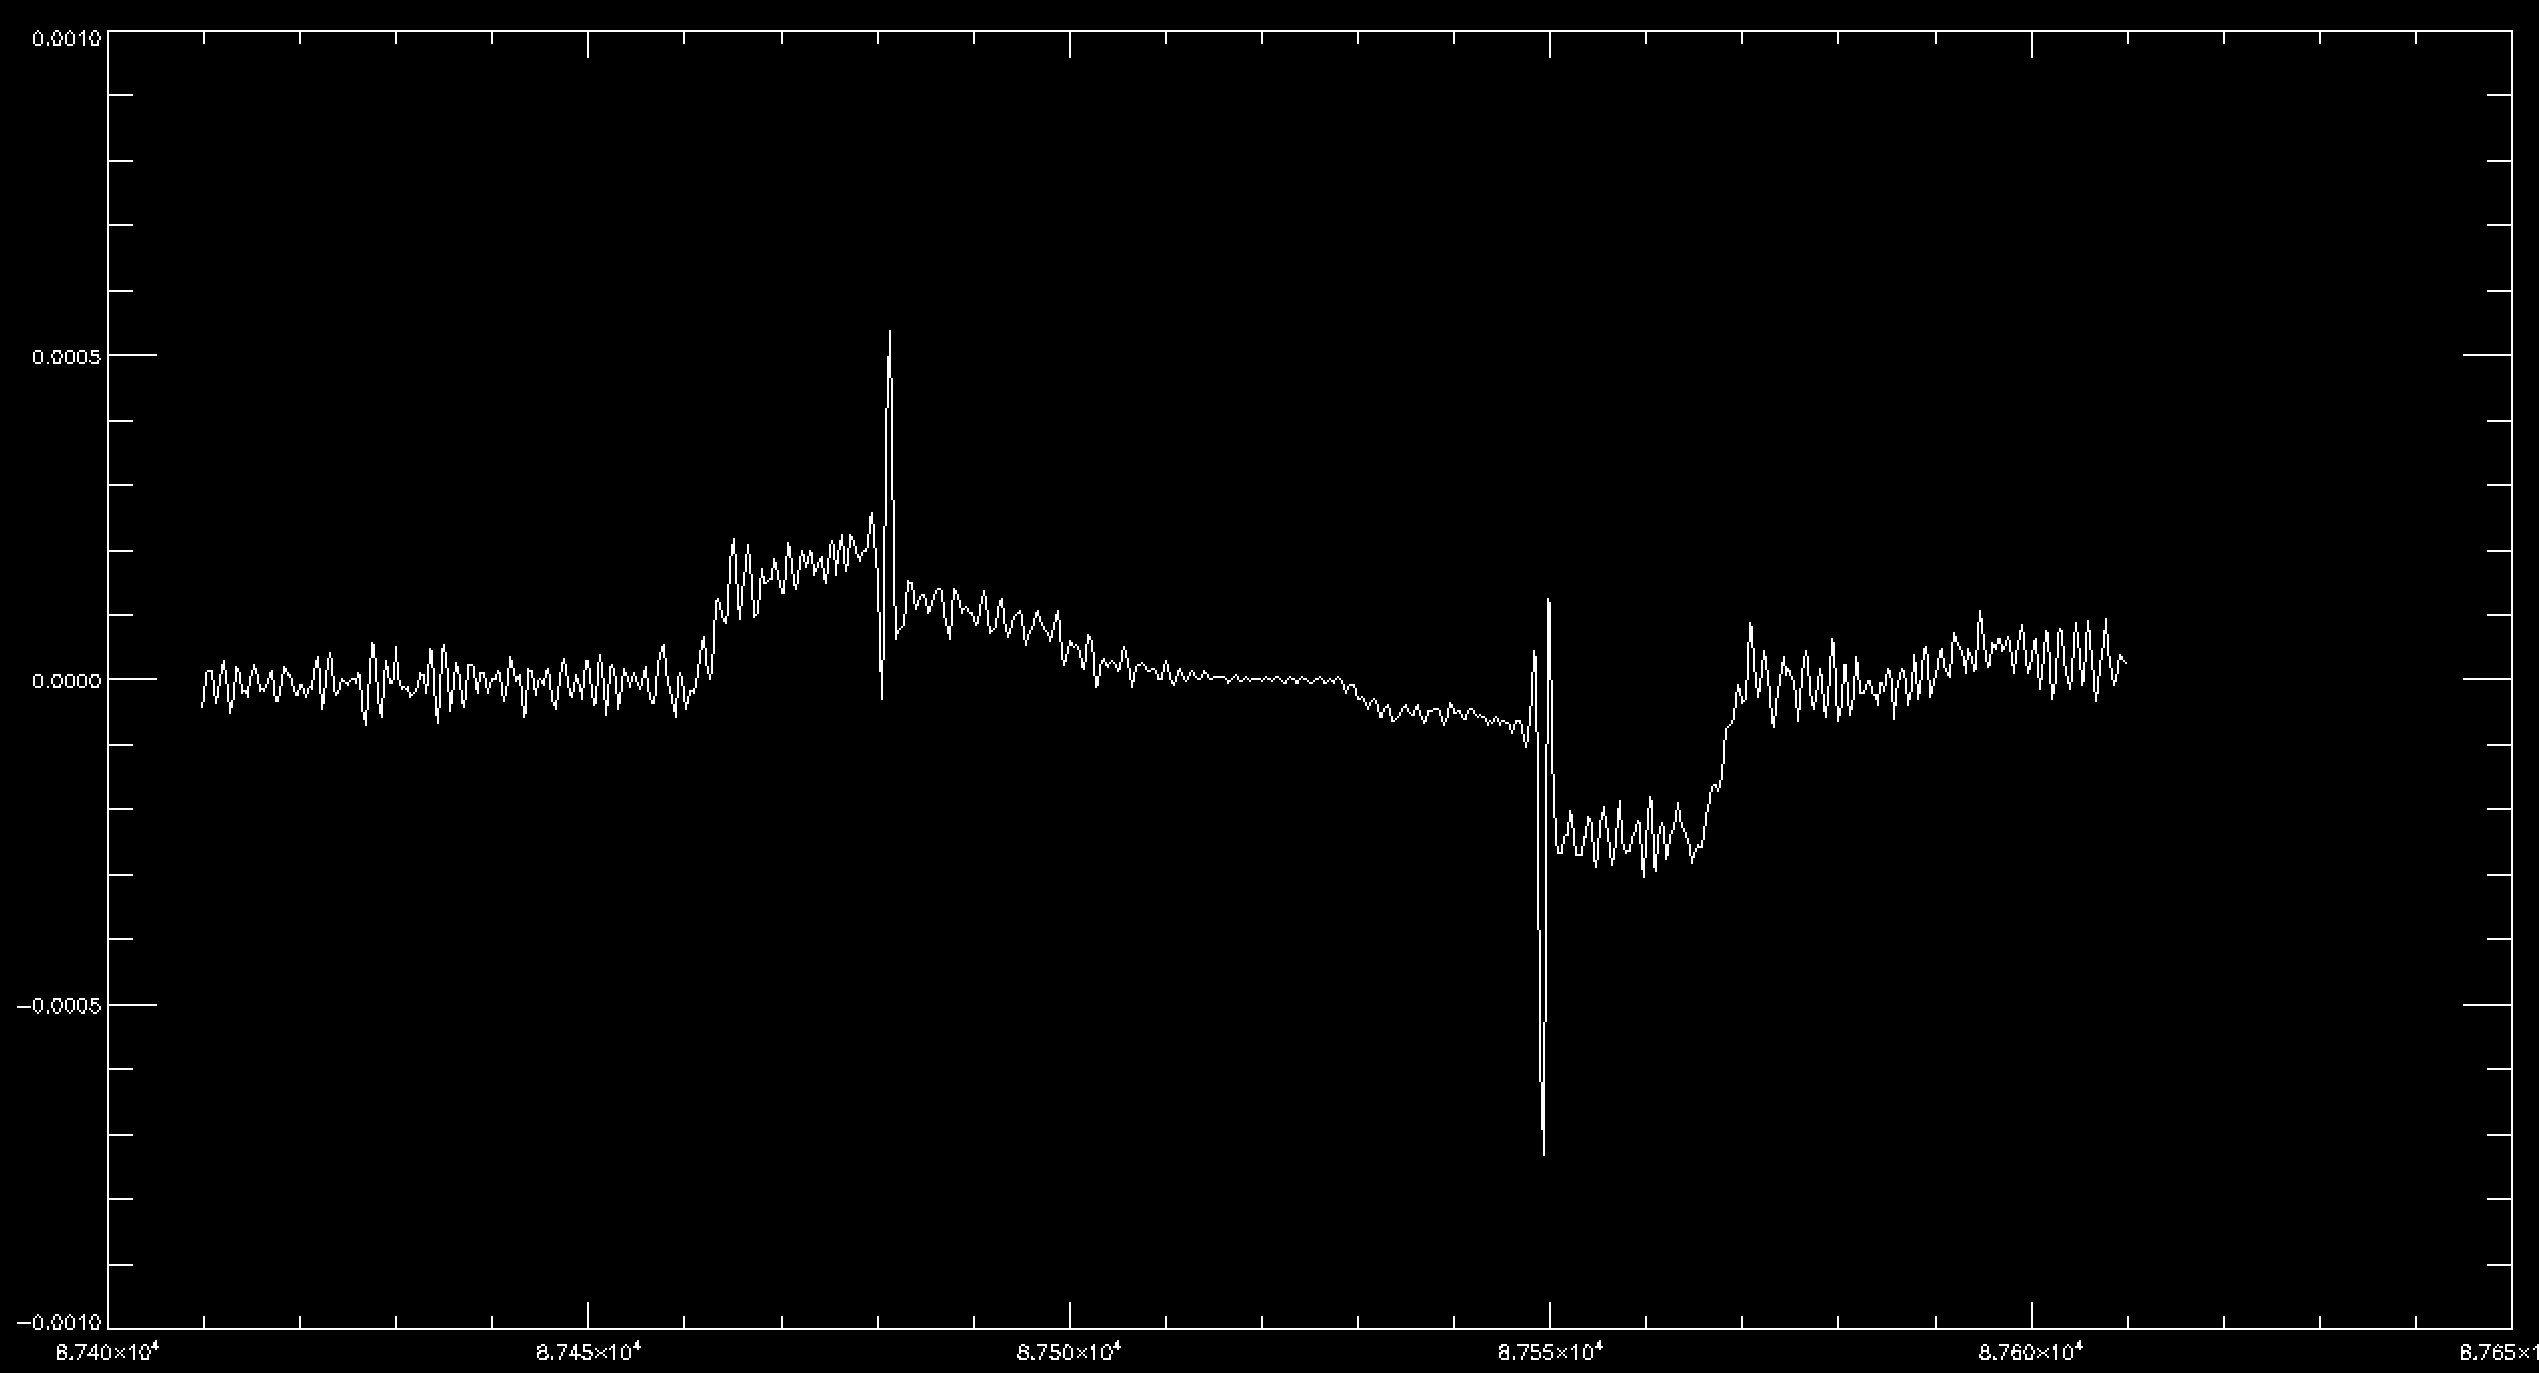
\includegraphics[width=\textwidth]{Maxwell_1_Bin_Shift}
    \end{subfigure}
        \begin{subfigure}[b]{0.49\textwidth}
        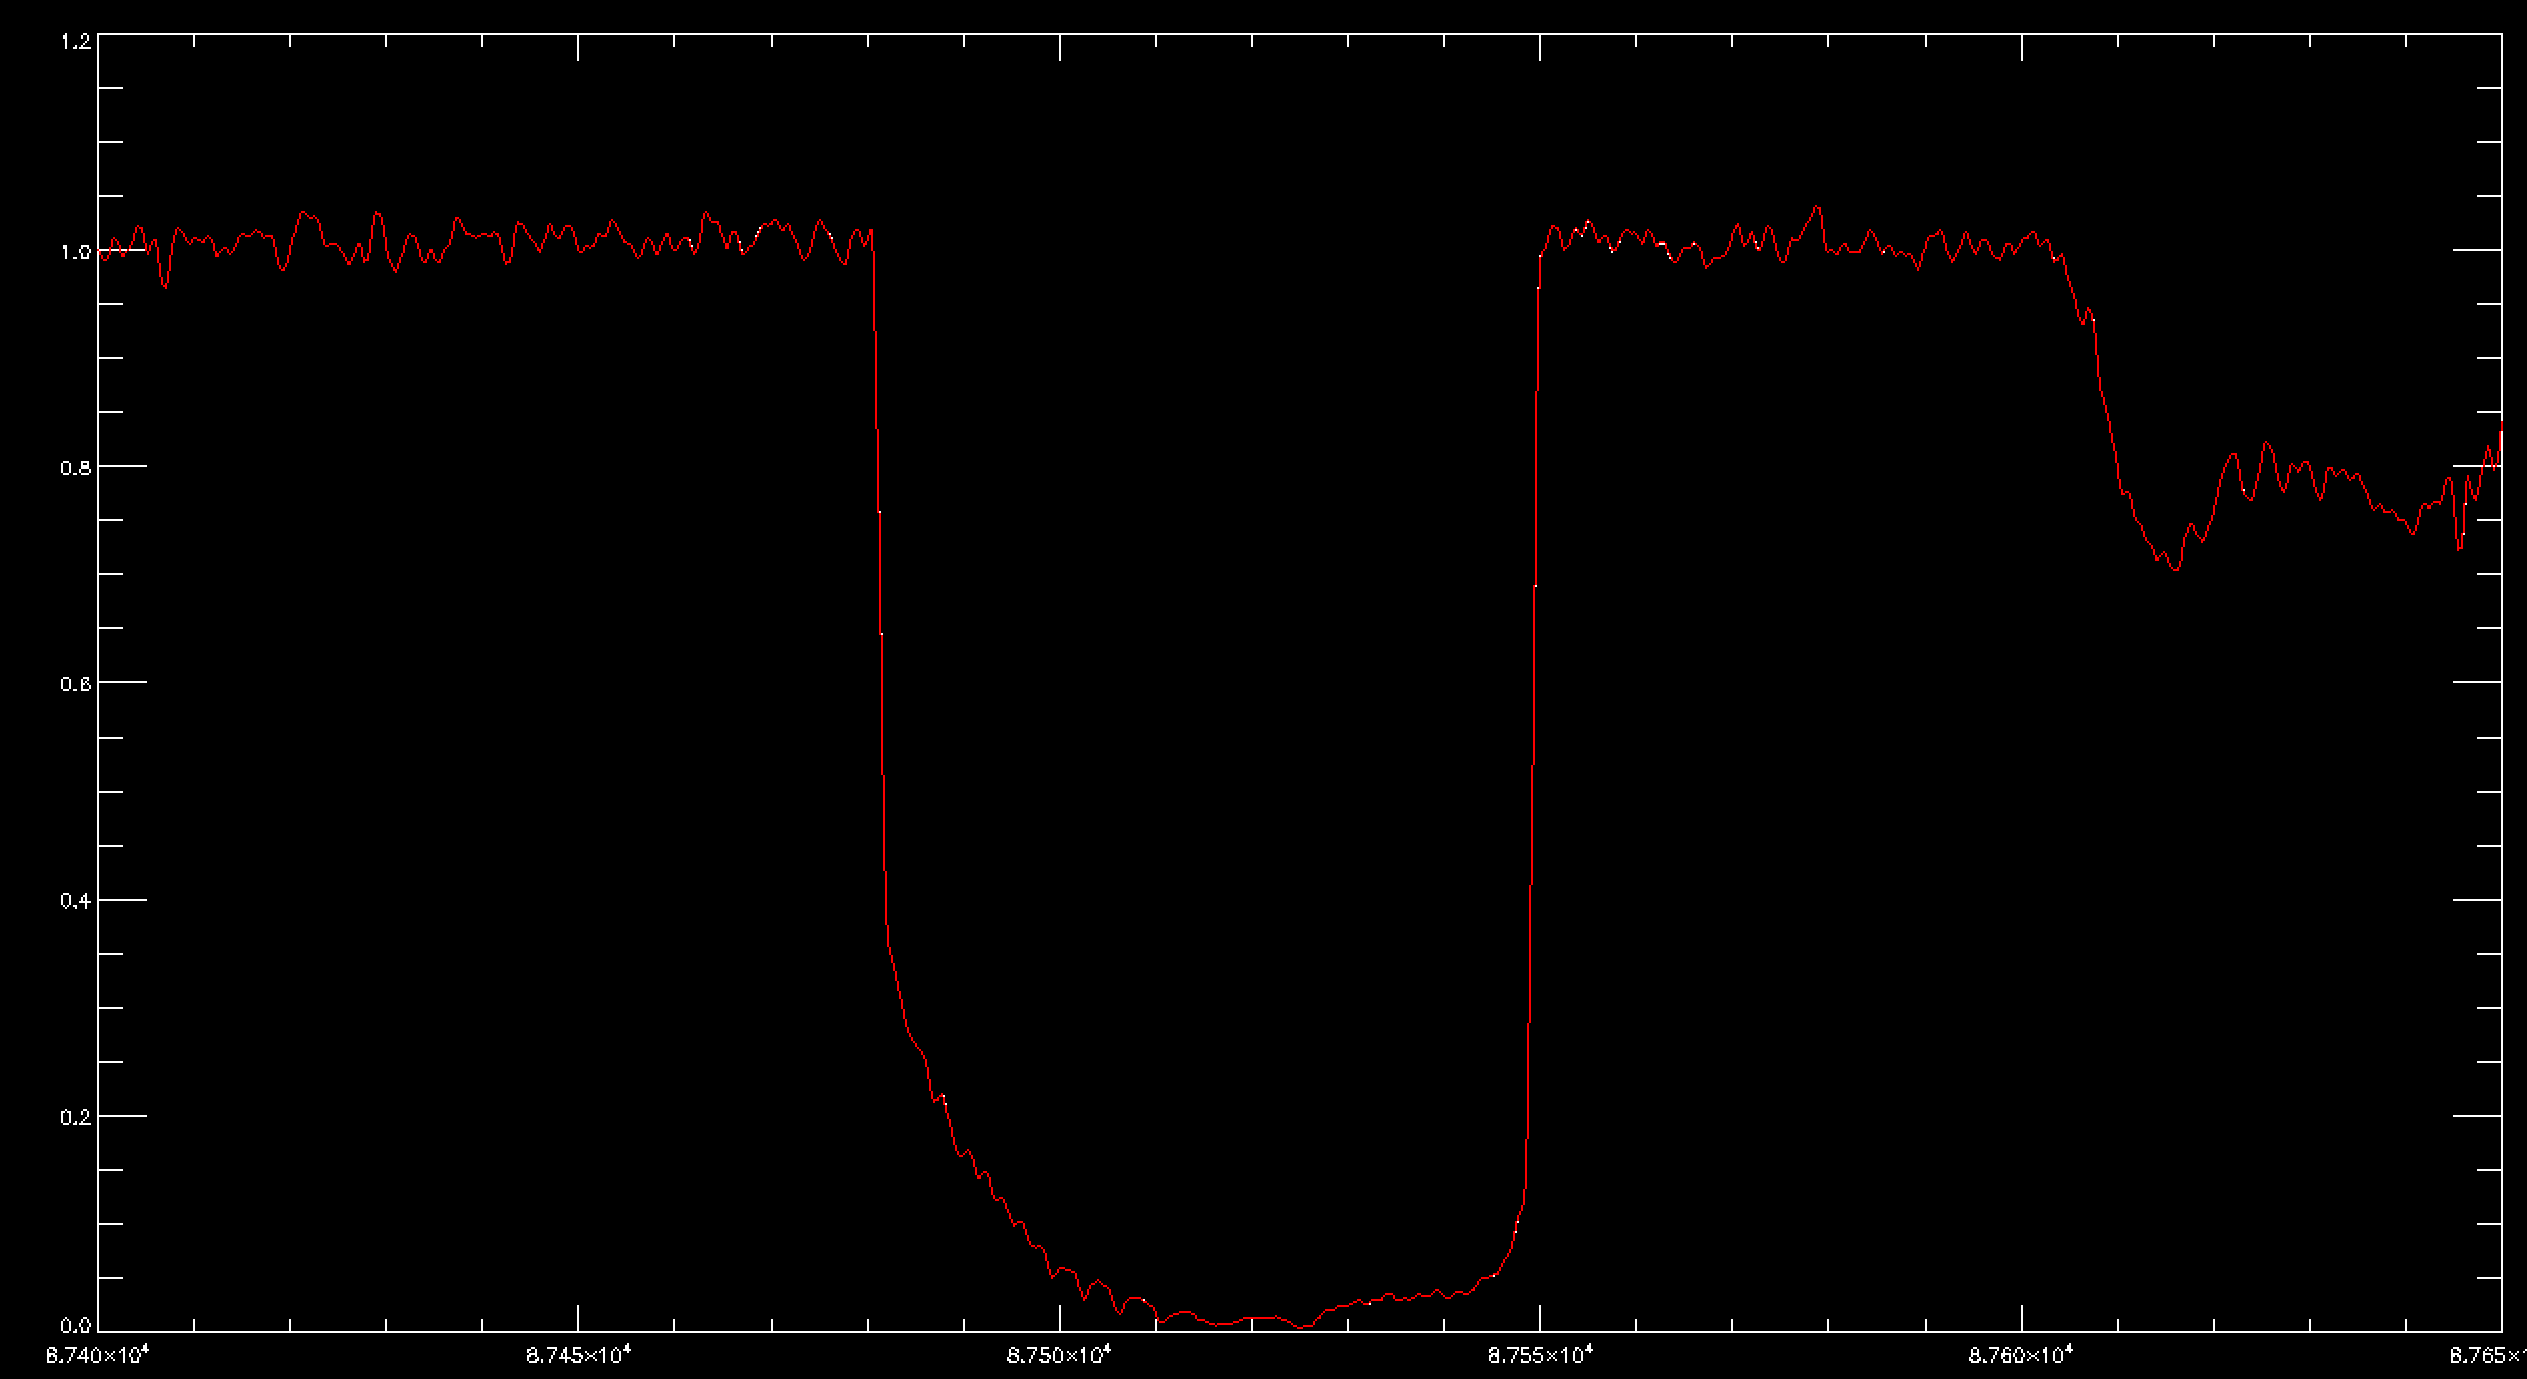
\includegraphics[width=\textwidth]{Maxwell_250m}
    \end{subfigure}
\end{figure}
Thanks, Ryan - They do indeed look very similar! Once the off by a bin origin gets identified, I think we might want to continue to use the straightforward integration version - do you agree? It will be easiest to document, and we won't need users to install FFTW. By the way, what is the window width compared to the width of the ring? What do you make of the inverse symmetry about the midpoint of the lower plot - if you invert the RHS and fold it about the middle, the two curves look almost identical. I'd like to understand the origin of that pattern, if possible, even though it is below the level of practical significance. Could it be related to a slightly different way in which the window is centered in the two calculations? If you use Essam's savefile for Rev007E and his normalized diffraction pattern, how well do your two methods (V4.1 and V5) compare to his diffraction-corrected profile? Could you plot up that difference? I'd like to include that in our interim report in some fashion. -Dick\\
My guess is that the shift is not quite 1 bin, but 1.1 bin or something like that. That up-spike down-spike seems reminiscent of the offset we had back in November. -Ryan\\
One possible way to resolve this would be to do a forward and inverse problem for a translucent ring of a given optical depth and to compare the V4.1 and V5 results with the expected results from an analytic solution. That's how I usually try to track down finicky offsets like this - to try to reproduce a result with an analytic solution. (The one you did using Fresel integrals.) -Dick\\
v4.1 is doing the shifting, not v5. I compared the two with Essams files:
\begin{lstlisting}[language=bash]
../../../../data/RSSringoccs/savefiles/RSS_007E_X43_23MAR09.sav
\end{lstlisting}
-Ryan
Ok, that's good to know. Does that mean that V4.0 was shifting as well? Could you send me plots of the V5 comparison with Essam's result? -Dick\\
Final update for the night: I ran res\_char with v5, and using the optimal resolution gave a max error of 0.3\%. If you recall, v3 had a 2\% maximum error (The L\_infinity norm). The error is now on the same order of magnitude as the v4.1 vs v5 max error, which is also promising. The optimization code ran at 50m intervals, I'll use a finer interval to try and home in on sqrt(2), see where the best one is. I'll Have finalized plots ready for tomorrow morning, and you can do the IDL plotting magic. Just got your message, I'll make the plot comparison for v4.1 and v5 now. v4 used and even number of points per window, and v4.1 uses an odd number of points, so I believe this shifts the bin over, explaining the discrepancy between v4 and v4.1. v4.1 and v5 both use odd, so I don't know where the shift comes from there. Here you are. The first one is v5, and the second v4.1. Once v4.1 is shifted, the max error is 0.38\%, still better than before. -Ryan
\begin{figure}[H]
    \centering
    \begin{subfigure}[b]{0.49\textwidth}
        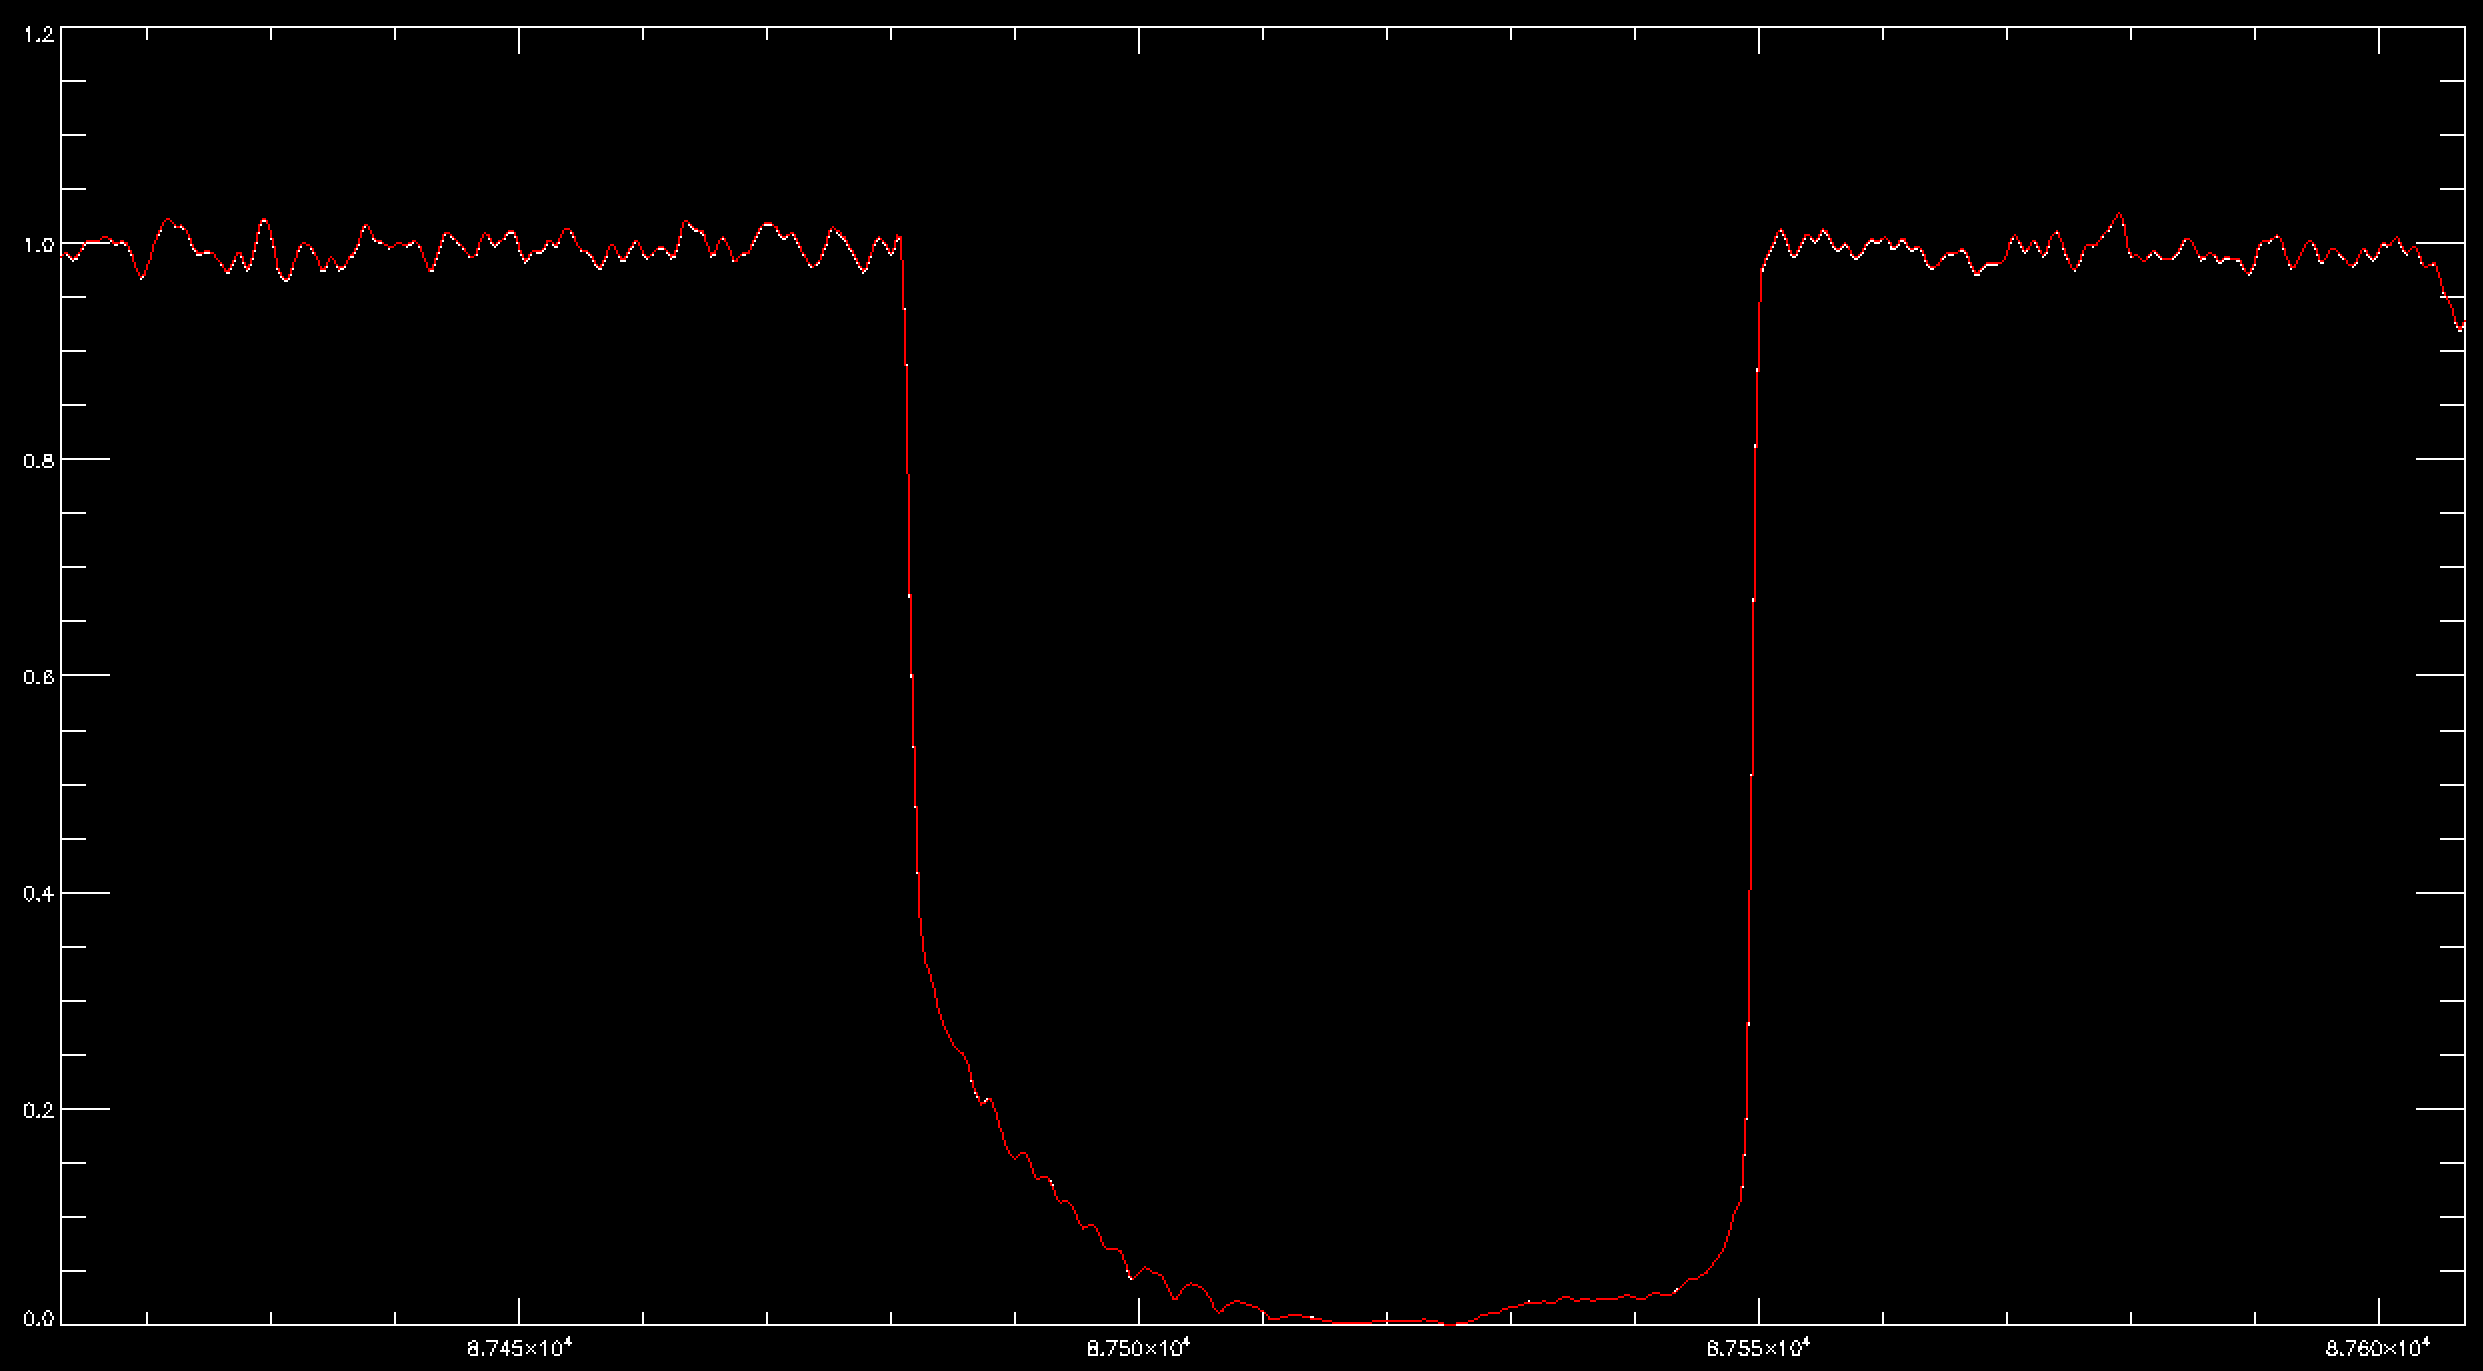
\includegraphics[width=\textwidth]{Maxwell_Our_Geo_Essam_Data}
    \end{subfigure}
    \begin{subfigure}[b]{0.49\textwidth}
        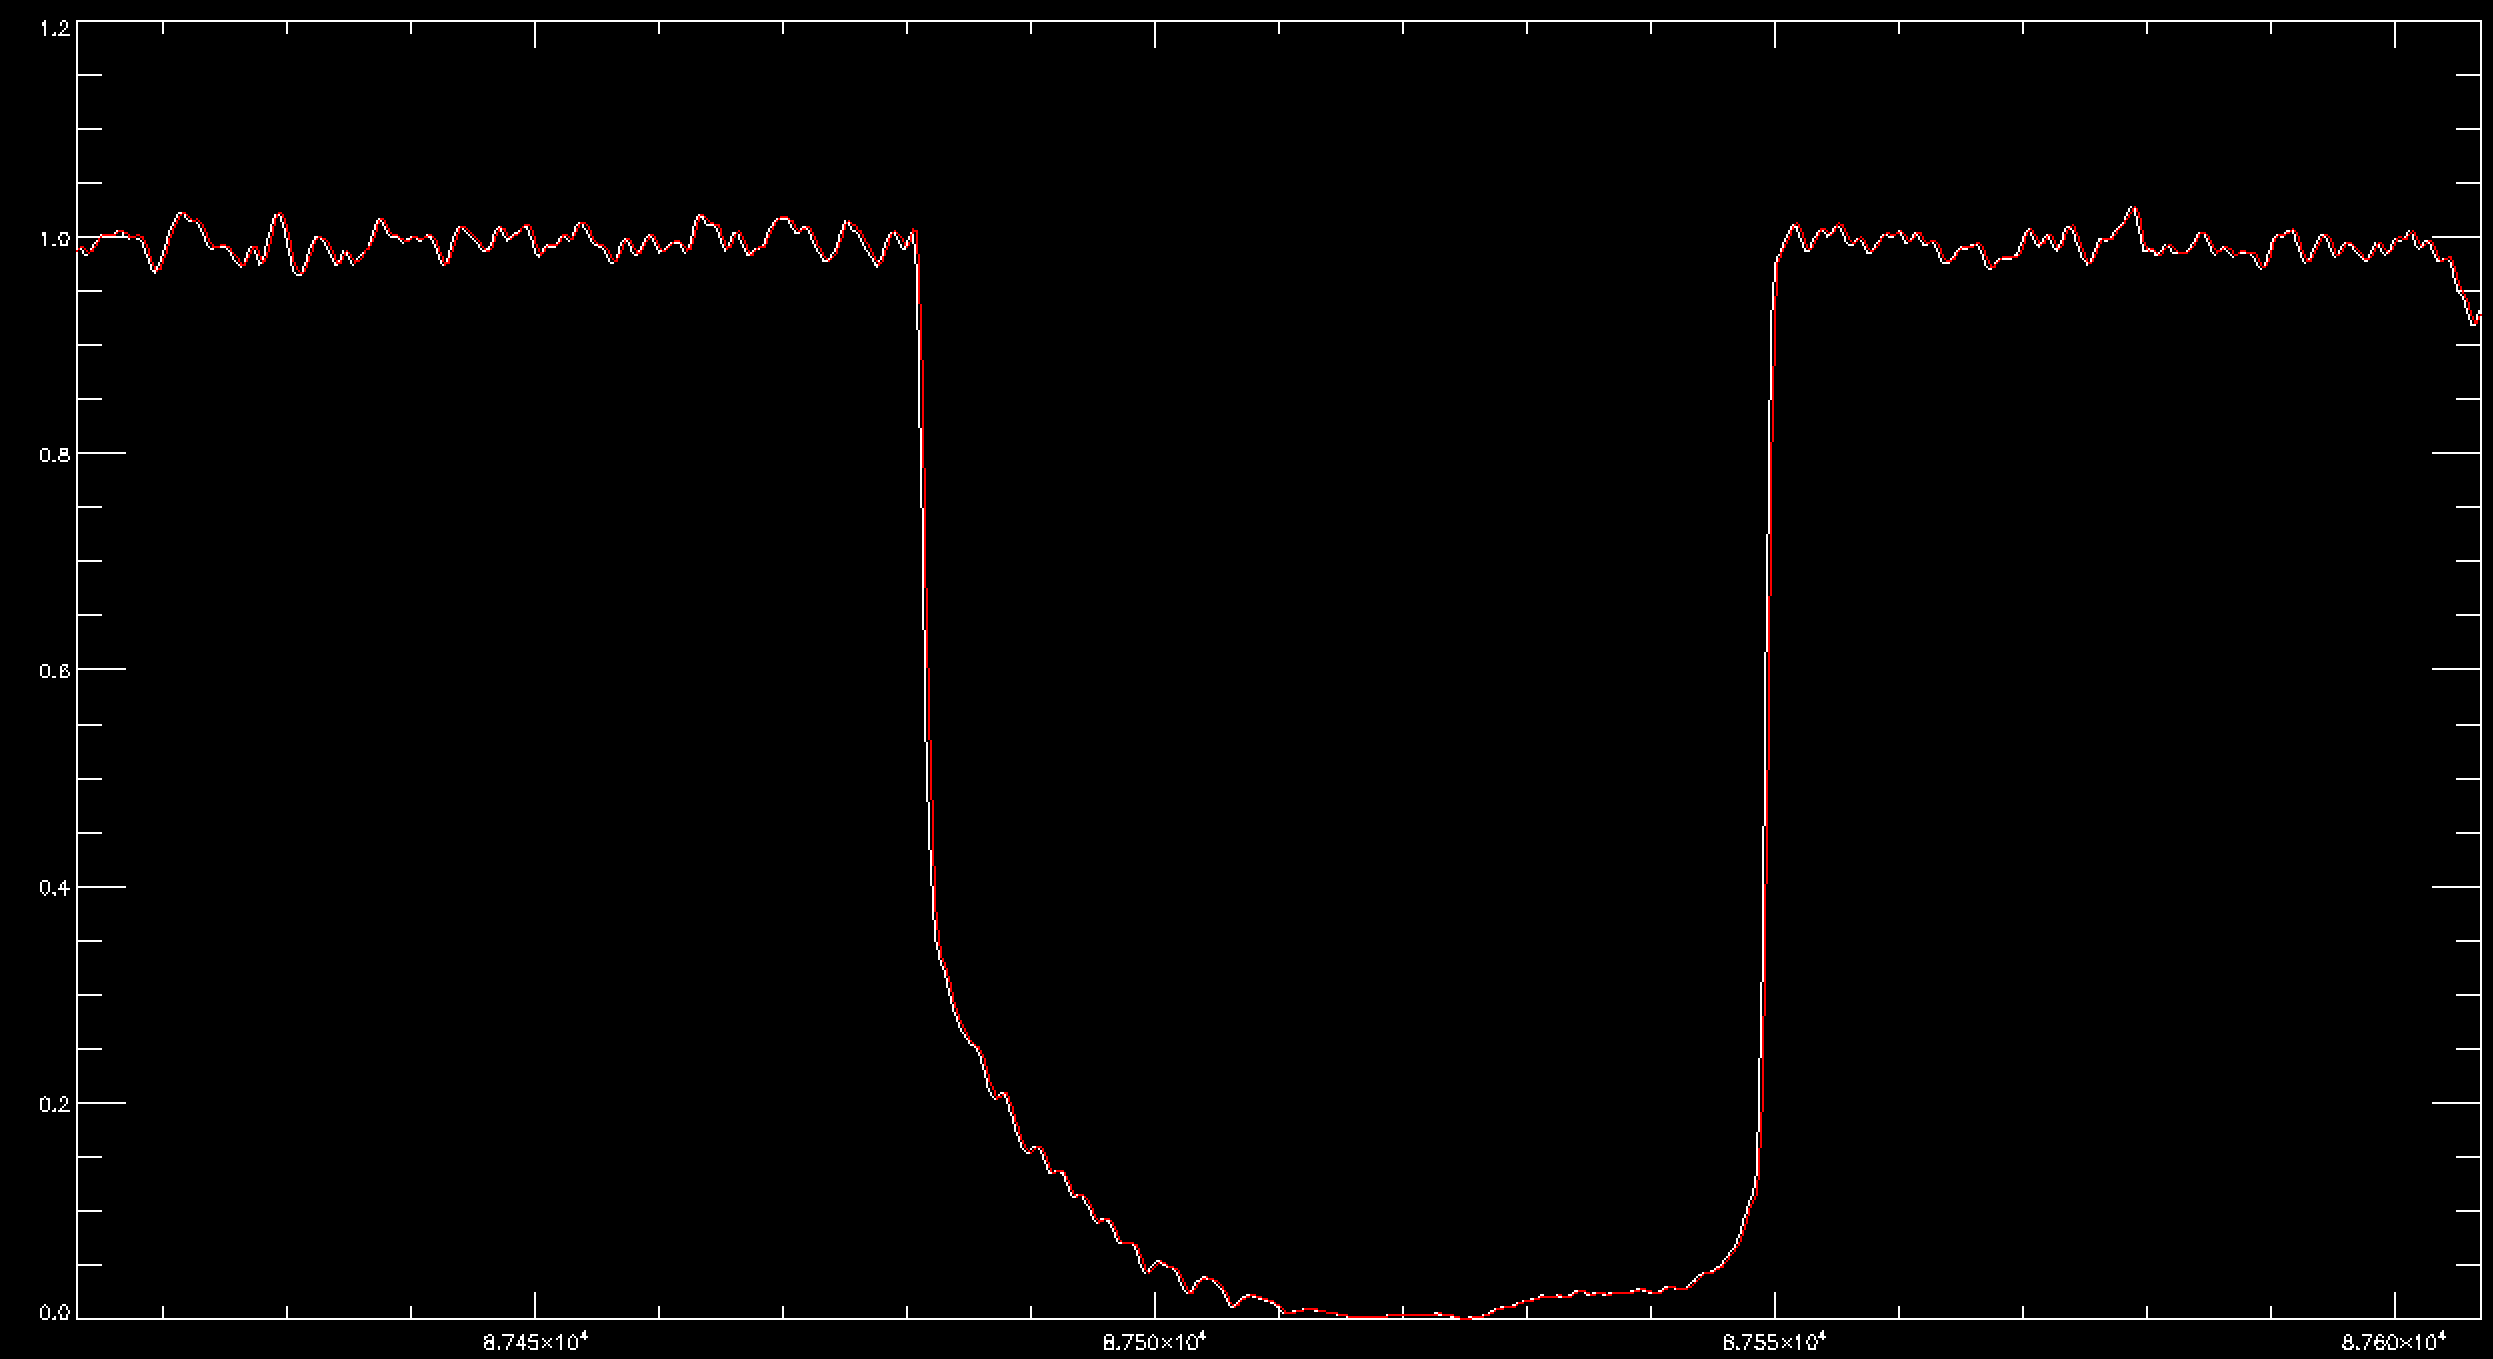
\includegraphics[width=\textwidth]{images/Maxwell_v4_1.png}
    \end{subfigure}
\end{figure}
Great - I'll be interested to find out what scale factor you applied to W. By the way, I think we discussed the possibility that this scale factor might be variable across the rings -- or not. Either one would help us diagnose the difference between Essam's approach and ours in defining $\Delta R_{\rm eff}$ -Dick
\subsubsection{\footnotesize RE: Titan Ringlet Plots}
Hi, Ryan - When you have a chance would you send me a plot (and location of plotting program) that does your best reproduce Essam's Titan ringlet plots for Rev007E from the User's Guide (100m, 1 km, and 10 km resolution)? 
Also, could you process the F ring profiles Glenn did (rev 123 or rev 125, S, X, Ka) at 100-m resolution? He may need to supply you with 50-m resolution files. -Dick\\
There is a code that uses v5 to make plots and compare with Essam, using Essam's data:\\
/Volumes/dione\_raid2/Research/TC2017/rmaguire/v5/compare/rjm\_diff\_corr\_compare.pro
The inputs are at the top of the code:
\begin{itemize}
    \item WType - Only 'kb25' or 'kbmod' are allowed for simplicity.
    \item range = [start,end]
    \item res\_km - a double for resolution, in kilometers.
\end{itemize}
At the bottom of the code is the filename you wish to save the output as:\\
save, r, tau\_tc, power\_tc, power\_vals\_EAM, tau\_norm\_vals\_EAM,\$\\
filename = 'comparisons/2018\_01\_24\_rev007\_E\_X43\_Essam\_Comparison\_Maxwell\_Ringlet\_res\_1000m\_v5\_code\_2.sav'
\begin{figure}[H]
    \centering
    \begin{subfigure}[b]{0.49\textwidth}
        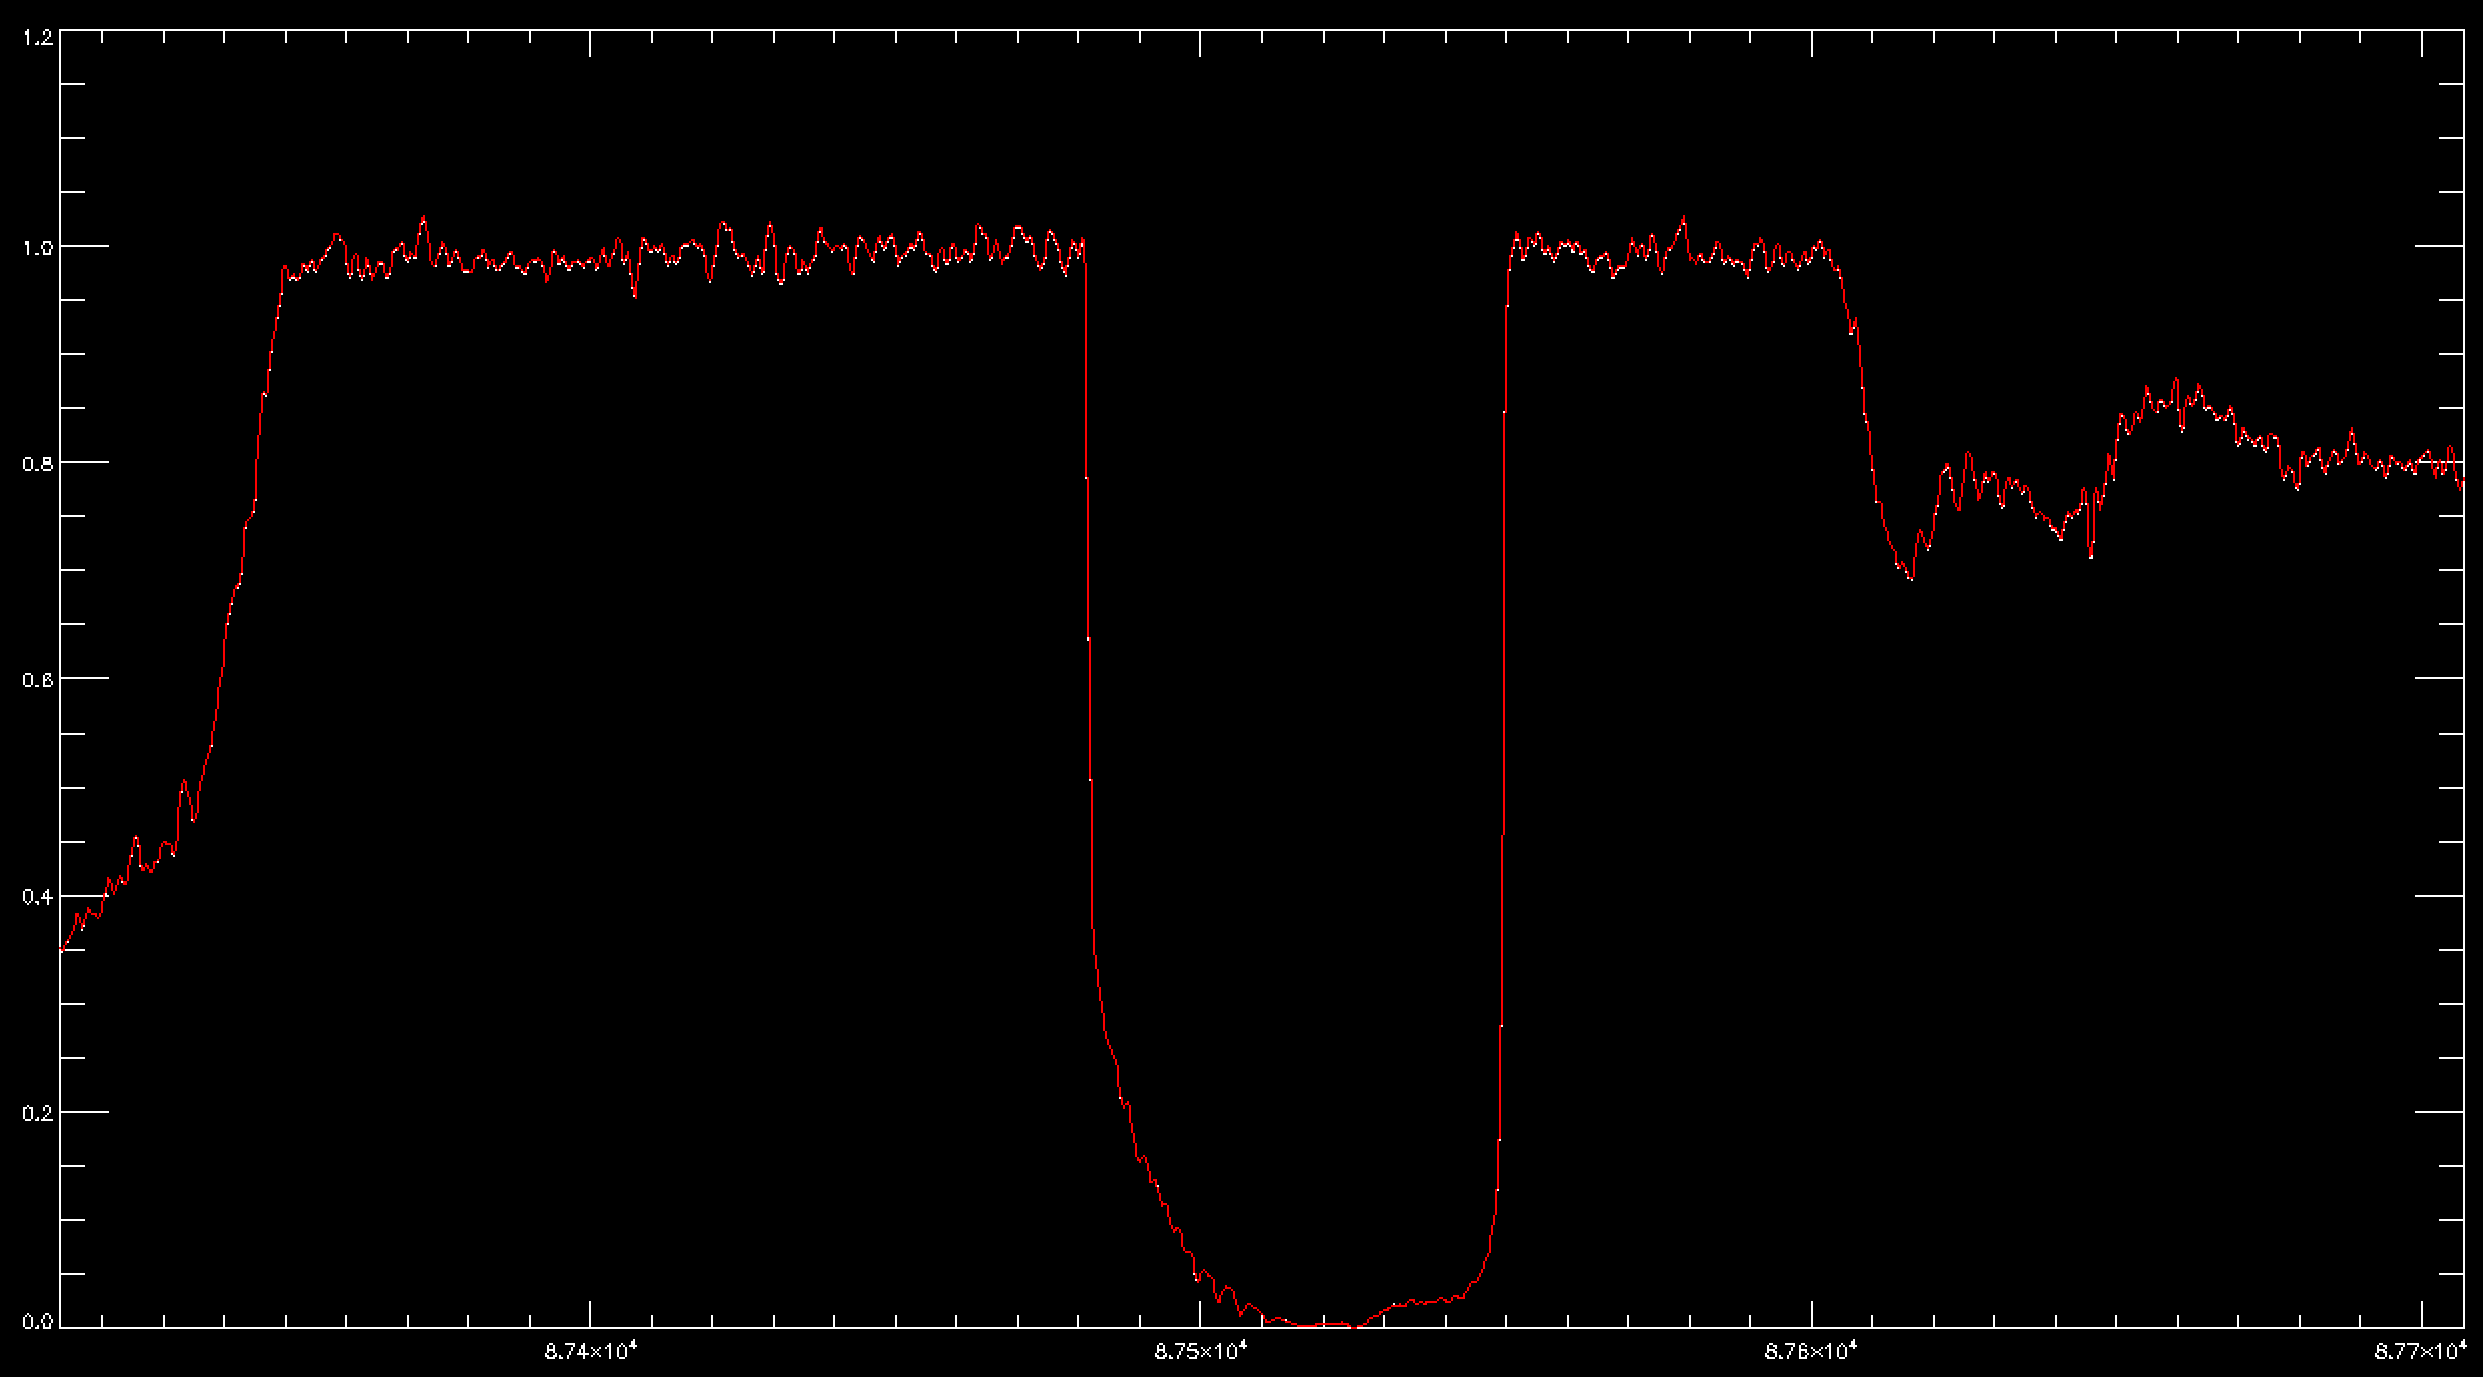
\includegraphics[width=\textwidth]{Maxwell_v5}
    \end{subfigure}
    \begin{subfigure}[b]{0.49\textwidth}
        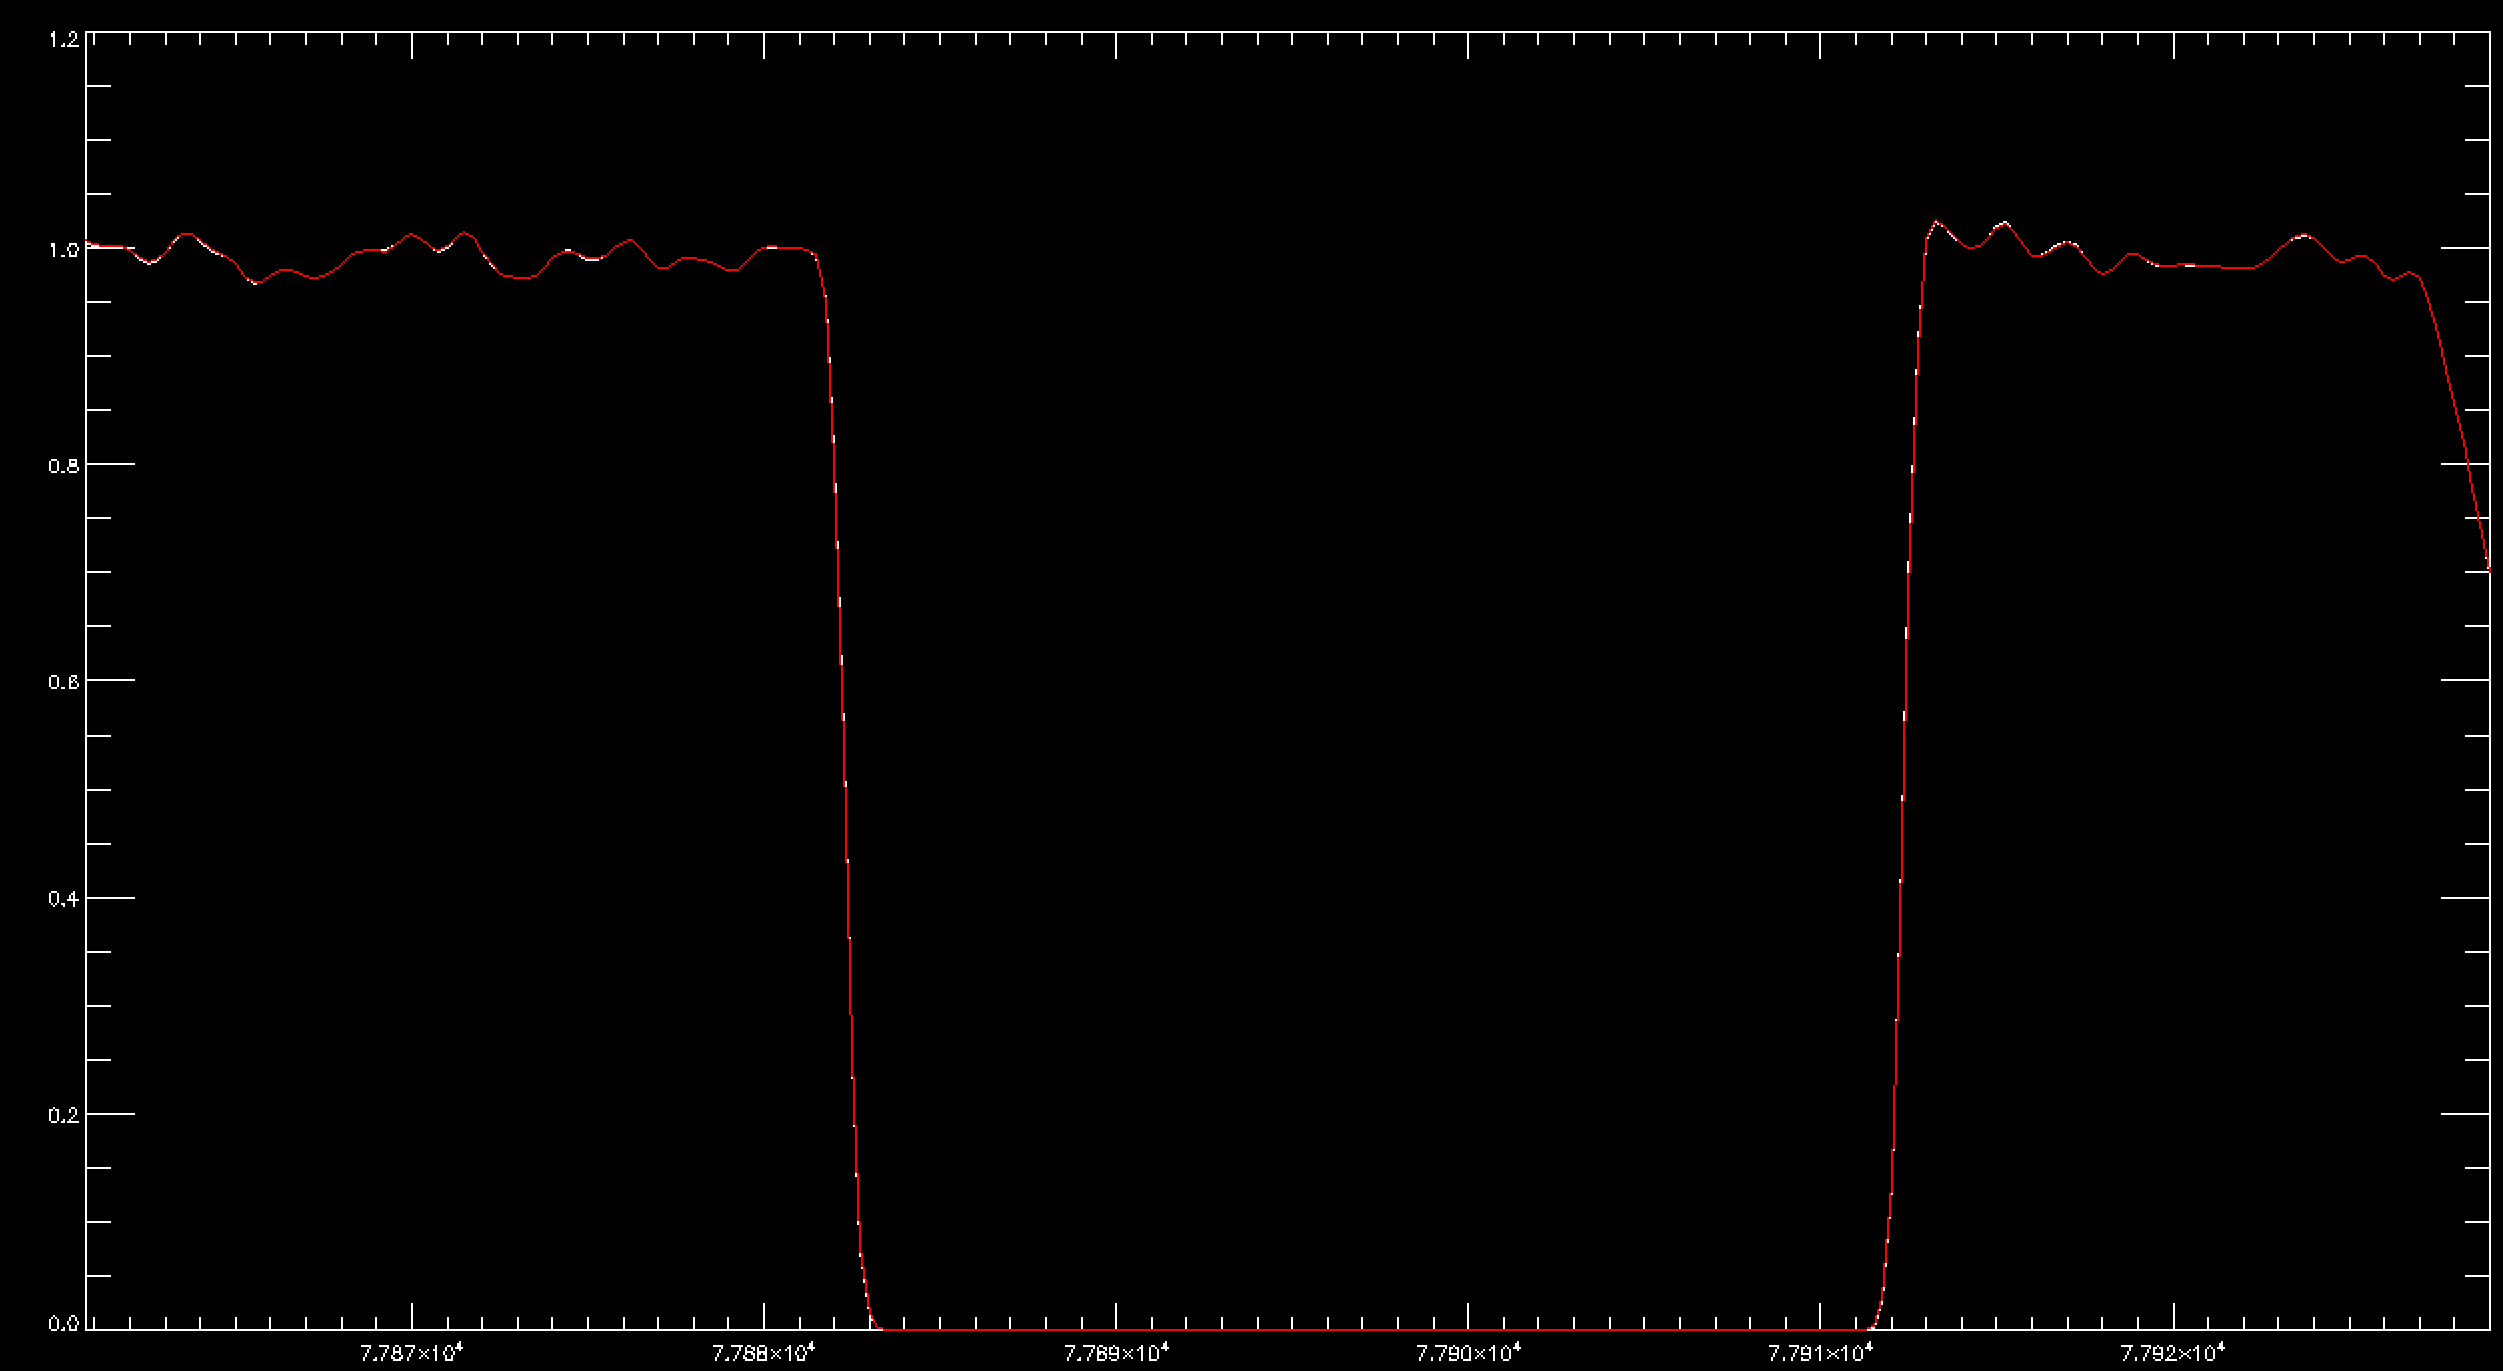
\includegraphics[width=\textwidth]{Titan_v5}
    \end{subfigure}
\end{figure}
tau\_tc, power\_tc, power\_vals\_EAM, tau\_norm\_vals\_EAM are now saved at:\\
/TC2017/rmaguire/v5/compare/comparisons/2018\_01\_25\_rev007\_E\_X43\_Essam\_Comparison\_Maxwell\_Ringlet\_res\_1000m\_v5\_code\_2.sav\\
/TC2017/rmaguire/v5/compare/comparisons/2018\_01\_25\_rev007\_E\_X43\_Essam\_Comparison\_Titan\_Ringlet\_res\_1000m\_v5\_code\_1.sav\\
Jolene made modifications so that our v2 savefile is used with v5 reconstruction, and then compares with Essam:\\
/Volumes/dione\_raid2/Research/TC2017/rmaguire/v5/compare/rjm\_diff\_corr\_compare.pro\\
I haven't looked over the code, but she showed me the plots for the Maxwell ringlet and they looked very good. Yesterday I discovered that, due to large window sizes, the Riemann sum that is used in v5 cannot adequately capture the nature of the rapid oscillations that exp(ipsi) has. So rev-133 and rev-123 should use v4.1. For rev007, even at 100m resolution, the windows are small enough that the Riemann sum captures the same amount of detail as the FFT. I'm actually curious to find out what form of integration FFT uses. Last night I tried Simpson and Newton-Cotes integration, rather than just TOTAL, but both seemed rather poor for rev133. Also note, a quadratic fit to psi for the c-ring ripples is horrible. Indeed, a quartic fit was pretty bad ass well. A 6th degree polynomial fit incredibly well, however. The fact that psi can still be fit very well by a polynomial demonstrates why FFT works so well. I will make a v4.1 version of this compare program now. Should be done soon.
\subsubsection{\footnotesize RE: Updates 01/26/2018}
I'm going to make an updated version of that compare program and add the figures to the interim report now (I think I've got the hang of the plotting routine). If you don't like the figures I add, just let me know. Here's the google doc that I've updated. Let me know if there's anything more pressing to do today. (I intend to do the paragraph about Github once the figures are up). I'm also going to do a run through of the entire .tex file and get rid of the errors (We have 7).
\begin{figure}[H]
    \centering
    \begin{subfigure}[b]{0.49\textwidth}
        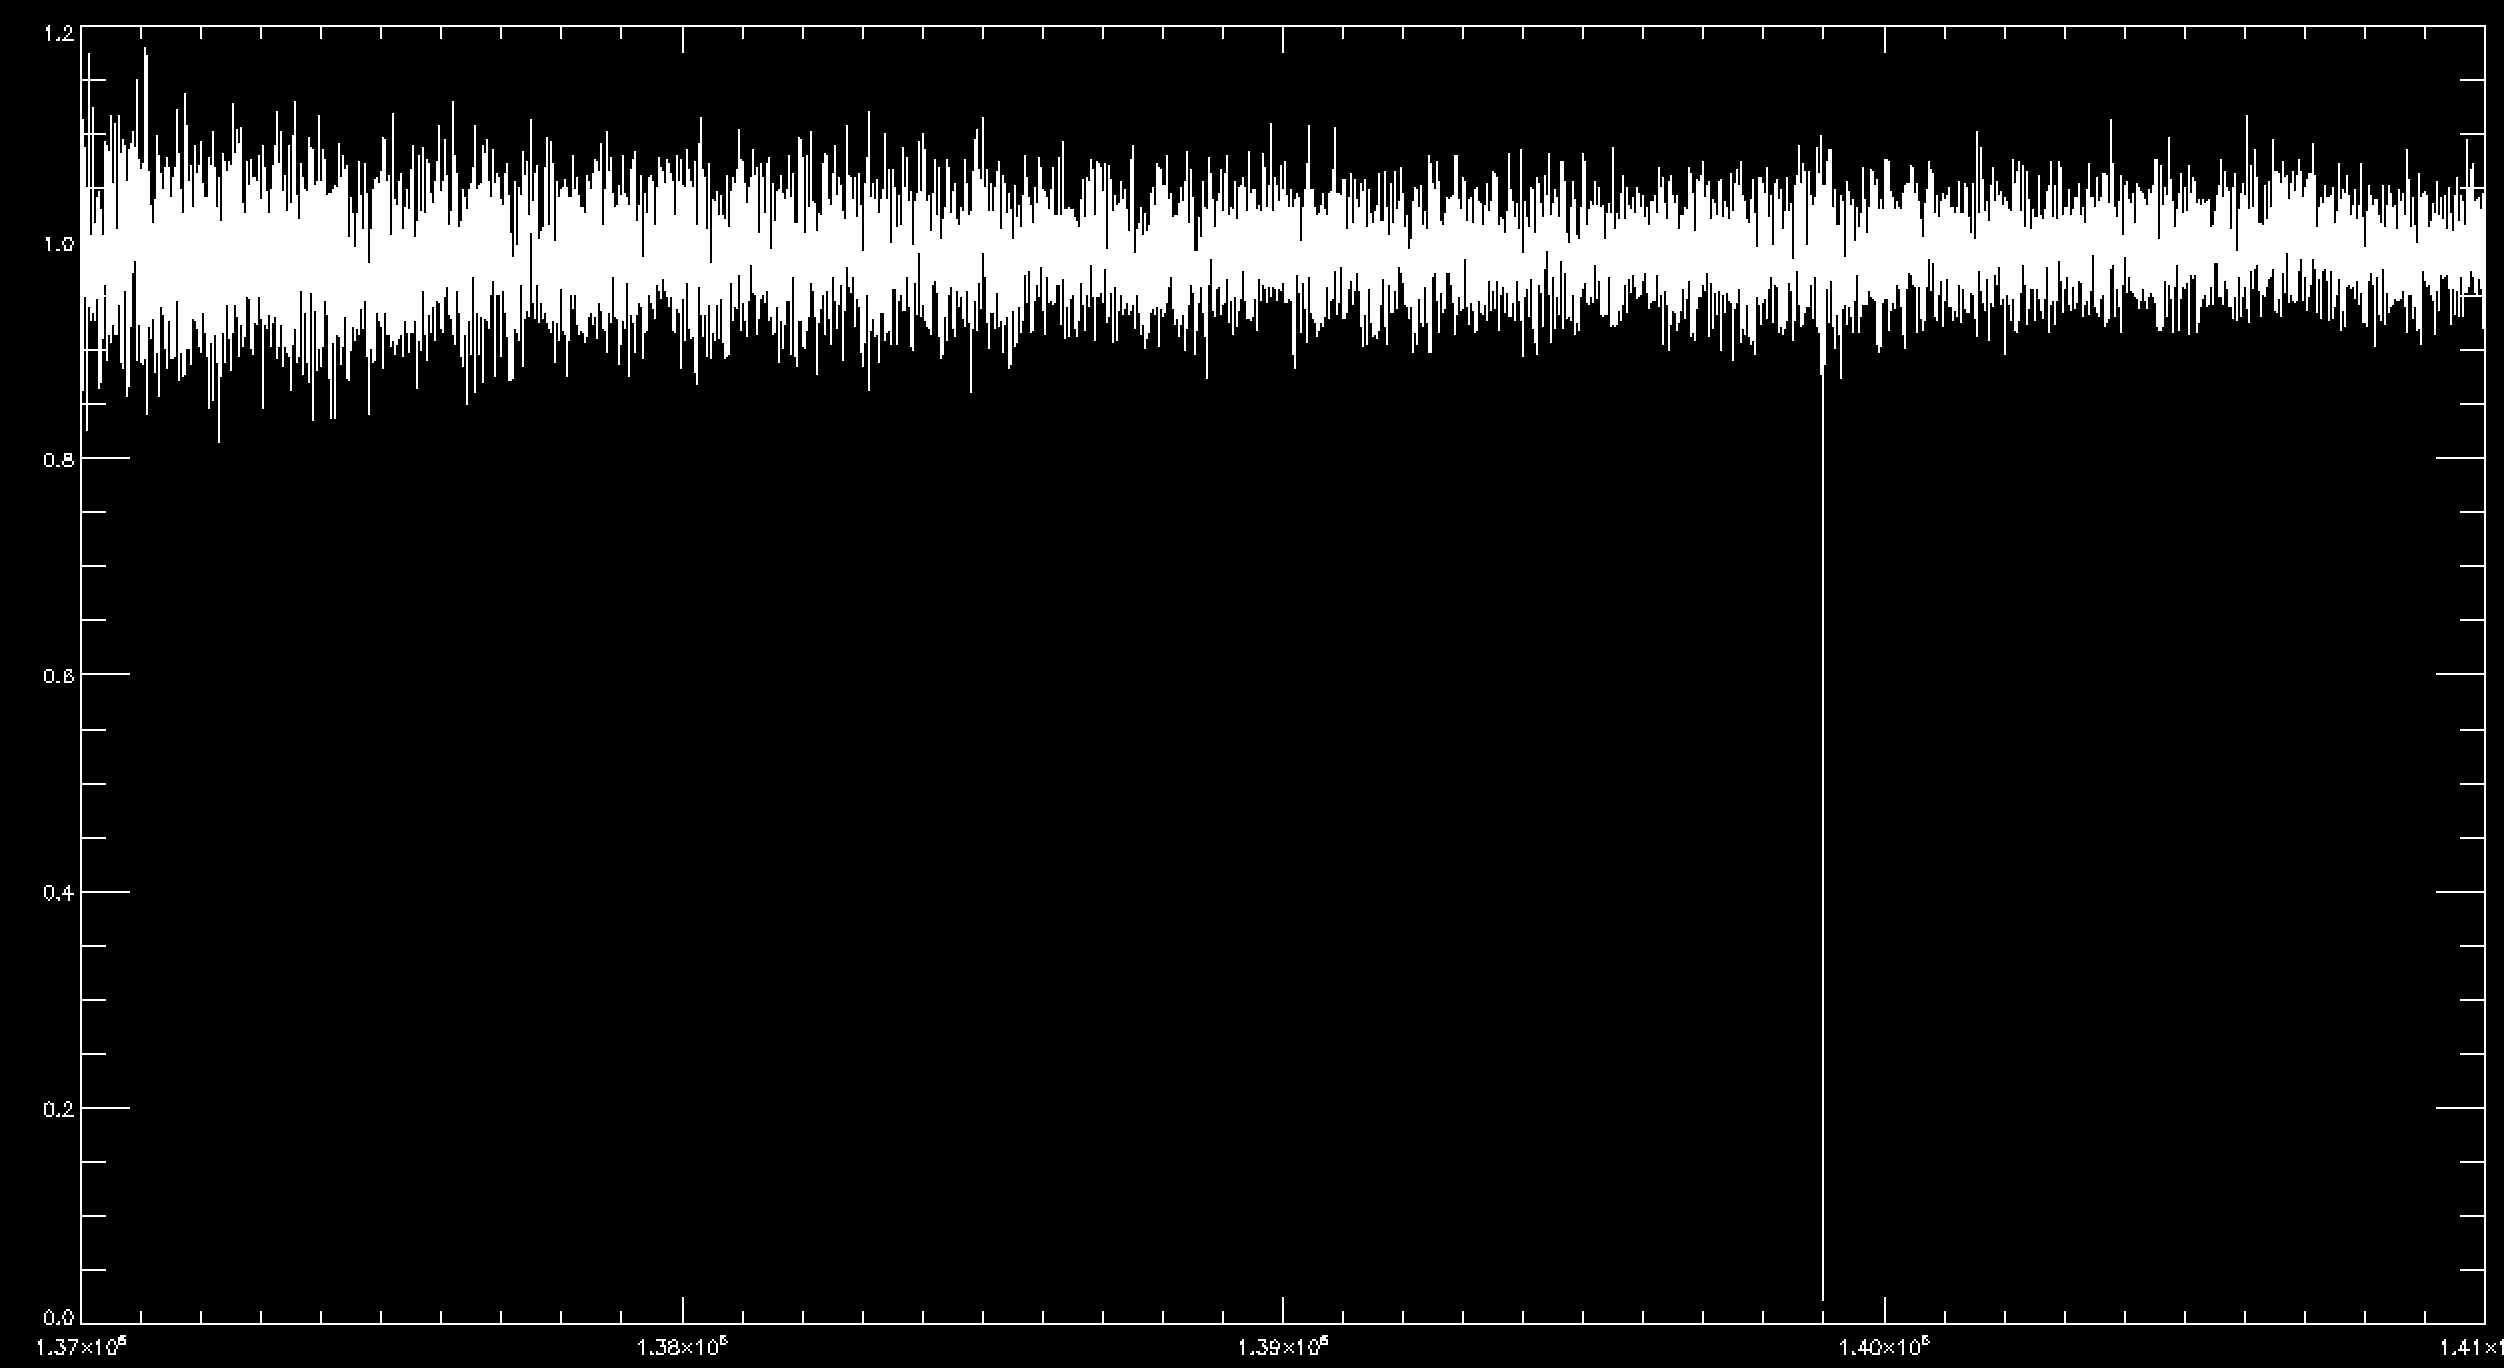
\includegraphics[width=\textwidth]{F-Ring}
    \end{subfigure}
    \begin{subfigure}[b]{0.49\textwidth}
        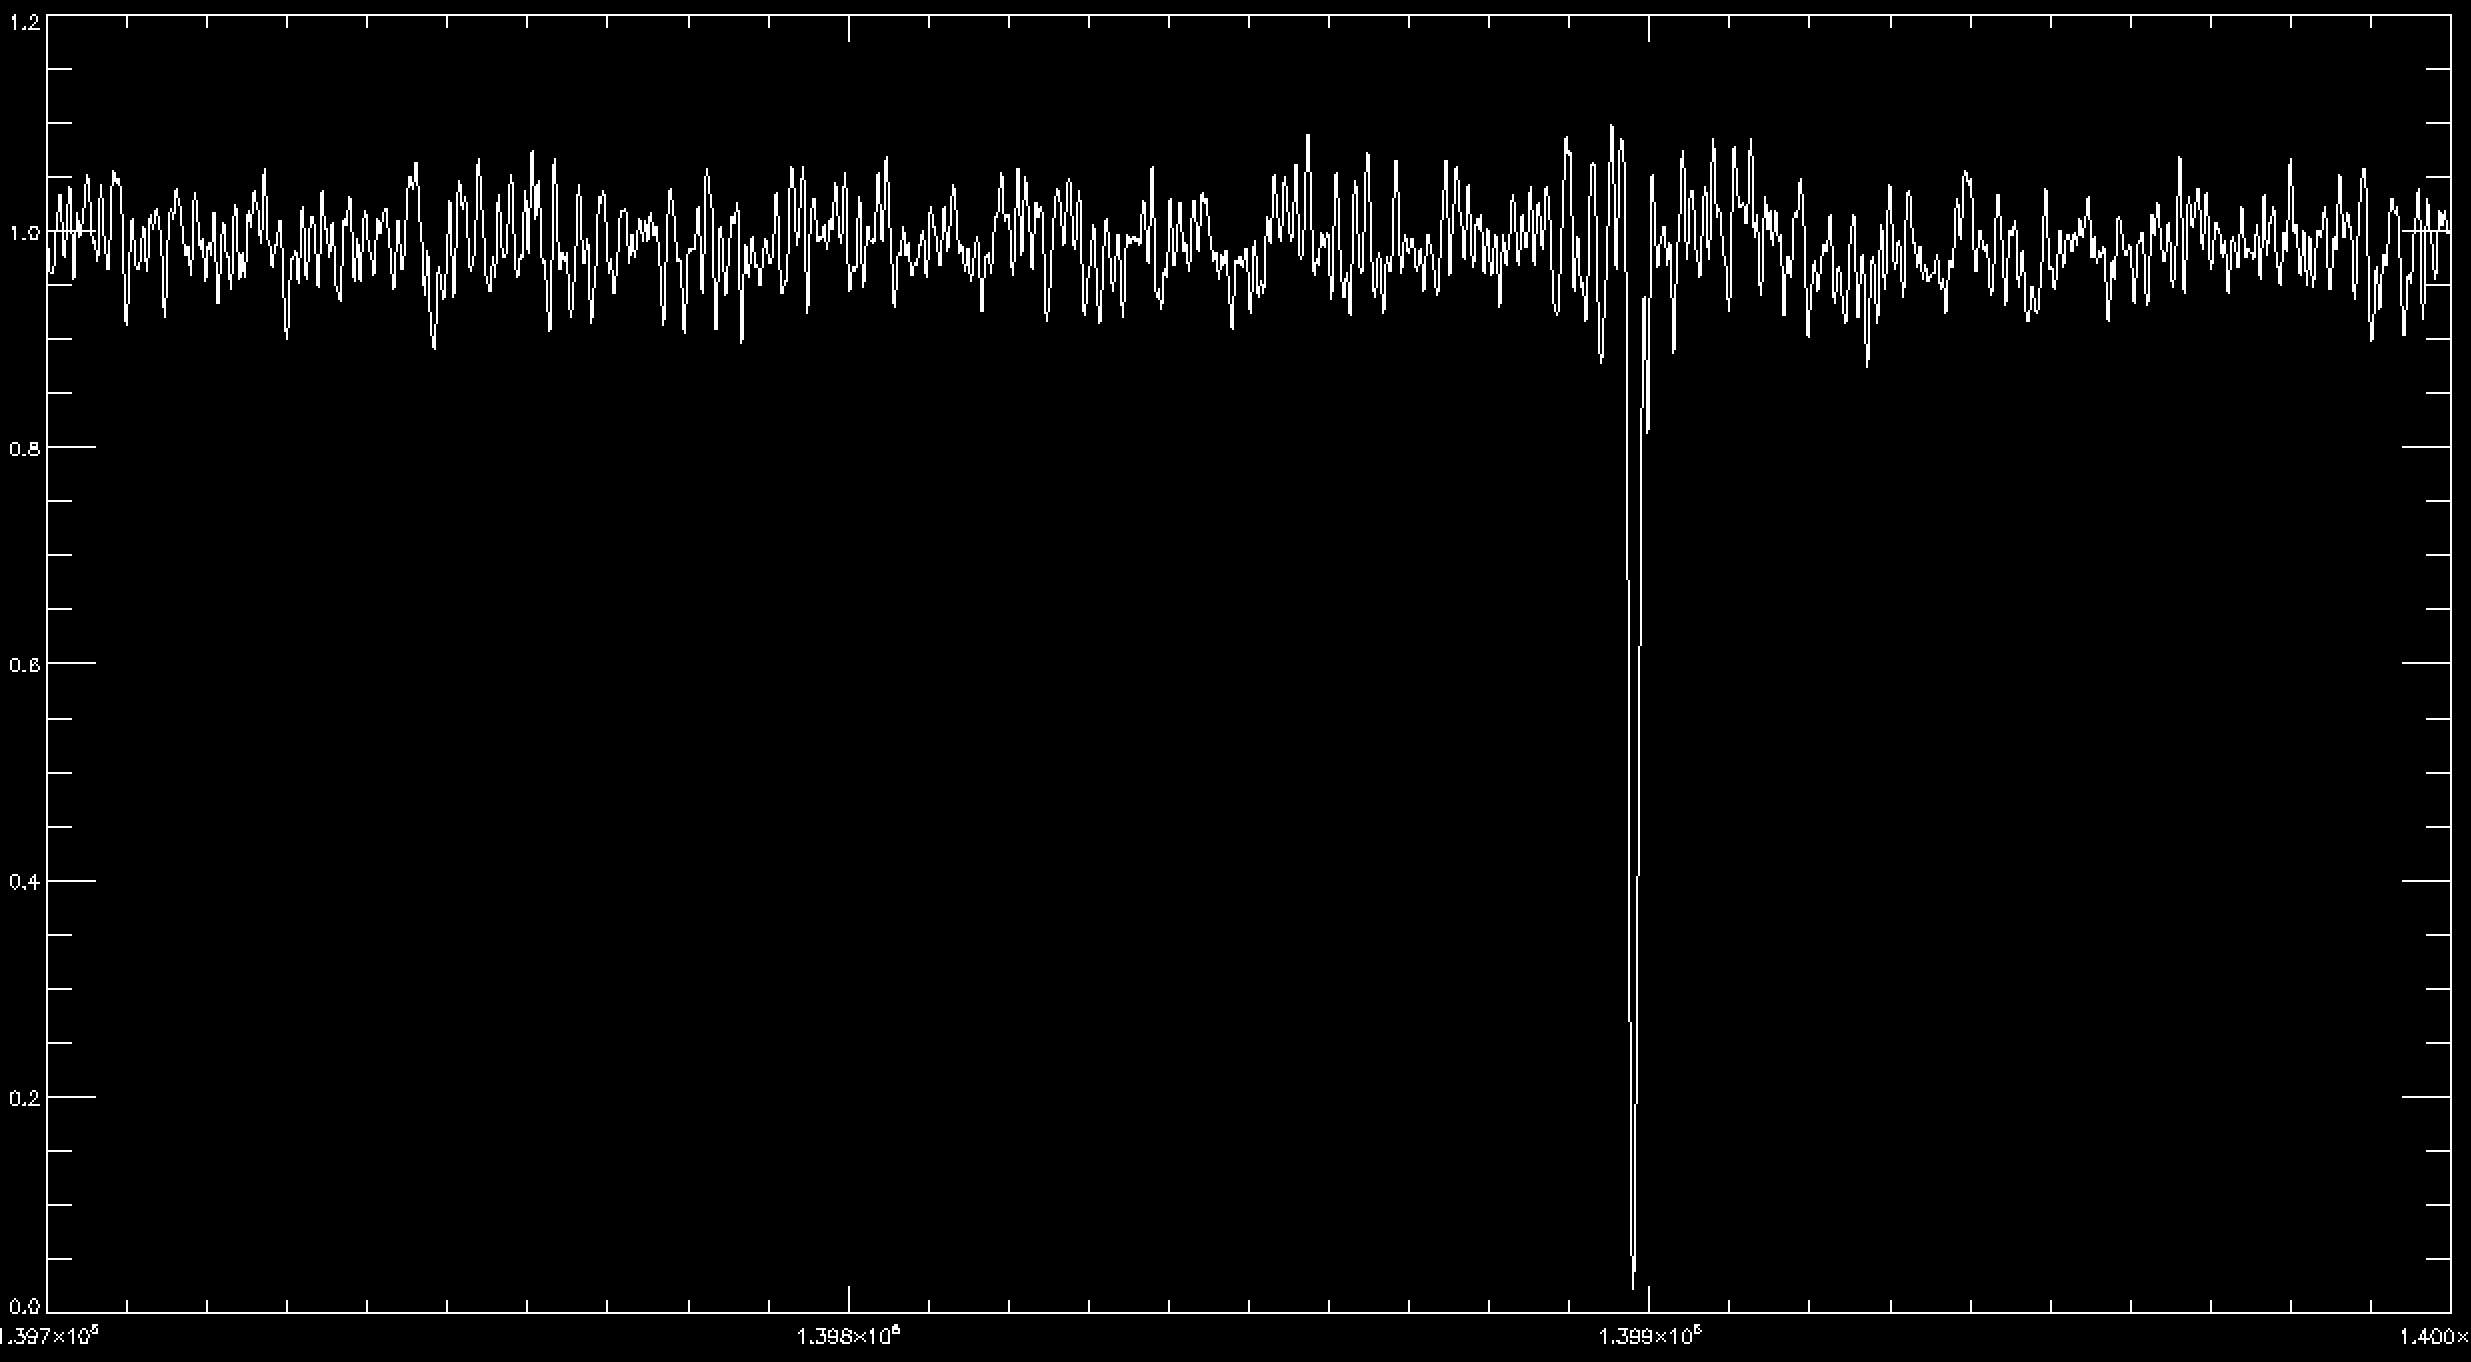
\includegraphics[width=\textwidth]{F-Ring_Zoomed_In}
    \end{subfigure}
\end{figure}
Ryan - Blue means done. Red means description.
\begin{itemize}
    \item \textcolor{blue}{Create your version of Figs 6 and 8 to be included in the interim report (send primitive version of plot program to Dick, who can reformat this to mimic Essam’s style and add it to the interim report) - rjm\_diff\_corr\_compare.pro}
    \item \textcolor{blue}{Contact Glenn and Jolene about the appropriate input files for you to use for the final Rev007 1 km reconstructions for Jolene to post in our prototype PDS directories, crank out those reconstructions using the best assumed resolution to match Essam's.} - \textcolor{red}{Use Rev007\_E\_X43\_struct\_input\_v2.sav for rev 7.}
    \begin{itemize}
        \item \textcolor{red}{Compare rev007 E phase with Essams - rmaguire/v5/compare/rjm\_diff\_corr\_compare.pro uses Essam’s data, and compares the TC reconstruction to Essam’s reconstruction. V5 has 0.3\% error in power. Phase matches up very well.}
    \end{itemize}
    \item \textcolor{blue}{Do the same for the Rev 133, and send files to Glenn so that he can produce diffraction-corrected profiles for Fig. 12 of the interim report.}
    \begin{itemize}
        \item \textcolor{blue}{Make reconstruction fro rev-123 S, X, Ka for F-ring. Replace Dick’s figures in interim report. - Half done. Have not added figures to report.}
        \item \textcolor{blue}{Use Essam’s data for rev-133 and compare reconstructions.}
        \begin{itemize}
            \item \textcolor{red}{Error in doing so for rev-133 with v5. The Riemann sum method for the massive windows that rev-133 has is insufficient in capturing the details of the rapidly oscillating exp(ipsi). Use v4.1 or v4 for rev-133 and rev-123.}
        \end{itemize}
    \end{itemize}
    \item \textcolor{blue}{I don't think Essam detected the F ring on Rev 133, but take a look anyway at your reconstruction in the expected vicinity of the F ring ($\pm$ about 300 km of 140219 km)}
    \begin{itemize}
        \item \textcolor{blue}{F-Ring is 1km in width, roughly. Use appropriate resolutions. - S-Band at 500m resolution detected it.}
    \end{itemize}
    \item \textcolor{blue}{Try your idea of improving your 10 km resolution model for the Titan ringlet, to compare with the User's Guide version. Use 250m resolution for this.} - \textcolor{red}{If I cheat and multiply by about 5, and smooth a wee bit, it looks great...}
    \item \textcolor{blue}{Have you succeeded in doing a direct integration, without FFTs, for the inversion process? This would be good to have working, and to know the time it takes.} - \textcolor{red}{v5 is done. For rev007 E it matches better to Essam’s reconstruction than v4.1, and also is computed in a shorter amount of time. For rev-133 the integral is insufficient. Need to look into better numerical integration techniques.}
    \item You'd worked on a 'forward' code that would produce a synthetic diffraction pattern for a given occultation geometry and assumed radial profile of normal optical depth. This would be a great addition to our software package and would provide a nice test of our inversion code, to be able to retrieve the input optical depth profile by inverting the synthetic diffraction pattern.
    \item Start thinking about the organization of our pipeline processing - a flow chart, if not actual program and procedure names - and especially about how and where users could enter the process mid-stream to perform diffraction corrections to snippets of data at requested resolutions without having to go through the entire preprocessing procedure for an entire RSR file. - Ryan will use LaTex to format what we wrote on the board
\end{itemize}
\subsubsection{\footnotesize RE: Good Plots}
IDL\_pipeline\_v2/gjs\_progress\_report/rjm\_fig\_3-12/gjs\_rev7E\_X43\_huygens\_1km.pro\\
For legends, you can make actual legends using the plot function. However, the plot function’s pretty janky so nobody uses it. In the plot procedure (which all the cool cats use), you can just add text to the plot using “xyouts”. For making arrows, there’s an arrow procedure in IDL where you can just specify the start and end points of the arrow. I have a weird problem where I don’t actually have a procedure named arrow, but instead I have one named “arrow\_internal”. If you end up having the same problem where you only have this “arrow\_internal” thing, then you can still use all the same syntax and everything that’s online for the arrow procedure - you just have to say “arrow\_internal” for every time they say “arrow”.
\subsubsection{\footnotesize RE: A Though on Phase}
While looking through the v5 code, I noticed something. A while back I made psi positive, just because it matched Marouf, and then filed this under `Deal with later.' Psi is a purely geometrical factor. The integral is:
\begin{equation*}
    \int|\hat{T}|w(\rho-\rho_{0})e^{i(\theta-\psi)}d\rho
\end{equation*}
What is written is:
\begin{equation*}
    \int|\hat{T}|w(\rho-\rho_{0})e^{i(\theta+\psi)}d\rho
\end{equation*}
Now, if the phase is negative, this `almost' swaps things back to normal (But it doesn’t exactly, which is really weird as to why it worked to begin with. This is actually quite amazing). But what if, rather than the phase being negative, T runs clockwise. That is $\hat{T}=|\hat{T}|e^{-i\theta}$. This would fix the integral equation, and would also explain why, in order to get reconstructed phase to match essam, we need to do $\arctan(\frac{\Re(T)}{\Im(T)}$. Essam never specifies a clockwise or counter-clockwise preference. A way to test this is with a forward code. If the forward diffraction of the reconstructed T has real and imaginary parts swapped, then we'll know his phase runs clockwise. I ran reconstruction with this new mathematical scheme, and got 0.05\% error on Maxwell, using Essam's data. I think I should keep this scheme, perhaps as a v5.1 or something like that, just in case we need to go back to the old one. Comparison can be found here:\\
rmaguire/v5/compare/comparisons/2018\_01\_25\_rev007\_E\_X43\_Essam\_Comparison\_Titan\_Ringlet\_res\_1000m\_v5\_code\_1.sav\\
-Ryan\\
I agree that changing the sign of theta is the same as assuming that the phase in the complex plane rotates clockwise rather than CCW. Eq 15 in the User's Guide looks to me like it is a CCW rotation, though. But is it that case that you get something different from a 0.05\% error on Maxwell when you change the sign and use the opposite sense of rotation? -Dick\\
The two different codes are: v5 $\hat{T}=|\hat{T}|e^{i\theta}$, $ker=we^{i\psi}$, v5.1 $\hat{T}=|\hat{T}|e^{-i\theta}$, $ker=we^{-i\psi}$. They both produce about 0.05\% errors. Also, I don't think a simply rotation would fix the phase. A rotation of pi/2 would give phase = atan(real / -imaginary). A rotation, and then a reflection, would give phase = atan(real/imaginary), which is what we're seeing, and which is what the clockwise phase would do. As to why the code that has a positive i psi in the exponential works, I have no idea. -Ryan
\subsubsection{\footnotesize RE: Cassini Radio Ring Occultations During the Finale}
I have not done this, but I think you would be safe if you simply left out the data some 100s of km outside of the rings. There are diffraction affects that modify the phase of the signal at high spatial frequencies that you presumably average over. If you have a specific orbital pass you'd like me to look into in more detail. I'd also check with Luciano and Paolo to see what they do about ring occultation data. -Dick\\
Dick, We are struggling mightily to get a gravity field for Saturn to use in the final reconstruction. It appears that the rings are affecting the radio signal during the 5 gravity passes and are corrupting the gravity fit. We find that deleting the data during the ring occultations really helps the fit. However, we are basing our occultation deletes on the assumed ring radii and the associated ring occultation model. Do you know if there has been a determination of the actual times that the radio signal was significantly affected by the rings? -Bob\\
HI, All - Here is a request from a JPL colleague - would you take a look at the X band data for the rev with 23 June 2017 periapse? This is one of the ones with strange geometry, where the rings are occulted several times. It will be a good test of our software and we'll be able to tell Bob whether we see strange effects due to the rings. Add this to your list for when you want to do something different. A starting point would be for Jolene to identify the filename and to compute the occultation geometry over the course of the RSS file - plotting R(t) will look strange, I think! I'd still like to keep on schedule to get our interim report working. Ryan, let's start defining phase in a way that will match Essam's and the inversion code -- let Glenn know how to change his codes to do this. This will make our phase plots agree with Essam's without changing anything, and we'll just report that to get a match, we use the definition of phase that corresponds to a clockwise rotation in the complex plane - is that what you concluded, Ryan? -DF
\end{document}